\documentclass[bibnumbers, palatino]{apuntes}

\title{Ecuaciones en Derivadas Parciales}
\author{G. Guridi, E. Miravalls, G. Julián}
\date{15/16 C2}

% Paquetes adicionales
\usepackage{tikztools}
\usepackage{fancysprefs}
\usepackage{enumitem}
\usepackage{fastbuild}
% --------------------

\precompileTikz

\setcounter{tocdepth}{3}

\bibliographystyle{plainnat}

\begin{document}
\pagestyle{plain}

% http://tex.stackexchange.com/a/14243
%\relpenalty=10000
%\binoppenalty=10000

\begin{abstract}
Estos son los apuntes del curso de Ecuaciones en Derivadas Parciales (2016), del profesor Jesús García Azorero. Es recomendable también mirar los apuntes del año 2015 \cite{ApuntesEDPRual}, que son del mismo curso aunque con un temario organizado de forma distinta.
\end{abstract}

\maketitle

\tableofcontents
\newpage
% Contenido.

% -*- root: ../EDP2016.tex -*-
\chapter{Introducción}

Antes de empezar con la teoría directamente, vamos a ver primero un ejemplo importante. Es una idea muy simple: queremos saber cómo se propaga el calor. Este problema es uno de los tradicionales de ecuaciones en derivadas parciales, y de hecho motivó varios métodos y toda una teoría (la Teoría de Fourier) con montones de aplicaciones. Aquí simplemente haremos un ejemplo moviendo mucho las manos para ver a dónde nos va a llevar el estudio de estos problemas.

\begin{figure}[hbtp]
\centering
\inputtikz{TransmisionCalor}
\caption{Esquema de la varilla (en negro) aislada y conectada a dos bloques de hielo (temperatura 0)}.
\label{fig:TransmisionCalor}
\end{figure}

Consideraremos una varilla de longitud $L$ aislada, y conectada con dos bloques de hielo. Llamaremos $u(x,t)$ a la temperatura en el punto $x$ en el instante $t$. Sabemos que en $t = 0$ tenemos una distribución inicial de temperatura, y en $t \to ∞$ tenemos que la temperatura será cero (no llega a fundir completamente los bloques de hielo).

Como notación, escribiremos las derivadas parciales con subíndices: $u_t \equiv \pd{u}{t}$, $u_{xx} = \pd[2]{u}{x}$, y similar.

Para estudiar el problema, vamos a ver que ocurre en el intervalo $[x, x+h]$. La temperatura, al final nos da una medida de la energía de los puntos. Si la sumamos en ese intervalo obtendremos una cantidad de calor acumulada en ese intervalo. Es decir, $\int_x^{x+h} u(s,t) \dif s$ es la cantidad de calor en el instante $t$ en $[x,x+h]$. Lo interesante es que esa cantidad de calor varía a lo largo del tiempo. Como la varilla está rodeada de aislante, la cantidad de calor sólo se puede estar perdiendo a través de los extremos.

Suponemos que podemos meter la derivada dentro de la integral (habría que demostrarlo), así que podemos decir que \(  \od{}{t} \int_x^{x+h} u(s,t) \dif s = \int_x^{x+h} u_t(s,t) \dif s \label{eq:intro_1}\)

La difusión de la temperatura será, según la ley de Newton, proporcional a la temperatura en el punto que estemos considerando\footnote{Como no somos físicos, la constante es 1.}. Si en el extremo derecho tenemos una derivada positiva (con respecto a x), estamos aportando calor al intervalo. Si tenemos derivada positiva en el extremo izquierdo, estamos perdiendo calor en el intervalo.

Tenemos entonces que ese intercambio de calor es proporcional a \[u_x(x+h, t) - u_x(x,t)\]

Por la regla de Barrow\footnote{Corolario del Teorema Fundamental del Cálculo} podemos decir que \[ u_x(x+h, t) - u_x(x,t) = \int_x^{x+h} u_{xx}(s,t) \dif s\]
Con esto, hemos desarrollado el lado derecho de la ecuación \ref{eq:intro_1}, y pasando el lado derecho restando, combinando las integrales\footnote{Los límites de integración son los mismos así que lo podemos hacer.}, y multiplicando por $\frac{1}{h}$ (ahora veremos por qué) tenemos que
\( \frac{1}{h} \int_{x}^{x+h} u_t(s,t) - u_{xx}(s,t) \dif s = 0 \label{eq:intro_2}\)

Si definimos $$F(x) = \int_{0}^{x} u_t(s,t) - u_{xx}(s,t) \dif s $$ entonces \ref{eq:intro_2}, por definición de cociente incremental, es:
\( \ref{eq:intro_2} = \frac{F(x+h) - F(x)}{h} = 0  \label{eq:intro_3}\),
y aplicando el límite $h \to 0$ y por el Teorema Fundamental del Cálculo, obtenemos que \ref{eq:intro_3} tiende a
\[ F'(x) = u_t(s,t) - u_{xx}(s,t) \]

Luego como \ref{eq:intro_3} era igual a 0, tenemos que,
\[ u_t(x,t) - u_{xx} (x,t) = 0, \forall x \in (0,1), \forall t > 0\]

El problema que tendremos que resolver es entonces que
\[ u(0,t) = u(L,t) = 0 \quad \text{ para } t > 0 \]

¿Cómo resolver esto? Buscaremos que $u(x,t) = X(x) · T(t)$, es decir, que podamos {\bf separar las variables}. En ese caso, tenemos que la ecuación pasa a ser \[ u_t - u_{xx} = 0 \implies XT' - X''T = 0 \implies \frac{X''}{X} = \frac{T'}{T} \]\index{Método!separación de variables}

La igualdad se debe cumplir $∀x ∈ (0,L)$ y $∀t > 0$. Tenemos a dos ecuaciones que dependen de dos variables distintas y que son iguales, luego debe existir un $λ ∈ ℝ$ tal que $\frac{X''}{X} = \frac{T'}{T} = λ$, y nos movemos al mundo de las ecuaciones ordinarias, llegando al sistema  \[ \begin{cases*} T' - λT = 0 \\ X'' - λX = 0 \end{cases*}\]

El problema es que no sabemos qué es λ, así que tenemos que irnos al resto de condiciones del problema. Sabíamos que en los extremos la temperatura es 0, así que tenemos que añadir esas condiciones $X(0) = 0 = X(L)$.

Sin embargo, lo que estudiábamos en EDO\citep{ApuntesEDO} era el problema de Cauchy, en el que teníamos valores sobre la función y su derivada en el mismo punto. Este es un problema de contorno, que se queda fuera del temario de EDO. Como tenemos una solución trivial ($X = 0$), tendremos que buscar para qué valores de λ no se cumple el teorema de existencia y unicidad.

Lo que sí sabemos resolver es ver qué tipo de soluciones tenemos para ${X'' - λX = 0}$. Para ello, resolvemos el polinomio característico. Para $λ = 0$, tenemos que $X(x) {= a+bx}$. Como $X(0) = 0 = a$, y $X(L) = bL = 0$, tenemos que $X \equiv 0$, y no nos vale porque es una solución trivial.

Buscamos ahora ver qué pasa con $λ > 0$. Podemos decir perfectamente que $λ = μ^2$. En este caso, tendríamos que las soluciones son $X(x) = ae^{μx} + be^{-μx}$. Sin embargo, las condiciones de contorno nos dirán que $a = b = 0$, lo que nos lleva a otra solución trivial.

Nos falta probar qué pasa con $λ < 0$. Igual que antes, ponemos $λ = -μ^2$. Repasando de nuevo el curso de EDO, tenemos que $X(x) = a \cos μx + b \sin μx$. Con las condiciones de contorno tenemos que $X(x) = b \sin μx$ y con la constante $μ = \frac{kπ}{L}$ para $k = 1,2,3,\dotsc$.

Las soluciones serán entonces de la forma \[ X_k = b_k \sin \left(\frac{kπ}{L} x\right)\] correspondientes a los autovalores $λ_k = -\left(\frac{kπ}{L}\right)^2$. % \lambda < 0

Por otra parte, miramos qué ocurre con $T$ para $\lambda < 0$: resolviendo tenemos que $T_k(t) = c_k e^{λ_k t}$, así que las soluciones particulares de la ecuación del calor son \[ u_k(x,t) = a_k e^{-\left(\frac{kπ}{L}\right)^2t} \sin \left(\frac{kπ}{L} x \right) \]

Pero no hemos terminado el problema: nos falta meter el dato inicial $u(x,0) = f(x)$. Por ejemplo, si $f(x) = 5 \sin \left(\frac{2π}{L} x\right)$ entonces $u(x,t) = 5 e^{-\left(\frac{2π}{L}\right)^2t} \sin \left(\frac{2π}{L} x\right)$.

Como la ecuación es lineal, también podemos sacar la solución para funciones que sean sumas de senos; y utilizando la propiedad de que dadas dos soluciones particulares, si las sumamos también es solución, podemos llegar a la idea de Fourier.

¿Nos vale con sumas de senos? La respuesta es que sí: Fourier dice que cualquier función se puede escribir como suma infinita de senos, y por lo tanto siempre podemos encontrar la solución: \[ f(x) = \sum_{k=1}^∞ a_k \sin \frac{kπ}{L} x\]

\newpage % FIXME: puede crear una página en blanco en medio del documento
La cuestión es que ahí nos encontramos con toda una serie de problemas:
\begin{itemize}[itemsep = 1pt]
	\item La serie es alternada y no sabemos si converge.
	\item No sabemos cómo se calculan los $a_k$.
	\item No sabemos exactamente qué significa que una función sea igual a una serie infinita.
	\item No sabemos si la derivada de la función es igual a la derivada de la serie.
\end{itemize}

Todos estos problemas son los que motivan el análisis funcional\citep{ApuntesAnalisisFuncional} y las matemáticas del siglo XIX. Nosotros los veremos en este curso en el \fref{chap:EcuacionesSegundoOrden}.


% -*- root: ../EDP2016.tex -*-
\chapter{Ecuaciones de primer orden}

\section{Modelo de un atasco}

	Vamos a empezar con un modelo sencillo. Observemos el fenómeno del embotellamiento fantasma, el cual tiene una ecuación bastante sencilla. Veamos como se generan esos atascos y como se disipan.

	Estudiaremos una función que nos de la densidad de coches en un punto, en el tiempo.

	$$u(x,t) = \text{densidad}$$

	Observemos un modelo muy simple en el que solo hay un carril y los coches fluyen solo en una dirección.

	(DIBUO DE LA RECTA CON FLECHA HACIA LA DERECHA)

	La variación en el número de coches de un intervalo será:
	\[ \od{}{t} \int^{x+h}_{x} u(s,t) \dif s = \int^{x+h}_{x} u_t(s,t) \dif s \]

	Esto equivale a al número de coches que entran por $x$ menos los que salen por $x + h$. Es decir, tenemos un flujo $q(u, x, t)$. Si suponemos que nos fijamos en un instante lo suficientemente pequeño en un tramo pequeño podemos asumir que depende solo de $u$. En ese caso, si $q > 0$ el flujo sería hacia la derecha.
	\[ q(u(x,t)) - q(u(x+h,t)) = -( q(u(x+h,t)) -  q(u(x,t)) ) \eqexpl{Barrow} -\int^{x+h}_{x} [q(u)]_{x}
	\]

	Por lo tanto, tendremos sistemas del tipo:
	\begin{equation*}
	\left\{
	\begin{array}{rl}
	u_t + [q(u)]_{x} =&\! 0 \\
	u(x, 0) =&\! F(x) \quad \quad \text{dato}
	\end{array}
	\right.
	\end{equation*}

	Ahora debemos probar distintas funciones $q$ y tratar de resolver el sistema.

	\subsection{Modelo básico}

		Tomando $q(u) = cu$.

		\begin{equation*}
		\left\{
		\begin{array}{l}
		u_t + cu_x = 0 \\
		u(x,0) = F(x)
		\end{array}
		\right.
		\end{equation*}


		Esta ecuación dice que el flujo es proporcional a la densidad. Implica que los coches se mueven con velocidad constante, a más velocidad más flujo y viceversa. Si en el instante inicial tenemos una función de la densidad respecto de las zonas del tramo, según pasa el tiempo la densidad se irá desplazando hacia la derecha manteniendo la misma forma.

		(DIBUJO)

		\textbf{Comprobación:}

		$$ u(x,t) = F(x-ct) $$
		$$ u_x(x,t) = F'(x-ct)$$
		$$u_t(x,t) = F'(x-ct)*(-c)$$

		$$ \{ u_t + cu_x = … = 0 \quad\quad u(x,0) = F(x) \} $$

		\subsubsection{Representación gráfica}


			$$u(x,t) = \text{Cte.}$$
			$$F(x - ct) = \text{Cte.}$$

			Conclusión: $x-ct = k$.


			Las soluciones dependiendo de k se desplazan por el plano siguiendo una recta de inclinación $c$. Siguiendo una fórmula del tipo $x-ct = k$. Con esto se puede obtener como avanzan los datos (densidades) respecto de un instante inicial.

			Esto son los conjuntos de nivel de las soluciones.

			(DIBUJO)



	\subsection{Otro ejemplo}

		Imaginemos un río con una velocidad constante, en el que a partir de un punto realizamos un vertido. El río tiene velocidad $v$ y en $x=0$ realizaremos una contaminación $\beta(t)$. En $t=0$ consideraremos que está limpio.

		Tenemos las ecuaciones:

		$$u_t + vu_x = 0$$
		$$u(x,0) = 0 \quad (x>0) $$
		$$u(0,t) = \beta(t), t>0$$


		Resolvemos el problema igual que antes, buscamos los conjuntos de nivel que serán rectas como nos ha salido antes. Vamos a buscar esas rectas.

		\textbf{Buscamos $x(t)$ tal que $u(x(t),t)$ sea constante}

		Derivando en t: $u_x x' + u_t = 0$ que junto con la ecuación $u_t + v u_x = 0$ nos da que $x' = v \Rightarrow x = x_0 + vt $.

		Las características saldrían \(x-vt = \text{Cte}(=x_0) \label{eq:rio_vcte}\).

		Esas son nuestras rectas conjuntos de nivel, que en este caso indicarían el frente de la contaminación, el límite a partir del cual el río sigue limpio.

		$$u(x,t) =
			\begin{cases}
				0                      & (x-vt) > 0 \\
				\beta(t - \frac{x}{v}) & (x-vt) < 0
			\end{cases}
		$$

		\begin{figure}[hbtp]
			\centering
			\inputtikz{ContaminacionRio}
			\caption{}.
			\label{fig:ContaminacionRio}
		\end{figure}

		El valor de $u(x,t)$ cuando $x-vt < 0$, se obtiene utilizando \ref{eq:rio_vcte} y tomando el punto de corte de la recta $x-c \cdot t=k$ que pasa por $(0,t^*)$:

		$$
		\begin{rcases}
			0 - vt^{*} = k \\
			x - vt = k
		\end{rcases}
		 \Rightarrow x-vt = -vt^{*} \iff t^* = \frac{x-vt}{-v} = t - \frac{x}{v}$$

		Por lo que
		$$u(x,t) = \beta(t^*) = \beta(t - \frac{x}{v}), \quad \text{ cuando } x - vt < 0$$

		De esto obtenemos una función de x en función del tiempo que nos permite saber cuándo una parte del río se contamina.

	\subsection{Ejemplo más avanzado}

		Supongamos que existe descomposición biológica:

		$$u_t + vu_x = -\gamma u$$
		$$u(x,0) = \text{Cte}$$
		$$u(0,t) = \beta$$

		(Cambiamos de variable)

		$$u_t + \gamma_u + vu_x = 0$$
		$$e^{\gamma t} u_t + e^{\gamma t} u + v e^{ \gamma t} u_x = 0 $$

		lo que es lo mismo

		$$(e^{\gamma t}u)_t + v (e^{\gamma t} u)_x$$

		Y definimos la función $W$:

		$$W = e^{\gamma t}u$$.


		Hay que comprobar cuál es el efecto del término de descomposición biológica ($-\gamma u$). ¿ $W(x,0)$ , $ W(0,t)$ ?. Esto queda como ejercicio al lector.


	\subsection{Modelo con aportación externa}

		$$u_t + vu_x = f(x,t)$$
		$$u(x,0) = F(x)$$

		Ya al no ver constante, la solución no va a ser constante a lo largo de las características, que siguen existiendo. En el caso $f = 0$ éstas daban la solución, pero ahora van a influir.


		\subsubsection{Solución 1}

			Cambio de variables:
			$$z = x-vt$$

			Lo cual hace más sencillo observar la variación temporal. Continuamos el cambio:
			$$x = z + vt$$
			$$W(z,t) = u(z+vt, t)$$

			Entonces queremos estudiar la variación de $W$ respecto del tiempo:

			$$W_t(z,t) = u_x(z + vt, t)v + u_t(z+vt, t) = f(z + vt, t)$$

			Integramos:
			$$W(z,t) = W(0,t) + \int^{t}_{0} f(z+v\tau, \tau) d\tau $$

			Lo que se entiende como el dato inicial más la suma de las aportaciones de esta función $f$ en el tiempo pasado. Ahora deshacemos el cambio de variable:

			$$u(z + vt, t) = u(z,0) + \int^{t}_{0} f(z+v\tau, \tau) d\tau$$
			$$z = x-vt$$
			$$u(x,t) = u(x-vt,0)+ \int^{t}_{0} f(x-v(t-\tau),\tau) d\tau$$

			(donde $u(x-vt,0) = F(x-vt)$)

			Esto es un milagro ya que tiene una fórmula explícita, que es poco común en EDOs y EDPs.

		\subsubsection{Solución 2}

			Vamos a descomponer el sistema en 2. Dos soluciones en las que cada una va a ser solución de dos partes del problema que nos interesan. Una del dato inicial y otra del resto.
			$$u = \phi + \psi$$

			Por un lado:
			$$
			\begin{rcases}
				\phi_t + v\phi_x = 0 \\
				\phi(x,0) = F(x)
			\end{rcases}
			\rightarrow \phi(x,t) = F(x-vt)
			$$

			Y por otro:
			$$\psi_t + v\psi_x = f(x,t)$$
			$$\psi(x,0) = 0$$

			Este problema con \concept{DUHAMEL} (la fuente externa se interpreta como una fuente de datos iniciales, se cambia el cero de la segunda ecuación de las anteriores) se puede interpretar como que tenemos una función que transporta el sistema.

			\begin{figure}[hbtp]
				\centering
				\inputtikz{interseccionCaracteristica}
				\caption{}
				\label{fig:interseccionCaracteristica}
			\end{figure}



			$$\xi_t + v\xi_x = 0$$
			$$\xi(x,s) = f(x,s)$$

			Continuamos:
			\(\xi(x,t) = f(x^*,s) \label{eq:modelo_aportacion_externa_1}\)
			$$
			\begin{rcases}
				x-vt = k \\
				x^* - vs = k
			\end{rcases}
			 \rightarrow x-vt = x^* - vs
			$$
			\( x-v(t-s) = x^{*} \label{eq:modelo_aportacion_externa_2} \)

			Y sustituimos \ref{eq:modelo_aportacion_externa_2} en \ref{eq:modelo_aportacion_externa_1}
			$$\xi(x,t) = f(x - v(t-s), s)$$


			Tenemos la solución correspondiente de un aporte instantáneo en el punto $t$. Por lo tanto la solución será la suma de todos los aportes instantáneos:

			$$\Rightarrow \psi(x,t) = \int^{t}_{0} f(x-v(t-s),s) \dif s $$

			Aunque hemos hecho un montón de asunciones que tendremos que comprobar en algún momento.

	\subsection{Modelo de tráfico más realista}

		No hemos tenido en cuenta que la velocidad de los coches no es totalmente proporcional a la densidad. Si ésta baja mucho, los coches llegan a pararse. Hay una densidad máxima donde el tráfico quedará totalmente estancado (los coches pegados).

		\begin{figure}[hbtp]
			\centering
			\inputtikz{parabola}
			\caption{}
			\label{fig:parabola}
		\end{figure}

		Una función más realista sería una parábola. Si no hay coches no pasa ninguno, pero a partir de un punto cuantos más coches, menos rápido van, y menos pasan.

		$$ q(u) = Au (B-u) = ABu - Au^{2} $$

		Veamos su ecuación:
		$$u_t + [q(u)]_x = 0$$
		$$ … $$
		$$ u_t + (AB - 2Au) u_x = 0 $$

		La velocidad va a ser dependiente de la densidad.

		Nos saldrán características cuya pendiente dependa del valor en el tiempo inicial. Si divergen no habrá problema, pero si convergen, habrá puntos donde rectas de densidad 2 (por ejemplo) cortarán con rectas de densidad 1. Esto se entiende como coches que van más rápido que se encuentran con coches que van más lentos y se ven obligados a frenar.


		Para simplificar los cálculos de este modelo asumamos que $A = B = 1$. Por lo tanto ahora estudiaremos:

		\begin{equation*}
			\left\{
			\begin{array}{l}
				u_t + (1-2u)u_{x} = 0 \\
				u(x, 0) = F(x) \quad \quad \text{dato}
			\end{array}
			\right.
		\end{equation*}

		Obtengamos las características (curvas de nivel para esa solución). Con la regla de la cadena tenemos:

		$$u_x x' + u_t = 0 \text{ a lo largo de la característica}$$

		$$x' = 1 - 2u \eqexpl{$u=k$} 1 - 2k$$

		$$x = x_0 + (1-2k)t$$

		Características:
		\( x - (1-2k)t = x_0\quad,\quad k=F(x_0)  \label{eq:caracteristicas_realistas} \)

		Me fijo en un punto en el instante inicial. Con el valor de ese punto calculamos la pendiente. A lo largo de las caracterísitcas el valor del dato se mantiene. En este caso las caracteristicas no son paralelas porque la pendiente es $1-2k$, es decir, depende de $k$.

		\begin{figure}[!htb]
			\centering
			\inputtikz{rectasDivergentes}
			\caption{}
			\label{fig:rectasDivergentes}
		\end{figure}

		\newpage

		Veamos algunos ejemplos:

		\begin{example}[Semáforo]

			$$F(x) =
			\begin{cases}
				1 & x < 0 \\
				0 & x > 0
			\end{cases}
			$$

			\begin{figure}[!htb]
				\centering
				\inputtikz{semaforoCerrado}
				\caption{Semáforo cerrado en $t=0$}
				\label{fig:semaforoCerrado}
			\end{figure}

			Y en $t=0$ el semáforo está cerrado, en $t>0$ abierto.

			En la sección izquierda: $ F = 1 \Rightarrow x - (1 - 2*1)t = x + t = k \Rightarrow x = k -t $, con $k$ constante.

			En la derecha: $F = 0 \Rightarrow x-t = k$.

			\begin{figure}[!htb]
				\centering
				\inputtikz{caracteristicasSemaforo}
				\caption{}
				\label{fig:caracteristicasSemaforo}
			\end{figure}

			Vemos que las características se abren y se separan desde $x=0$ hacia afuera.

			Por lo tanto las características no nos dan información en la región entre las rectas características que parten del $0$, ya que ninguna característica pasa por ese espacio.

			\begin{figure}[!htb]
				\centering
				\inputtikz{semaforoT}
				\caption{Instante $t=T$}
				\label{fig:semaforoT}
			\end{figure}

			Esto pasa porque no está definida la función en el $0$. Si lo estuviera podríamos intentar sacar infinitas características desde el 0 que rellenaran la zona en la que no tenemos información.

		\end{example}

		\begin{example}[Frenazo]

			Imaginemos ahora dos zonas, una con densidad de coches baja y otra con densidad alta (se encuentran con un atasco)

			\begin{figure}[!htb]
				\centering
				\inputtikz{modeloAtasco}
				\caption{}
				\label{fig:modeloAtasco}
			\end{figure}

			$$F(x) =
			\begin{cases}
				1/5 & x < 0 \\
				2/3 & x > 0
			\end{cases}
			$$

			Dibujamos las características con \ref{eq:caracteristicas_realistas}.

			\begin{figure}[!htb]
				\centering
				\inputtikz{ondaChoque}
				\caption{}
				\label{fig:ondaChoque}
			\end{figure}

			Vemos en este dibujo casos en los que cuando recorremos una recta característica con valor $\frac{1}{5}$ nos encontramos con otra de valor $\frac{2}{3}$. Momento en el cual se produce el frenazo.

			Fijando $T$ podemos mirar el valor de cada $x$ trazando su correspondiente característica. Ahí es donde nos encontraremos los puntos en los que las rectas cortan. La sucesión de puntos de corte en función de $t$ es la curva que nos interesa. Se corresponde a la función que dictamina como se van encendiendo las luces rojas de los coches según se van parando al llegar a un atasco.

		\end{example}

		Intentemos resolver ambos en general. Volvemos a la equación:

		$$u_t +m [q(u)]_x = 0$$

		Como tiene derivadas y nos impide trabajar con funciones con discontinuidades intentaremos ver el origen de esta hasta que no haya derivadas y no hayamos hecho hipótesis de regularidad (obtendremos soluciones débiles). Esta ecuación venía de una integral:

		$$\frac{1}{h} \int^{x+h}_{x} u_t + [q(u)]_x = 0$$

		que a su vez venía de:

		$$\frac{d}{dt} \int^{x+h}_{x} u = q(u(x))-q(u(x+h))$$

		$u$ es $C^1$ a trozos con discontinuidad de salto en $x=s(t)$. Así que llegamos al problema:

		\textbf{Hallar $s(t)$}

		\begin{figure}[hbtp]
			\centering
			\inputtikz{discontinuidadAtasco}
			\caption{}
			\label{fig:discontinuidadAtasco}
		\end{figure}

		% A partir de aquí está bastante mal muy probablemente


		En el intervalo $[x_1,x_2]$:

		$$\frac{d}{dt} \left[ \int^{s(t)}_{x_1} u(x,t) dx + \int^{x^2}_{s(t)} u(x,t) dx \right] = q(u(x_1)) - q(u(x_2))$$


		$$ \text{¿ } \frac{d}{dt} \int^{s(t)}_{x_1} u(x,t) \dif x \text{ ?} $$

		Tomemos:

		$$G(z,t) = \int^{s(t)}_{x_1} u(x,z) \dif x $$

		$$G_z = u(z,t) $$

		$$G_t = \int^{z}_{x_1} u_t(x,z) \dif x $$

		$$\int^{s(t)}_{x_1} u(x,t) dx = G(s(t),t)$$

		$$\frac{d}{dt} \int^{s(t)}_{x_1} u(x,t) dx = G_z (s(t),t) s'^{-} G_z(x,t) = [u(s(t),t) ]^- s'(t) + \int^{s(t)}_{x_1} u_t(x,t) dx$$


		\textit{Queda para el lector hacer lo mismo con la otra integral.}


		\textbf{Notación}

		$$[u(s(t),t)]^{-} = \lim_{x \to s(t)^{-}} u(x, t) $$


		Si realizamos lo mismo con la otra integral llegamos a esta \textbf{conclusión}:

		$$([u(s(t),t)]^{-} - [u(s(t),t)]^{+}) s'(t) +  \int^{s(t)}_{x_1} u_t(x,t) dx + \int^{x^2}_{s(t)} u_t(x,t) dx = q(u(x_1,t)) - q(u(x_2,t)) $$

		Ahora llevamos $x_1$ y $x_2$ tender a $s(t)$.

		Hacemos $x_1 \rightarrow s(t)^{-}$,$x_2 \rightarrow s(t)^{+}$.


		\textbf{Resultado:}

		$$(u(s(t),t)^{-} - u(s(t),t)^{+}) s'(t) = q(u(s(t),t)^{-}) - q(u(s(t),t)^{+})$$

		$$s'(t) = \frac{q(u(s(t),t)^{-}) - q(u(s(t),t)^{+})}{u(s(t),t)^{-} - u(s(t),t)^{+}} $$

		Lo cual resulta ser nuestra equación del shock \concept{Rankine - Huginot}.

		La que vimos en la figura: \ref{fig:ondaChoque}.

		Para obtener la curva calculamos:

		Salto en u: $\frac{2}{3} - \frac{1}{5} = \frac{7}{15}$

		Salto en q: $\frac{2}{3} (1-\frac{2}{3}) - \frac{1}{5}(1-\frac{1}{5})$

		$$q(u) = u (1-u) = \frac{2}{9} - \frac{4}{25} = \frac{14}{225} $$


		Entonces:

		$$s'(t) = \frac{\text{Salto q}}{\text{Salto u}} = \frac{\frac{14}{225}}{\frac{7}{15}} = \frac{14.15}{7.225} \equiv \alpha \quad(>0)$$

		$$s(0) = 0 \Rightarrow s(t) = \alpha t $$

		Por lo que la onda de choque sigue $x = s(t) = \alpha t$.

		(DIBUJO RECTA)


		\subsection{Soluciones generalizadas}

			\begin{itemize}

				\item $ u \in C^1 \text{ en } R^{-} \text{ y en } R^{+}. $
				\item $u$ tiene una discontinuidad de salto a lo largo de la curva $x = s(t)$.
				\item La curva satisface la condición de Rankine-Hugoniot: $s' = \frac{\text{Salto q}}{\text{Salto u}}$.

			\end{itemize}

			\begin{figure}[hbtp]
				\centering
				\inputtikz{OndaChoqueRPM}
				\caption{}
				\label{fig:OndaChoqueRPM}
			\end{figure}

			\begin{example}[pendiente de resolución]

				$$u_t + (1-2u)u_x = 0\footnote{Las curvas características exigen que el lado derecho sea 0. Si no, hay que aplicar el principio de Duhamel, el modelo con descomposición, etc...}$$
				$$u(x,0) = F(x)$$

				Las características son las curvas $(x(t),t)$ tales que $u(x(t),t) = k$.

				Las calculamos:

				$u_x x' + u_t = 0 $

				$x' = 1-2u \eqexpl{$u=k$} 1-2k $

				$x = (1-2k)t + x_0$

				$x - (1-2k)t = x_0$

				Siendo $x_0$ el punto de partida y $k$ el valor que se propaga.

				\begin{figure}[hbtp]
					\centering
					\inputtikz{caracteristicasSemaforo}
					\caption{}
					\label{fig:caracteristicasSemaforo2}
				\end{figure}

			\end{example}

			Para calcular la región intermedia usaremos esta \textbf{idea}: Una aproximación y paso al límite. Imaginemos que $F_\epsilon$ es continua y decreciente.

			\begin{figure}[hbtp]
				\centering
				\inputtikz{FEpsilon}
				\caption{}
				\label{fig:FEpsilon}
			\end{figure}

			Entonces en la región intermedia:

			$$u_\epsilon (x,t) = F_\epsilon (x_\epsilon) \equiv k_\epsilon $$

			Característica: $x - (1-2k_\epsilon) t = x_\epsilon$, con $F_\epsilon(x_\epsilon) = k_\epsilon$

			Y ahora queremos hallar $\lim\limits_{\epsilon \rightarrow 0} u_\epsilon(x,t).$

			Por ser $x_\epsilon \in (0,\epsilon)$, $\lim\limits_{\epsilon \rightarrow 0} x_\epsilon = 0$.

			$$ \frac{x - x_\epsilon}{t} = 1-2k_\epsilon$$
			$$k_\epsilon = \frac{1}{2} (1 - \frac{x-x_\epsilon}{t}) \convs[][\epsilon][0] \frac{1}{2} (1 - \frac{x}{t})$$

			Con lo que llegamos a una fórmula para la densidad en la región intermedia:

			$$u(x,t) = \frac{1}{2} (1 - \frac{x}{t}) \quad \text{ si } (x,t) \text{ está en la región intermedia. }$$

			\begin{figure}[hbtp]
				\centering
				\inputtikz{SolucionTFijo}
				\caption{}
				\label{fig:SolucionTFijo}
			\end{figure}

			$$u(x,T) =
			\begin{cases}
				1 & x \leq -T \\
				\frac{1}{2} (1 - \frac{x}{T}) & -T < x < T \\
				0 & x \geq T
			\end{cases}
			$$

			A esto se le llama la \concept{Onda de rarefacción}. Este resultado no depende de la aproximación que tomemos de $F_\epsilon$, solo que sea continua ya que con el paso al límite la función desaparece.



	\subsection{Cambio de variables. Ecuación de Burgers}

		Dados:

		$$ u_t + [q(u)]_x = 0 \quad (q \in C^2) $$

		$$u_t + V(u)u_x = 0 $$

		Realizamos un cambio de variables:

		$$W = V(u)$$
		$$W_t = V'(u) \cdot u_t$$
		$$W_x = V'(u) \cdot u_x$$

		Y vamos a ver que función cumple $W$. Lo que hacemos es pasar a escribir la ecuación en terminos de una variable que es la "velocidad" (CUIDADO CON LA INTUICIÓN), al contrario que antes, que era de la densidad. Esta velocidad es la velocidad de $u$, la velocidad a la que se propaga la densidad. No tenemos que entenderla como la velocidad de los coches.

		Imaginemos un mapa de tráfico en el que se ve la densidad del tráfico con colores. La $W$ es la velocidad a las que esas manchas de color se desplazan, no los coches en sí. Están relacionadas pero no son lo mismo.

		Completemos el sistema anterior con $W$:

		\(u_t + V(u) u_x = 0\quad\quad (u \equiv \text{densidad}) \label{eq:burgers1}\)

		$$\underbrace{V'(u) u_t}_{W_t} + \underbrace{V(u)}_{W} * \underbrace{V'(u) u_x}_{W_x} = 0 \quad \text{(Multiplicando \ref{eq:burgers1} por }V'(u)\text{)}$$

		\( W_t + WW_x = 0 \label{eq:Ecuación de Burgers} \)



		\begin{itemize}
			\item En este caso es homogénea al ser $0$ el término independiente.
			\item Si $\neq 0$ diremos que es no homogénea.
			\item Si $ = \epsilon W_{xx}$ entonces diremos que es viscosa.
		\end{itemize}

		\begin{example}
			\[u_t + (1-2u) u_x = 0
			\rightarrow u(x,0) =
			\begin{cases}
				1 & x < 0 \\
				0 & x > 0
			\end{cases}
			\]

			\[W_t + W W_x = 0 \text{ con } W = 1 - 2u
			\rightarrow W(x,0) =
			\begin{cases}
				-1 & x < 0 \\
				1 & x > 0
			\end{cases}
			\]

			Obviamente, los coches no se mueven hacia atrás, lo que está ocurriendo es que la señal de arranque se está propagando hacia atrás.

		\end{example}


		\subsubsection{Flujo asociado a la equación de Burgers}

			Expresemos ahora $q$ en función de la ecuación de Burgers.

			$$W_t + WW_x = W_t + [q_B(w)]_x = 0$$

			$$q_{B} = \frac{W^2}{2}$$


		\subsubsection{Características en la ec. de Burgers}

			$$W(x(t),t) = k$$

			$W_t + W_x x' = 0 \Rightarrow x' = W = k$

			Por lo que las características serán:

			$$x-kt = x_0 \text{ , con }F(x_0) = k$$

			\begin{figure}[hbtp]
				\centering
				\inputtikz{CaracteristicasBurger}
				\caption{}
				\label{fig:CaracteristicasBurger}
			\end{figure}

			Con $W(x,0) = F(x)$.

		\begin{example}{Zona central de atasco}

			Dada la ecuación de Burgers:

			$$u_t + u u_x = 0$$

			Dato inicial:

			$u(x,0) = F(x)$ con $F(x)$ definida como:

			\begin{figure}[hbtp]
				\centering
				\inputtikz{FTresVelocidades}
				\caption{}
				\label{fig:FTresVelocidades}
			\end{figure}

			% Hemos revisado hasta aquí


			Vemos que los que vengan de la izquierda con velocidad 2 se encontrarán con la zona de velocidad 0 en la que tendrán que parar. Con lo que surgirá una onda de choque entre esas dos secciones. A su vez, entre la parte de velocidad 0 y la parte de velocidad 1 surgirá una onda de rarefacción ya que la parte con más velocidad "huirá" de la anterior. Esto ocurre para tiempos pequeños pero habrá que ver como evoluciona el sistema.

			Las características son:

			$$x - kt = x_0 \text{ con } F(x_0) = k$$.

			Va a ocurrir en algún punto que la onda de choque llegue hasta la zona delimitada por la onda de rarefacción. La onda de choque depende de los valores a ambos lados de esta. Cuando ocurra este suceso la onda de choque estará definida por otra ecuación. Y si en algúm momento llega a confluir con la primera caracterísitca de la sección de velocidad 1 obtendrá otra forma.


			Empecemos por \textbf{tiempos pequeños}:

			Onda de choque que parte de $x=0$.

			$$R-H \Rightarrow s' = \frac{\text{salto q}}{\text{salto u}} = \frac{\text{salto }\frac{u^2}{2}}{\text{salto }u} = \frac{\frac{4}{2} - 0}{2-0} = 1 $$

			Esa será la derivada de nuestra onda de choque, que al ser constante es la pendiente. La onda será:

			$$s(t) = t$$

			Nos queda entonces calcular la rarefación en $x=1$:

			$$x-k_\epsilon t = x_\epsilon$$

			$$u_\epsilon (x,t) = k_\epsilon = F_\epsilon (x_\epsilon)$$

			$$x_\epsilon \rightarrow_{\epsilon \rightarrow 0} 1 \Rightarrow x - kt = 1 \Rightarrow $$

			Con lo que obtenemos la onda de rarefación desde $x=1$:

			$$\Rightarrow 	\frac{x-1}{t} = k = u(x,t)$$

			Eso nos deja un modelo así:

			\begin{figure}[hbtp]
				\centering
				\inputtikz{ModeloTresVelocidades}
				\caption{}
				\label{fig:ModeloTresVelocidades}
			\end{figure}

			Con esto hemos obtenido que pasa hasta $t = 1$. La onda de choque la hemos calculado con el salto, pero teníamos datos del lado derecho. Ahora la condición de salto cambia dependiendo del punto ya que dependerá del valor de la onda de rarefacción en ese punto.

			Ahora observemos \textbf{t = 1}

			Tenemos una nueva onda de choque $s_2$ que parte del punto $(x=1, t=1)$.

			Dado $q = \frac{u^2}{2}$

			$$u^{-} = 2, u^{+} = \frac{s_2-1}{t}$$
			$$q^{-} = \frac{4}{2}, q^{+} = \frac{(\frac{s_2-1}{t})^2}{2}$$

			(FALTA PARTE DE LA ECUACIÓN)

			$$s'_2 = 1 + \frac{s_2}{2t} - \frac{1}{2t}$$

			$$s_2(t = 1) = 1$$

			Con lo que llegamos a una ecuación diferencial de primer orden:

			$$s' - \frac{s_2}{2t} = 1 - \frac{1}{2t}$$
			$$\rho s' - \frac{\rho}{2t} s_2 = \rho(1 - \frac{1}{2t}) \eqexpl{?} (\rho s)'$$

			Continuamos resolviendo para comprobarlo:

			$$\rho' = \frac{-\rho}{2t} ... \rho(t) = \frac{1}{\sqrt{t}}$$

			$$(\frac{s_2}{\sqrt{t}})' = \frac{1}{\sqrt{t}} ( 1 - \frac{1}{2t}) = t^{-1/2} - \frac{t^{-3/2}}{2}$$

			$$\frac{s_2}{\sqrt{t}} = \frac{t^{1/2}}{1/2} - \frac{1}{2} \frac{t^{-1/2}}{-1/2} = 2t^{1/2} + t^{-1/2} + C$$

			$$ ... (FALTA) ... C= -2 $$

			(DIBUJO IMAGINANDO S3)

			Y ahora pasamos a calcular $s_3$, la curva de choque al pasar la curva a tocas la zona roja. La curva de choque habrá atravesado completamente la zona de rarefacción y podremos calcularla por el salto otra vez al tener información de las características de la zonas iniciales $x>1$.

			(FALTA LA PRIMERA pARTE de este cálculo)

			$$u^{-} = 2 ; u^{+} = 1; q = \frac{u^2}{2} \Rightarrow q_{-} = 2, q^{+} = \frac{1}{2}$$

			$$s'_3 = \frac{2 - \frac{1}{2}}{2 - 1} = \frac{3}{2}$$

			$$s_3 (t = 4) = 5$$

			$$s_3 = \frac{3}{2}t + C$$

			$$5 = 6 + C$$

			Por lo que $C = 1$ y tenemos la curva $s_3$:

			$$s_3(t) = \frac{3}{2} t - 1$$

			(DIBUJO COMPLETO CON ZONAS COLOREADAS)

			(COMPLEMENTAR CON DIBUJO DE u RESPECTO DE x en t1 y t2)


			\textbf{Ejercicio para el lector:}

			$$u(\frac{1}{2},t)$$
			$$u(2,t)$$
			$$u(6,t)$$


		\end{example}

		\obs

		(DIBUJO OBSERVACIÓN)

		$$u^{-} = 0, u^+ = 1$$

		$$q^{-} = 0, q^+ = \frac{1}{2}$$

		$$s' = \frac{1/2}{1} = \frac{1}{2}$$

		$$s(0) = 1$$

		$$s(t) = \frac{1}{2}t + 1$$

		Fijandonos en entornos cercanos a $x=1$ tenemos una solución generalizada:

		$$u(x,t) =
		\begin{cases}
			0 & x < \frac{1}{2} t + 1 \\
			1 & x > \frac{1}{2} t + 1
		\end{cases} \Rightarrow (x ~ 1)$$


		Hemos obtenido esta solución ya que se puede aplicar Rankine - Huginot. Pero esto ha ocurrido porque hemos rellenado la zona vacía entre las características con características paralelas a las existentes en la zona de más velocidad.

		Pero a nivel físico esto no tiene sentido ya que significaría coches acelerando instantaneamente. Por eso es por lo que añadimos esta restricción física obligando a que ese tipo de areas se rellenen con una onda de rarefacción.

		El contrario, por supuesto, si que tiene más sentido físico.

		Para solucionar esta dualidad de soluciones se podría añadir un término de viscosidad, pero eso convertiría nuestro sistema en uno de segundo orden que todavía no podemos resolver.

		\textbf{Ejercicio interesante}

			$$u_t + uu_x = 0$$
			$$u(x,0) = F(x) $$

			con $F(x) = $

			(DIBUJO)

			$$x - kt = x_0 \text{ con } F(x_0) = k $$
			$$u(x,t) = F(x_0) = k$$

			$$x_0 \in (0,1) \Rightarrow F(x_0) = 1 - x_0 $$

			$$x - (1-x_0) t = x_0 \rightarrow \text{ Pasa por } x = 1, t = 1$$

			$$x-t = x_0 (1-t)$$
			$$x_0 = \frac{x-t}{1-t}$$

			$$K = F(x_0) = 1 - \frac{x-t}{1-t}$$

			Todas estas características $s$ terminan colapsando en el punto $(x,t)$ y a partir de ese punto aparecerá una onda de choque. La onda de choque no tiene por qué aparecer en el instante inicial.

			Lo que vamos a ver según avanza el tiempo es que el escalón en $F(x)$ va a ir reduciéndose hasta ser completamente vertical y empezar la onda de choque.


\section{Caso general}

	Vamos a realizar un cambio de notación. A partir de ahora las variables van a ser $x$ e $y$. Vamos a tratar ecuaciones casi lineales de primer orden:

	\begin{equation*}
		\left\{
			\begin{array}{l}
			a(x,y,u)u_x + b(x,y,u)u_y = C(x,y,u) \\
			\text{dato}
			\end{array}
		\right.
	\end{equation*}

	Hasta ahora el dato siempre (excepto en un ejemplo)%poner referencia aquí
	había sido siempre $u(x,0) = F(x)$. En general conoceremos la solución del dato a lo largo de una curva $(\alpha(s),\beta{s})$:

	$$ u(\alpha(s),\beta{s}) = \gamma{s} $$

	Entonces, sea $u(x,y)$ solución:

	Sea $s = \{(x,y,z) / z = u(x,y)\}$ su gráfica

	Sea $\Phi(x,y,z) = u(x,y) - z$.

	$s = \{$ Conjunto de nivel 0 de $ \Phi \}$

	Como sabemos que el gradiente es perpendicular al espacio tangente ($\nabla \Phi \perp S$).

	\begin{equation*}
		\left.
		\begin{array}{rl}
			au_x + bu_y = C \\
			\nabla \Phi = (u_x, u_y, -1)
		\end{array}
		\right\} (u_x,u_y, -1) \perp (a,b,c)
	\end{equation*}

	\begin{equation*}
		\left.
		\begin{array}{rl}
			x' = a \\
			y' = b \\
			z' = c
		\end{array}
		\right\} \text{Curva}
	\end{equation*}

	$(x,y,z)$ con tangente $(a,b,c)$ en cada punto.

	\textbf{es decir:} $(a(p),b(p),c(p)) \in T_pS$, dado $p$ punto de la superficie.


	Resolvemos la ecuación ordinaria obteniendo una curva de cada una de los datos iniciales. Una vez obtenidas estas curvas, si todo va bién, podremos ensamblarlas en una superficie parametrizable. Deberemos probar que esta superficie se puede escribir como una gráfica de una función, pero no nos valdrá con eso, tendremos que probar que se puede escribir como función de $x$ e $y$.

	De lo que aprendimos en EDO \footnote{jajajajaja} sabemos encontrar curvas con una tangente dada. ¿Pero podemos aplicarlo para obtener superficies?

	Empecemos con un ejemplo:

	\begin{example}{1}

		\begin{equation*}
			\left\{
			\begin{array}{l}
				xu_x - yu_y = u - y \\
				\text{Dato: }\quad u(s^2,s) = s \quad (s > 0)
			\end{array}
			\right. \text{  Problema de Cauchy}
		\end{equation*}

		Interpretación geométrica. En cada $(x,y,z)$ el vector tangente debe ser $(\underbrace{x}_{a},\underbrace{-y}_{b},\underbrace{z-y}_{c})$

		\textbf{Curvas}

		\begin{equation*}
			\left.
			\begin{array}{rl}
				 x'(t) = x \\
				 y' = -y \\
				 z' = z-y
			\end{array}
			\right|
			\begin{array}{l}
				x = x_0 e^t \\
				y = y_0 e^{-t} \\
				z' -z = -y_0 e^{-t}
			\end{array}
		\end{equation*}


		Resolvemos usando el método del factor integrante y llegamos a:

		(FALTAN LOS PASOS)

		$$C = z_0 - \frac{y_0}{2}$$

		\begin{equation*}
			\begin{array}{l}
				x = x_0 e^t \\
				y = y_0 e^{-t} \\
				z = \frac{y_0}{2} e^{-t} + (z_0 - \frac{y_0}{2})e^t
			\end{array}
		\end{equation*}

		$$(x_0,y_0,z_0) = (s^2,s,s)$$

		Que puesto en función de $s$ y de $t$:

		\begin{equation*}
			\left\{
			\begin{array}{l}
				x = s^2 e^t \\
				y = se^{-t} \\
				z = \frac{s}{2}e^{-t} + \frac{s}{2}e^{t}
			\end{array}
			\right.
		\end{equation*}

		Con lo que llegamos a la siguiente definición de la superficie.

		$$ \Phi(s,t) = (s^2e^t, se^{-t}, \frac{s}{2}(e^t + e^{-t}))$$

		Debemos comprobar si este objeto es realmente una superficie y si nos sirve, es decir, responder a las siguientes preguntas:

		\begin{itemize}
			\item ¿$\Phi$ describe una superficie parametrizada?
			\item ¿Podemos despejar $z=u(x,y)$?
		\end{itemize}

		\textbf{Comenzamos a despejar}, porque tenemos suerte y se puede hacer explicitamente:

		$$xy = s^3; s=(xy)^{1/3}$$
		$$e^t = \frac{x}{s^2} = \frac{x}{(xy)^{2/3}} = \frac{x^{1/3}}{y^{2/3}}$$
		$$e^{-t} = \frac{y^{2/3}}{x^{1/3}}$$

		$$z = \frac{s}{2}(e^{t}+e^{-t}) = \frac{(xy)^{1/3}}{2} (\frac{x^{1/3}}{y^{2/3}}+\frac{y^{2/3}}{x^{1/3}}) = … = u(x,y) $$

		$$(s^2,s,s), s > 0$$

		(DIBUJOS EJEMPLO)

	\end{example}

	\begin{example}{2}

		\begin{equation*}
			\left\{
			\begin{array}{l}
				yu_x - x u_y = 0 \\
				u(\alpha(s),\beta(s) = \gamma(s)
				(\text{Curva dato} \Gamma \equiv (\alpha, \beta, \gamma))
			\end{array}
			\right.
		\end{equation*}

		De este sistema obtenemos un sistema caracterísitco, cuyas soluciones serán curvas características:

		\begin{equation*}
			\left\{
			\begin{array}{l}
				\frac{\dif x}{\dif t} = y \\
				\frac{\dif y}{\dif t} = -x \\
				\frac{\dif z}{\dif t} = 0 \\
			\end{array}
			\right. \text{ soluciones: }
			\left\{
			\begin{array}{l}
				(x(t),y(t),z(t)) \\
				(x(t),y(t))
			\end{array}
			\right.
		\end{equation*}


		Calculamos apra llegar a las soluciones explícitas (en función de $\alpha$, $\beta$ y $\gamma$) de curvas características:
		(bastantes cáculos)

		$$x(t,s) = \alpha(s) \cos t + \beta (s) \sin t$$
		$$y(t,s) = -\alpha(s) \sin t + \beta (s) \cos t$$
		$$z(t,s) = \gamma(s)$$

		Cuando juntamos todas esas curvas características obtenermos la superficie que buscamos.

		Ahora observemos los resultados con valores concretos de $\alpha$, $\beta$ y $\gamma$:

		$$(\alpha(s), \beta(s), \gamma(s)) = (s,s,s^2), s>0$$
		$$\Phi(s,t) = (\underbrace{s(\cos t + \sin t)}_{x}, \underbrace{s(\cos t - \sin t)}_{y},s^2)$$

		$$x^2 + y^2 = … = 2s^2$$


		Si calculamos la proyección en el plano $(x,y)$ de las características lo que aparecen son circunferencias centradas en el origen. Pero eso nos plantea un problema. Si tenemos un dato inicial simple no tenemos problema, pero que pasa si suponemos:

		$\Gamma = (s,0,\gamma(s))$

		A lo largo de la característica la solución debería permanecer constante pero en este caso pasaría que $\gamma(-s) \neq \gamma(s)$.


	\end{example}

	\begin{example}{3}

		\[
			\text{Burgers }
			\left\{
			\begin{array}{l}
				uu_x + u_y = 0 \\
				u(x,0) = F(x)
			\end{array}
			\right.
		\]

		\textbf{Sistema característico:}

		\[
			\left\{
			\begin{array}{l}
				\frac{\dif x}{\dif t} = z \\
				\frac{\dif y}{\dif t} = 1 \rightarrow y = t \\
				\frac{\dif z}{\dif t} = 0 \rightarrow z = F(s) \\
			\end{array}
			\right.
		\]

		$$(x,y,z) |_{t=0} = (s,0,F(s))$$


		\[
			\left.
			\frac{\dif x}{\dif t} = F(s) \\
			\begin{array}{l}
				x = F(s)t + C \\
				x |_{t=0} = s
			\end{array}
			\right\} \Rightarrow C = S
		\]

		\textbf{solución:}
		$$\Phi(s,t) = (F(s) t + s, t , F(s))$$

		$$x - F(s)t = s$$

		$$x-F(s)y = s$$

		¿Despejar $S= s(x,y)$? ¿$\Rightarrow z = F(s(x,y)) = u(x,y)$?

		Hemos llegado

		(DIBUJO LINEAS JUNTANDOSE, EXPLICACION DE LOCALIDAD)

	\end{example}

% Lo que estamos viendo se puede encontrar en S. Salsa Partial Differential Equations in Action (Cap. 4)
% AÑADIR A LA BIBLIOGRAFÍA

% Clase 8/2/16.

\subsection{Formalización}

Vamos a tratar de formalizar lo que hemos visto hasta ahora. Tenemos una ecuación a resolver \[ a(x,y,u) u_x + b(x,y,u) u_y = c(x,y,u)\] con un dato \[ u(α(s), β(s)) = γ(s)\quad s∈[a,b]\], con $a,b,c,α,β,γ ∈ C^1$. El dato se puede tomar como dado a lo largo de una curva $Γ(s) = (α(s), β(s), γ(s))$ que ha de tener unas ciertas restricciones, principalmente que para cada valor de $x,y$ tenemos que tener un único valor de $z$ (no nos valen rectas verticales ni espirales, por ejemplo).

El método de resolución es el método de las características. El primer paso es resolver el sistema característico en $t$ dado por \begin{align*}
\dpd{x}{t} &= a(x,y,z) \\
\dpd{y}{t} &= b(x,y,z) \\
\dpd{z}{t} &= c(x,y,z) \\
\eval{(x,y,z)}_{t=0} &= (α(s), β(s), γ(s))
\end{align*}

Este es un sistema de Ecuaciones diferenciales ordinarias, que sólo necesita que las funciones sean Lipschitz localmente. Esta condición viene gratis por ser $a,b,c ∈ C^1$, así que tenemos existencia y unicidad locales del sistema característico.

El siguiente paso es considerar la aplicación \[ Φ(s,t) = (x(s,t), y(s,t), z(s,t))\] con las funciones que hemos obtenido previamente resolviendo el sistema característico. La pregunta es si Φ es una parametrización y por lo tanto describe una superficie. Para ello necesitamos que la diferencial $\Dif Φ$ tenga rango 2 y sea un homeomorfismo sobre su imagen.

Dado que cuando nos alejamos del punto incial tenemos monstruos, lo que buscaremos es que las dos condiciones se cumplan sólo para $t$ pequeño. Esto nos permite no tener que verificar la condición de homeomorfismo sobre su imagen, ya que se cumple directamente para $t$ pequeño por la estructura de la curva dato Γ, que no tiene autointersecciones.

Estudiamos ahora la diferencial de Φ para ver qué ocurre con la condición del rango: \[ \Dif Φ = \begin{pmatrix} \pd{x}{s} & \pd{y}{s} & \pd{z}{s} \\  \pd{x}{t} & \pd{y}{t} & \pd{z}{t} \end{pmatrix} \]

Por continuidad, nos bastará ver que tiene rango máximo para $t = 0$, ya que nos dará directamente rango máximo en un entorno pequeño de $t$. Pero teniendo en cuenta el sistema característico, podemos simplficar y tenemos que \[ \eval[2]{\Dif Φ}_{t=0} = \begin{pmatrix}
α' & β' & γ'  \\
a(α, β, γ) & b(α,β,γ) & c(α,β,γ) \end{pmatrix}
 \], por lo que podemos evaluar el rango sin tener que resolver el sistema, ya que la diferencial sólo depende de los coeficientes y de la curva dato.

Una vez que sabemos que Φ define una superficie, necesitaremos despejar $z = u(x,y)$. Para eso necesitaremos el teorema de la función implícita \citep[Teorema II.5]{ApuntesAnalisisMat}, aunque en realidad sólo nos hace falta el teorema de la función inversa. Entonces, sólo tenemos que pedir que el determinante \( \left|\begin{matrix} a & b \\ α' & β' \end{matrix}\right| ≠ 0 \label{eq:CondTransversalidad} \) sea distinto de $0$. Es decir, que sólo comprobando esta \concept{Condición\IS de transversalidad} podremos resolver el paso 2 (garantiza que Φ define una superficie) y el paso 3 (podemos despejar $z = u(x,y)$).

\begin{theorem} Supongamos que $a,b,c,α,β,γ ∈ C^1$. Si se verifica la condición de transversalidad \eqref{eq:CondTransversalidad} en todos los puntos de la curva dato, el problema tiene una solución $z = u(x,y)$ definida en \textbf{un entorno local} de cada punto, que se puede construir con las curvas características.
\end{theorem}

Sin embargo, esto no nos resuelve todos los problemas. Tenemos unicidad a través de este método, pero no sabemos si otro método nos puede dar otra solución distinta. Además, no sabemos qué pasa cuando la condición de transversalidad se estropea: ¿qué tipo de desastres aparecen?

\subsubsection{Cuando la condición de transversalidad no se cumple}

Suponemos que $s_0$ es un punto característico o singular, donde el determinante de \eqref{eq:CondTransversalidad} es cero. Aun así, podemos suponer que existe una solución $u ∈ C^1$ en un entorno de $Γ(s_0)$.

Si el determinante es $0$, entonces $aβ' - α'b = 0$, así que tenemos que \begin{align*}
aα'u_x + bα'u_y &= cα' \\
aα'u_x + bα'u_y &= aγ'
\end{align*} y por lo tanto $cα' = aγ'$, lo que nos lleva a que \[ \frac{a}{α'} = \frac{b}{β'} = \frac{c}{γ'} \]

Si aun así tenemos solución, la única posibilidad que nos queda para tener solución $C^1$ es que el rango de la matriz $\Dif Φ$ sea $1$. Alternativamente, si el rango de $\Dif Φ$ es 2, no existe ninguna solución $u ∈ C^1$ en un entorno del punto característico.

\subsubsection{¿Existen otras soluciones?}

\begin{figure}[hbtp]
\centering
\inputtikz{SolucionAlternativaCaracteristica}
\caption{Esquema de cómo resolver la situación cuando hay una solución alternativa (verde) a la definida por las curvas características (naranja).}
\label{fig:SolucionesAlternativasCaracteristica}
\end{figure}

Vamos a demostrar que cualquier posible solución que coincida con un punto en la característica, entonces coincide completamente con la característica. Definiremos \[ D(t) = z(t) - u(x(t), y(t))\], donde $u$ es nuestra solución alternativa y $z$ la curva daracterística. Su derivada será \[ D'(t) = z'(t) - u_x(x(t), y(t)) x'(t) - u_y(x(t), y(t)) y'(t)\], que haciendo cuentas tendremos que \begin{align*} D'(t) &= c(x, y, D(t) + u(x,y)-u_x(x,y) a(x,y, D+u(x,y)) - u_yb(x,y, D + u(x,y)) \\
&= F(t, D(t)) % Creo que no lo he copiado del todo bien
\end{align*} simplificando un poco en el último paso, y sabiendo que $D(0) = 0$. En ese caso, volvemos a tener la expresión de la solución, así que el sistema \[ \begin{cases} D'= F(t,D) & \\ D(0) = 0 & \end{cases} \] tiene una solución única $D \equiv 0$ por el teorema de existencia y unicidad, luego $u$ contiene a la característica.



















% -*- root: ../EDP2016.tex -*-
% clase 2016/02/15

\chapter{Ecuaciones de segundo orden. Series de Fourier}
\label{chap:EcuacionesSegundoOrden}

\section{Método de separación de variables}\index{Ecuación!del calor}

	Al empezar el curso ya vimos un ejemplo: la ecuación del calor en una dimensión con datos de contorno Dirichlet homogéneos.\index{Método!separación de variables}

	\begin{example} \concept{Ecuación\IS con contorno Dirichlet}
		\[
		\begin{cases}
		u_t - u_{xx} = 0 & x \in (0,L), \quad t > 0 \\
		u(0,t) = u(L,t) = 0 & t > 0 \\
		u(x,0) = f(0) & x \in [0,L]
		\end{cases}
		\]

		La ecuación del medio es el dato de contorno de Dirichlet\index{Condición! de contorno Dirichlet} homogéneo, es decir, que especifica el dato en los extremos.

		Llegamos con separación de variables a que la solución del problema podía ser escrita como:

		\[ u(x,t) \eqexpl{?} \sum^{\infty}_{k=1} a_k e^{-(\frac{k\pi}{L})^2 t} \sin \left( \frac{k\pi}{L} x \right) \]
		donde
		\[ f(x) \eqexpl{?} \sum^{\infty}_{k=1} a_k \sin \left( \frac{k\pi}{L}x \right) \]
	\end{example}


	\begin{example} \concept{Ecuación\IS con contorno Neumann}

		\[
		\begin{cases}
		u_t - u_{xx} = 0 & x \in (0,L), t > 0 \\
		u_x(0,t) = u_x(L,t) = 0 & t > 0 \\
		u(x,0) = f(x) & x \in [0,L]
		\end{cases}
		\]

		Esta condición indica que no hay flujo de calor entre la varilla y cualquier punto fuera, incluidos los extremos. Esperamos que al final, cuando el tiempo tienda a infinito el calor se haya distribuido a lo largo de la varilla y la temperatura sea constante a lo largo de esta. El valor de esto probablemente sea el promedio.

		\begin{figure}[thbp]
		\centering
		\inputtikz{transmisionCalorNeumann}
		\caption{}
		\label{fig:transmisionCalorNeumann}
		\end{figure}

		Empecemos con el método de separación de variables. Buscamos $u(x,t) = X(t) \cdot T(t)$ que sea solución de la ecuación con el contorno (el dato inicial se tratará después).


		\[
		\begin{array}{l}
			0 = u_t - u_{xx} = T\ ' X - T X'' \\
			0 = u_x (0,t) = T(t) X'(0) \\
			0 = u_x (L,t) = T(t) X'(L)
		\end{array}
		\]

		De lo que obtenemos:

		\[ \frac{T'(t)}{T(t)} = \frac{X''(x)}{X(x)} \quad \forall x, \forall t \]

		Como estamos igualando dos cocientes de funciones de variables diferentes que es cierto $\forall x, \forall t$, esto solo puede significar que ambos cocientes son constantes. A esta proporción la llamaremos $\lambda$:

		\[ \frac{T'}{T} = \frac{X''}{X} = \lambda \in \mathbb{R} \]

		% Método general? SI
		Resolvemos la EDO en X:

		\[
		\left\{ \begin{array}{l}
		X'' = \lambda X \\
		X'(0) = X'(L) = 0
		\end{array} \right. \quad\quad \text{(problema de contorno)}
		\]

		Veamos los distintos casos en función de $\lambda$:

		\begin{itemize}
			\item $\lambda = 0$

				Cuando $\lambda = 0 \Rightarrow X'' = 0$. Así que tenemos que $X'$ tiene que ser constante y $X$ lineal. Pero además los datos iniciales nos indican el valor de $X'$, al ser ésta constante.

				\[ \left.
				\begin{array}{l}
					X(x) = a + bx \\
					\left.
					\begin{array}{r}
						X'(x) = b \\
						X'(0) = X'(L) = 0
					\end{array} \right\} \Rightarrow b = 0
				\end{array} \right\} \Rightarrow X \equiv a \]

				Tiene una solución no trivial que es $\lambda = 0, X=a_0$.

			\item $\lambda > 0$ con $\lambda = \mu^2$, $\mu \in \mathbb{R}$

				Lo cual nos lleva a una EDO de orden 2, que se resolvería con el polinomio característico.

				\[ \text{Las soluciones siguen } \left\{
				   \begin{array}{l}
				   	X(x) = a \cdot e^{\mu x} + b \cdot e^{-\mu x} \\
				   	X'(x) = \mu (a\cdot e^{\mu x} - b\cdot e^{-\mu x})
				   \end{array} \right.
				\]

				\[ \left. \begin{array}{l}
					0 = X'(0) \Rightarrow \mu(a - b) = 0 \\
					0 = X'(L) \Rightarrow \mu(a \cdot e^{\mu L} - b \cdot e^{-\mu L}) = 0
				\end{array} \right\}
					\Rightarrow … \Rightarrow a = b = 0
				\]


			\item $\lambda < 0$ con $\lambda = - \mu^2$

				Aquí volvemos a emplear el polinomio característico pero llegaremos a soluciones complejas, así que hay que hacer el truco de parte real y parte imaginaria para obtener

			 	\[ \text{Solución} \left\{
				   \begin{array}{l}
				   	X(x) = a \cos(\mu x ) + b \sin( \mu x) \\
				   	X'(x) = -a \mu \sin(\mu x) + b \mu \cos(\mu x)
				   \end{array} \right.
				\]

			 	\[
			 		\begin{array}{l}
			 		0 = X'(0) = b \mu \\
			 		0 = X'(L)
			 		\end{array} \Rightarrow b = 0 \Rightarrow \left\{ \begin{array}{l}
			 			X(x) = + a \cos (\mu x ) \\
			 			X'(x) = -a \mu \sin (\mu x)
			 		\end{array} \right.
			 	\]

			 	De lo que obtenemos que

			 	\[0 = X'(L) = -a \mu \sin(\mu L) \Rightarrow \mu L = k \pi , \quad k = 1,2,…\]



		\end{itemize}

		{\bf Conclusión:}
				\begin{align*}
					\lambda_0 = 0\quad & \quad X_0 = a_0 \\
					\lambda_k = - \left(\frac{k\pi}{L}\right)^2\quad & \quad X_k(x) = a_k \cos \left(\frac{k \pi}{L}x\right)
				\end{align*}

			 	Resolvemos la EDO para T (para las $\lambda$ encontradas antes)

			 	\[\lambda_0 = 0 \Rightarrow T'_0 \equiv 0 \Rightarrow T_0 \equiv \alpha_0\]
			 	\[\lambda_k = - \left(\frac{k\pi}{L}\right)^2 \Rightarrow T'_k = -\left(\frac{k\pi}{L}\right)^2 T_k \Rightarrow T_k (t) = \alpha_k e^{-\left(\frac{k\pi}{L}\right)^2 t} \]

			 	Soluciones particulares:
			 	\[u_0(x,t) = A_0, \quad u_k (x,t) = A_k e^{-\left(\frac{k \pi}{L} \right)^2 t} \cos \left( \left( \frac{k \pi}{L}\right) x \right) \]

			 	Dato inicial: $u(x,0) = f(x)$

			 	Idea: $u(x,t) \eqexpl{?} A_0 + \sum\limits_{k=1}^{\infty} A_k e^{- \left( \frac{k \pi}{L} \right)^2 t}  \cos \left( \frac{k \pi}{L} x \right)$

			 	Pero claro, no sabemos calcular $A_k$. ¿O cómo demostramos la convergencia? ¿Cómo calculamos las derivadas?


		\end{example}

		\clearpage
		\begin{example}{\bf 3: Cuerda vibrante}

			Veamos una cuerda de guitarra en tensión. La guitarra está atada en los extremos y la altura sobre el eje horizontal es $u$.

			\begin{figure}[thbp]
			\centering
			\inputtikz{cuerdaGuitarra}
			\caption{Cuerda vibrando. $u$ es la altura}
			\label{fig:cuerdaGuitarra}
			\end{figure}

			Ahora vamos a presentar un problema de 2º orden, que requiere de 2 datos para resolverlo:
			\[  \begin{cases}
				u_{tt} - u_{xx} = 0\\
				u(0,t) = u(L,t) = 0 \quad \text{Dirichlet}\\
				u(x,0) = f(x) \\
				u_t(x,0) = g(x)
				\end{cases}
			\]

			Lo vamos a resolver por separación de variables\index{Método!separación de variables}. Buscamos un $u(x,t) = X(t) T(t)$, solución de la ecuación homogénea:
			\[ 0 = u_{tt} - u_{xx} = T'' X - T X''\]
			\[ \frac{T''}{T} = \frac{X''}{X} = \lambda \in \mathbb{R}\]

			Pasamos a resolver la EDO para $X$:
			\[\begin{cases}
				X'' = \lambda X \\
				X(0) = X(L) = 0
			\end{cases}
			\]

			Vemos qué ha cambiado respecto al sistema anterior en que la última ecuación ya no relaciona las derivadas de $X$, sino $X$. De nuevo, buscamos las soluciones en función del valor de $\lambda$:

			\begin{itemize}
				\item $\lambda = 0$
					\[
					\left\{
					\begin{array}{l}
					X(x) = a + bx \\
					X(0) = 0 = X(L)
					\end{array}
					\right.
					\Rightarrow
					a = 0 = b
					\]

				\item $\lambda > 0$ con $\lambda = \mu^2$

					\[
					\left\{
					\begin{array}{l}
					X(x) = a \cdot e^{\mu x} + b \cdot e^{-\mu x} \\
					X(0) = 0 = X(L)
					\end{array}
					\right.
					\Rightarrow … \Rightarrow
					a = b = 0
					\]

				\item $\lambda < 0$ con $\lambda = -\mu^2$

					\[
					\left\{
					\begin{array}{l}
					X(x) = a\cos(\mu x) + b\sin(\mu x) \\
					X(0) = 0 = X(L)
					\end{array}
					\right.
					\Rightarrow X(0) = a \Rightarrow X(x) = b \sin(\mu x)
					\]

					\[ \Rightarrow X(L) = 0 = b \sin (\mu L) \Rightarrow \mu = \frac{k \pi}{L}\]

			\end{itemize}

			Con lo que llegamos a las soluciones no triviales:
			\[\lambda_k = - (\frac{k\pi}{L})^2, \quad X_k(x) = b_k \sin \left(\frac{k\pi}{L} \right) x\]


			Una vez que resolvemos la EDO para $X$, la resolvemos para $T$:

			\[T'' = \lambda T\]

			Es similar a la X, así que tenemos:

			\[T''_k = - (\frac{k\pi}{L})^2 T_k \Rightarrow T_k (t) = \alpha_k \cos\left( \frac{k \pi}{L} t \right) + \beta_k \sin \left( \frac{k \pi}{L}t \right)\]

			Con lo que llegamos a las soluciones particulares:

			\[u_k(x,t) = A_k \cos \left(\frac{k\pi}{L} t\right) \sin \left(\frac{k\pi}{L}x\right) + B_k \sin \left(\frac{k\pi}{L}t\right)  \sin \left(\frac{k\pi}{L}x\right) \]

			{\bf Idea:} Buscar

			\[u(x,t) \eqexpl{?} \sum_{k=1}^{\infty} A_k \cos \left(\frac{k\pi}{L} t\right) \sin \left(\frac{k\pi}{L} x  \right)+ B_k \sin \left(\frac{k\pi}{L}t \right) \sin \left(\frac{k\pi}{L}  x \right)\]

			Datos iniciales:
			\[ f(x) = u(x,0) \eqexpl{?} \sum^{\infty}_{k=1} A_k \sin \left(\frac{k\pi}{L} x  \right)\]

			Suponiendo que derivada e integral conmutan:

			\[ u_t (x,t) \eqexpl{?} \sum_{k} - A_k \left(\frac{k\pi}{L} \right) \sin \left(\frac{k\pi}{L}t \right) \sin \left(\frac{k\pi}{L}x \right) + B_k \left(\frac{k\pi}{L} \right) \cos \left(\frac{k\pi}{L}t \right) \sin \left(\frac{k\pi}{L}x \right)
			\]

			\[g(x) = u_t(x,0) \eqexpl{?} \sum_k B_k  \left(\frac{k\pi}{L} \right) \sin \left(\frac{k\pi}{L}x \right)\]

		\end{example}

		% clase 2016/02/16

		\begin{example}{4: Ondas con condiciones periódicas}\index{Ecuación!de ondas}\label{ec:ondas}

			Estudiemos, por ejemplo, las olas en alta mar. No tenemos un contorno fijo como antes, así que vamos a buscar soluciones que sean periódicas en los extremos. En este caso tendremos dos condiciones, llamadas {\bf condiciones de periodicidad}\index{Condición! de periodicidad}. Hemos puesto dos porque la ecuación es de segundo orden:

			\[u(-L,t) = u(L,t), \forall t\]
			\[u_x(-L,t) = u_x(L,t), \forall t\]

			El problema nos queda así:
			\[  \begin{cases}
				u_{tt} - u_{xx} = 0 \quad x  \in (-L,L)\footnotemark, t>0\\
				u(-L,t) = u(L,t), \forall t\\
				u_x(-L,t) = u_x(L,t), \forall t
				u(x,0) = f(x) \\
				u_t(x,0) = g(x)
				\end{cases}
			\]
			\footnotetext{Para que las cuentas cuadren mejor}

			Aplicamos el método de separación de variables:
			\[ \frac{T''}{T} = \frac{X''}{X} = \lambda \in \mathbb{R}\]

			Comenzamos resolviendo la EDO para $X$:
			\[\left\{\begin{array}{l}
				X'' = \lambda X \quad x \in (-L,L) \\
				X(-L) = X(L) \\
				X'(-L) = X'(L)
			\end{array}
			\right. \]

			Estudiamos según los valores que pueda tomar $\lambda$:
			\begin{itemize}
				\item $\lambda = 0$
					\[\left\{\begin{array}{l}
						X = a+bx \\
						X'(x) = b \\
						X(-L) = X(L) \quad \Rightarrow a + b(-L) = a + bL \Leftrightarrow b = 0
					\end{array}
					\right. \]

					Si $b = 0$ entonces la $a$ será arbitraria. $\Rightarrow \lambda_0 = 0$, $ X_0 \equiv a \in \mathbb{R}$


				\item $\lambda > 0$ con $\lambda = \mu^2$

					\[\begin{cases}
						X(x) = a\cdot e^{\mu x} + b \cdot e^{-\mu x} \\
						X'(x) = a\mu \cdot e^{\mu x} - b \mu \cdot e^{-\mu x}
					\end{cases}
					\Rightarrow a = b = 0 \]


				\item $\lambda < 0$ con $\lambda = -\mu^2$
					\[ X (x) = a \cos (\mu x) + b \sin (\mu x) \]

					\[\text{2 caminos: }\left\{\begin{array}{l}
						\text{ pensar }\rightarrow \mu = \frac{2\pi}{L} \\
						\text{ hacer cuentas }\footnotemark\rightarrow \left\{ \begin{array}{l}
							X(-L) = X(L) \\
							X'(-L) = X'(L)
						\end{array} \right.
					\end{array}
					\right. \]\footnotetext{se dejan como ejercicio}
			\end{itemize}

			Ajustamos $\mu$ para que $X$ sea periódica con periodo $2L k \Rightarrow … \Rightarrow \mu = \frac{k \pi}{L}$. Donde $2L$ es la longitud del intervalo. Por lo que llegamos a las soluciones:

			\[
			\lambda_k = -\left(\frac{k\pi}{L}\right)^2\quad\quad X_k(x) = a_k \cos \left( \frac{k\pi}{L} x \right) + b_k \sin \left( \frac{k\pi}{L} x \right)
			\]

			Resolvemos la EDO para $T$:
			\[ \lambda_0 = 0 \rightarrow T''=0 \rightarrow T(t) = \alpha_0 + \beta_0 t\]

			\[ \lambda_k = - \left( \frac{k\pi}{L} \right)^2, \quad T''_k = - \left( \frac{k\pi}{L} \right)^2 T_k \]

			\[\Rightarrow T_k(t) = \alpha_k \cos \left( \frac{k\pi}{L} t \right) + \beta_k \sin \left( \frac{k\pi}{L} t \right) \]

			Soluciones particulares de la EDO para T:

			\[u_k (x,t) = T_k(t) \cdot X_k(x) \quad k = 0,1,2,… \]


			Soluciones en forma de serie:
			\[u(x,t) = \sum_{k=1}^{\infty} u_k (x,t) \rightarrow \text{ Ajustar datos } f,g \]

			¿Converge esta serie?. La ecuación del calor era buena, ya que al tener una exponencial menor que 0 tendía a 0 muy rápido. En la ecuación de ondas la parte temporal no ayuda ya que tiene un comportamiento cualitativo distinto.

			Volvemos a nuestras soluciones particulares:

			\[u_0(x,t) = a_0 + b_0t\]

			% lo siento mucho si hay una errata en estas fórmula y te toca editarlas.

			\begin{align*}
			u_k(x,t) = &\left(\alpha_k \cos \left( \frac{k \pi}{L} t \right) + \beta_k \sin \left( \frac{k \pi}{L} t \right) \right) \\
			\cdot &\left(a_k \cos \left( \frac{k \pi}{L} x \right) + b_k \sin \left( \frac{k \pi}{L} x \right) \right)
			\end{align*}
			\begin{align*}
			u_k(x,t) = &\left(A_k \cos \left( \frac{k \pi}{L} x \right) + B_k \sin \left( \frac{k \pi}{L} x \right) \right) \cos \left( \frac{k \pi}{L} t \right)\\
			+ &\left(C_k \cos \left( \frac{k \pi}{L} x \right) + D_k \sin \left( \frac{k \pi}{L} x \right) \right) \sin \left( \frac{k \pi}{L} t \right)
			\end{align*}




			\[u_k(x,t) = T_k(t) X_k(t) \quad (k=0,1,2,…)\]


			y soluciones en forma de serie:

			\[ u(x,t) = u_0 + \sum_k u_k \]

			\begin{align*}
				u(x,t) = A_0 + C_0 t &+ \sum^{\infty}_{k=1} \left(A_k \cos \left( \frac{k \pi}{L} x \right) + B_k \sin \left( \frac{k \pi}{L} x \right) \right) \cos \left( \frac{k \pi}{L} t \right)\\
				&+ \sum^{\infty}_{k=1} \left(C_k \cos \left( \frac{k \pi}{L} x \right) + D_k \sin \left( \frac{k \pi}{L} x \right) \right) \sin \left( \frac{k \pi}{L} t \right)
			\end{align*}

			Evaluando en $t = 0$ obtenemos que
			\[f(x) = u(x,0) = A_0 + \sum_{k=1}^{\infty} A_k \cos \left( \frac{k \pi}{L} x \right) + B_k \sin \left( \frac{k \pi}{L} x \right) \]

			\[g(x) = u_t (x,0) = C_0 + \sum_{k=1}^{\infty} \left(\frac{k \pi}{L}\right) \left( C_k \cos \left( \frac{k \pi}{L} x \right) + D_k \sin \left( \frac{k \pi}{L} x \right)\right) \]


		\end{example}

		De 4 ejemplos hemos obtenido la misma solución:

		\[ f(x) = \sum_{k=1}^{\infty} b_k \sin \left( \frac{k \pi}{L} x \right), \quad x \in (0,L) \]

		\[ f(x) = a_0 + \sum^{\infty}_{k=1} a_k \cos \left( \frac{k \pi}{L} x \right), \quad x \in (0,L) \]

		\(
		f(x) \qeq a_0 + \sum^{\infty}_{k=1} a_k \cos \left( \frac{k \pi}{L} x \right) + b_k \sin \left( \frac{k \pi}{L} x \right), \quad x \in (-L,L)
		\)

		Ésta última es combinación de las dos anteriores, y nos lleva al problema que queremos resolver. ¿Es una solución?, y en ese caso: ¿Es única?.\\

		\textbf{Recordemos} las ecuaciones del coseno y seno suma:
		\[
		\left. \begin{array}{r}
			\cos (a + b) = \cos a \cos b - \sin a \sin b \\
			\cos (a - b) = \cos a \cos b + \sin a \sin b \\
		\end{array} \right\} \Rightarrow \left\{ \begin{array}{l}
			\cos a \cos b = \frac{1}{2} (\cos (a+b) + \cos (a-b)) \\
			\sin a \sin b = \frac{1}{2} (\cos (a-b) - \cos (a+b))
		\end{array} \right.
		\]

		\[
		\left. \begin{array}{r}
			\sin (a + b) = \sin a \cos b + \cos a \sin b \\
			\sin (a - b) = \sin a \cos b - \cos a \sin b \\
		\end{array} \right\} \Rightarrow \left\{ \begin{array}{l}
			\sin a \cos b = \frac{1}{2} \{\sin (a+b) + \sin(a-b)\}
		\end{array} \right.
		\]

		\begin{figure}[thbp]
		\centering
		\inputtikz{interpretacionDalembert}
		\caption{Interpretación de la ecuación D'Alembert}
		\label{fig:interpretacionDalembert}
		\end{figure}

		Con esto simplificamos (asumiendo ciertas regularidades de las integrales) las expresiones que obteníamos anteriormente y llegamos a la \concept{Fórmula de D'Alembert}:

		\( u(x,t) = \frac{1}{2} \left\{ f(x+t) + f(x-t) \right\} + \frac{1}{2} \int^{x+t}_{x-t} g(s) \dif s  \label{eq:DALEMBERT} \)

		Su interpretación puede verse en la figura \ref{fig:interpretacionDalembert}

		Supongamos $g=0$ y $u(x,t) = \frac{1}{2} \{ f(x+t) - f(x-t)\} $


	\section{Nociones sobre convergencia}

	El problema que se abre ante nosotros es calcular el límite de la siguiente suma
	\[ \sum^{\infty}_{k=1} \Phi_k(x) \qeq f(x) \]

	Por simplificar, generalizaremos un poco: dada una sucesión $f_n$ de funciones\footnote{Para nosotros, lo que tendremos es $f_n = \sum\limits_{k=1}^n Φ_k(x)$, pero así es más sencillo de trabajar.}, ¿qué podemos decir del siguiente límite?
	\[ \lim_{n \rightarrow \infty} f_n(x) \eqexpl{?} f(x) \]

	Para tratar este tema con propiedad, vamos a ver primero algunas nociones sobre convergencia de funciones.

	\subsection{Convergencia puntual}

		La idea más sencilla de convergencia es la puntual: queremos ver que las funciones se acercan una a la otra punto a punto.

		Más formalmente, asumiendo que la sucesión de funciones $f_n$ están definidas en $(a,b)$, fijamos un $x_0 \in (a,b)$ y consideramos la sucesión de números $\set{f_n(x_0)}_{n ∈ ℤ} ⊂ ℝ$. Querremos ver entonces que
		\[ \liminft{n} f_n(x_0) = f(x_0) \quad \forall x_0 \in (a,b)\]

		Esto nos lleva a nuestra primera noción de convergencia.

		\begin{defn}[Convergencia\IS puntual] \label{def:ConvergenciaPuntual} Dada $\set{f_n}_{n ∈ ℤ}$ una sucesión de funciones, se dice que $f_n$ converge puntualmente a $f$ ($f_n \rightarrow f $ puntualmente) en $(a,b)$ si y sólo si para todo $x \in (a,b)$, dado $\epsilon > 0$ podemos encontrar $n_0$, tal que si $n \geq n_0$, entonces $|f_n(x) - f(x)| < \epsilon$.

			\begin{obs}
				$n_0$ es una función de $\epsilon$ y $x$: $n_0 = n_0(\epsilon, x)$
			\end{obs}

		\end{defn}

		Recordemos que la convergencia puntual no se comporta ``bien'' ni con la continuidad ni con las integrales.

		\begin{example}[De continuidad]
		Nuestra sucesión de funciones continuas será la siguiente:
			\[
			f_n(x) = \begin{cases}
			1 - nx & x \in [0, \frac{1}{n}]\\
			0 & x \in [\frac{1}{n},1]
			\end{cases} \quad \text{ continuo }\forall n
			\]
			que se puede ver que converge a lo siguiente:
			\[
			\lim_{n \rightarrow \infty} f_n(x) = \begin{cases}
			1 & x = 0\\
			0 & x \neq 0
			\end{cases}
			\]
			que es obviamente no continuo, como se ilustra en la figura \ref{fig:ejemploContinuidadPuntual}.

			\begin{figure}[thbp]
			\centering
			\begin{tikzpicture}[scale = 2]
				\draw[->] (-0.2,0) -- (1.5,0);
				\draw[->] (0,-0.2) -- (0,1.3);

				\draw[red, thick] (0,1) node [black, left] {1} -- (0.5,0) node [black, below] {$\frac{1}{n}$} -- (1,0) node [black, below] {$1$};

				\begin{scope}[xshift = 2.5cm]
				\draw[->] (-0.2,0) -- (1.5,0);
				\draw[->] (0,-0.2) -- (0,1.3);

				\draw[red, thick] (0,1) node [black, left] {1} .. controls (0.1,1.2) and (0.3,0.05) .. (0.7,0) node [black, below] {$\frac{1}{n}$} -- (1,0) node [black, below] {$1$};
				\end{scope}
			\end{tikzpicture}
			\caption{Una muestra de que la sucesión de funciones continuas (incluso $C^∞$, como en el caso de la derecha) da como límite una función no continua.}
			\label{fig:ejemploContinuidadPuntual}
			\end{figure}
		\end{example}

		\begin{example}[De integral]

			\begin{wrapfigure}{R}{0.4\textwidth}
			\centering
			\begin{tikzpicture}[scale = 2]
				\draw[->] (-0.2,0) -- (1.5,0);
				\draw[->] (0,-0.2) -- (0,1.3) node [left] {$f(x)$};

				\draw[red, thick] (0,0) -- (0.5,1) node (T) {} -- (1,0) node [black, below] {$\frac{1}{n}$};

				\draw[dashed] (0, 1) -- (0.5, 1);
				\node[hnlin, label={left:$n$}] at (0,1) {};
			\end{tikzpicture}
			\caption{La función tiene área constante, aunque converge puntualmente a $0$.}
			\label{fig:ejemploContinuidadPuntual2}
			\end{wrapfigure}

			Tomando una función como en la \fref{fig:ejemploContinuidadPuntual2}, vemos que converge puntualmente a $0$ para cualquier $x$, pero \[ \int_0^1 f_n(x) \dif x = \frac{1}{2} \quad \forall n \] y nos queda lo siguiente: \[ \lim_{n \to \infty} \int_0^1 f_n(x) \dif x = \frac{1}{2} \neq \int_0^1 \lim_{n \to \infty} f_n(x)  \dif x = 0  \]

		\end{example}

	\subsection{Convergencia uniforme}

		\begin{figure}[thbp]
		\centering
		\inputtikz{ConvergenciaUniforme}
		\caption{Interpretación geométrica de la convergencia uniforme}
		\label{fig:convergenciaUniforme}
		\end{figure}

		La sección anterior nos da una justificación clara de que necesitamos algo más que sólo convergencia puntual: tenemos que controlar de alguna forma todos los puntos a la vez para evitar problemas con la integral y con la continuidad. Este control será el de la convergencia uniforme.

		\begin{defn}[Convergencia\IS uniforme] \label{def:ConvergenciaUniforme} $\{f_n\}$ converge a $f$ uniformemente en $(a,b) \Leftrightarrow$ para todo $\epsilon > 0$, podemos encontrar ${n_0 = n_0(\epsilon)}$ tal que si $n \geq n_0$ entonces $|f_n(x) - f(x)| < \epsilon$, $\forall x \in (a,b)$.

		Esta definición es equivalente a decir que
		\[
			\sup_{x \in (a,b)} |f_n(x) - f(x)| < \epsilon
		\iff
			\left.||f_n - f||_{\infty}\right|_{(a,b)} < \epsilon
		\]
		\end{defn}

		Esta definición tiene una \textbf{interpretación geométrica} fácil de ver (\fref{fig:convergenciaUniforme}). Tenemos una banda de tamaño $2\epsilon$ alrededor de toda la gráfica de $f$, y si $n \geq n_0$, {\bf toda} la gráfica de $f_n$ está dentro de dicha banda.

		Como era de esperar, la convergencia uniforme funciona bien con la continuidad y las integrales.

		\begin{theorem} \label{thm:ConvergenciaUniforme}

			Supongamos que $f_n \rightarrow f$ uniformemente en $(a,b)$.

			\begin{itemize}
				\item $f_n$ continuas en $(a,b) \Rightarrow f$ continua en $(a,b)$

				\item $f_n$ integrables, $(a,b)$ acotado

				\[\int^{b}_{a} f(x) \dif x = \lim_{n \rightarrow \infty} \int^{b}_{a} f_n(x) \dif x \]
			\end{itemize}

			\obs La convergencia uniforme no preserva la derivabilidad

		\end{theorem}

		\begin{example}{\bf Valor absoluto}

			$\{f_n\}$ funciones ``redondeadas'' que convergen a el valor absoluto. Ver figura \ref{fig:convergenciaValorAbsoluto}

			\begin{figure}[thbp]
			\centering
			\inputtikz{convergenciaValorAbsoluto}
			\caption{Ejemplo de la convergencia uniforme al valor absoluto con funciones derivables.}
			\label{fig:convergenciaValorAbsoluto}
			\end{figure}

			\[f_n(x) = \sqrt{x^2 + 1/n} \convs[][n][\infty] \sqrt{x^2} = |x| \]

		\end{example}

	\subsection{Convergencia en $L^2$}

		Aunque la convergencia uniforme parece que funciona bastante bien, es una continuidad muy fuerte y a veces no necesaria. Una convergencia ``intermedia'' entre la puntual y la uniforme será comprobar simplemente que la integral no se nos descogorcia por completo. Antes de entrar en detalle vamos a dar algunas definiciones.

		\newpage
		\begin{defn}[Espacio\IS de funciones $L^2$] \label{def:EspacioL2} El espacio $L^2((a,b))$ se define como el espacio de funciones integrables\footnote{Mejor dicho, medibles, pero no nos vamos a meter en ese percal en este curso. Para una introducción interesante a estos espacios, ver \citep{ApuntesVarReal}.} cuyo cuadrado de su norma tiene integral finita. Es decir, \[ L^2((a,b)) = \set{ \appl{f}{(a,b)}{ℝ} \tq \int_a^b \abs{f(x)}^2 \dif x < ∞ }\]
		\end{defn}

		\noindent Este espacio es un espacio vectorial, en el que hay una norma
		\( \norm{f}_2 = \left( \int^{b}_{a} |f|^2 \dif x \right)^{\frac{1}{2}} \label{eq:NormaL2} \)
		un producto escalar asociado (compatible con la norma)
		\( \pesc{f,g} = \int^b_a f(x) g(x) \dif x \label{eq:ProdEscalarL2} \)
		y, por supuesto, una noción de convergencia que es la que tenemos en cualquier espacio normado.

		\begin{defn}[Convergencia\IS en $L^2$] \label{def:ConvergenciaL2} Dadas $\set{f_n}_{n ∈ ℤ} ⊂ L^2$ y $f ∈ L^2$, se dice $f_n$ converge a $f$ en $L^2$ ($f_n \convs[L^2][n] f$) si y sólo si \[ \lim_{n\to ∞} \norm{f_n - f}_2 = 0\]
		\end{defn}

		Un resultado interesante en $L^2$ es que las funciones continuas son densas en él. Es decir, que si cogemos las funciones $C((a,b))$ y añadimos todos los límites de sucesiones de Cauchy, nos queda $L^2$. Esto nos será útil para el futuro, ya que nos permitirá decir que cualquier función $f ∈ L^2$ se puede aproximar como una sucesión de funciones $f_n$ continuas.

		Aunque no lo necesitaremos mucho, podemos definir la norma $L^p$ y su convergencia correspondiente.

		\begin{defn}[Convergencia\IS en $L^p$]
			\[L^p \rightarrow \|f\|_{p} = \left( \int^{b}_a |f|^p \dif x \right)^{\frac{1}{p}} \text{ para } 1 \leq p < \infty \]
		\end{defn}

		\begin{defn}[Convergencia\IS en $L^∞$] La norma infinito es el supremo, de tal forma que la convergencia en este caso es \[ f_n \convs[L^∞][n] f \iff \lim_{n\to ∞} \norm{f_n - f}_∞ = \lim_{n\to ∞} \sup_{x ∈ (a,b)} \abs{f_n(x) - f(x)} = 0\]
		\end{defn}

		\obs Si $p\neq 2$, en $L^p$ no hay producto escalar, y las cuentas se complican.
			Podría ser interesante estudiar para qué valores de $p$ las series de Fourier convergen, pero esto se sale del alcance de esta asignatura.

	% clase 2016/02/17

	\subsection{Relaciones entre las convergencias}

		Una vez que sabemos qué tipos de convergencias vamos a trabajar, nos interesará saber obviamente la relación entre ellas.

		Por ejemplo, es trivial ver que la convergencia uniforme implica convergencia puntual.

		\begin{wrapfigure}[12]{R}[0.15\textwidth]{0.4\textwidth}
		\vspace{-10pt}
		\inputtikz{ConvergenciaUniformeNoL2}
		\vspace{-10pt}
		\caption{Las funciones $f_n = \frac{1}{n} \ind_{[0, n]}$ convergen uniformemente a $0$ pero su integral siempre es $1$.}
		\label{fig:ConvergenciaUniformeNoL2}
		\end{wrapfigure}

		Además, la convergencia uniforme en conjuntos $(a,b)$ \textit{acotados} \textbf{implica} convergencia $L^2$. Para la demostración, simplemente vemos que con la convergencia uniforme $\norm{f_n - f}^2 < ε^2$ para $n$ mayor que un cierto $n_0$. Así, la integral será \[ \left( \int^{b}_a \abs{f_n-f}^2 \dif x \right)^{\frac{1}{2}} < \left( \int^{b}_a \epsilon^2 \dif x \right)^{\frac{1}{2}} = \epsilon \sqrt{b-a} \convs[ ][\epsilon][0] 0 \]

		En la ecuación anterior se puede ver que tendremos problemas en conjuntos no acotados, ya que entonces $b - a$ se nos puede ir a infinito, y en ese caso el límite y la integral no permutan. Un ejemplo de lo que puede ocurrir está en la \fref{fig:ConvergenciaUniformeNoL2}.



		El otro sentido no es cierto en general: la convergencia $L^2$ \textbf{no implica} convergencia uniforme. Usando el mismo ejemplo que en la figura \ref{fig:ejemploContinuidadPuntual}, tomamos ${f_n(x) = (1 -nx)\ind_{[0, \sfrac{1}{n}]}}$, de tal forma que integrando tenemos lo siguiente:
		\[ 0 \leq \int^1_0 |f_n|^2 \dif x \eqreason[\leq]{$0 \leq f_n \leq 1 \implies 0 \leq f_n^2 \leq f_n$} \int^1_0 |f_n| \dif x \eqreasonup{Área triángulo} \frac{1}{2n} \convs[ ][n] 0 \]

		En otras palabras, $f_n \convs[L^2] 0$, pero ya habíamos visto que esta función no converge uniformemente, ya que
		\[ \lim f_n =
		\begin{cases}
			1 & x = 0\\
			0 & x \neq 0
		\end{cases}\]

		La convergencia en $L^2$ \textbf{tampoco implica} convergencia puntual. Tomando la $f_n$ del ejemplo anterior, definimos $g_n = (-1)^n f_n$. La integral se va siempre a cero, luego $g_n \convs[L^2] 0$. Sin embargo, $g_n(0) = (-1)^n$, luego no hay convergencia puntual.

		El otro sentido también es falso en general: la convergencia puntual \textbf{no implica} convergencia en $L^2$. Con el mismo ejemplo visto en la figura \ref{fig:ejemploContinuidadPuntual2} (el triángulo cada vez más alto y estrecho):
		\[h_n^2 \convs 0 \text{ puntualmente, pero } \int_0^1 |h_n|^2 \dif x = \frac{1}{2}\quad \forall n \]

		De estas implicaciones y no implicaciones obtenemos los diagramas \ref{fig:diagramaConvergenciasAcotado} y \ref{fig:diagramaConvergenciasNoAcotado}.

		\begin{figure}[thbp]
		\begin{subfigure}[b]{0.48\textwidth}
		\centering
		\inputtikz{diagramaConvergenciasAcotado}
		\caption{Implicaciones para un dominio acotado.}
		\label{fig:diagramaConvergenciasAcotado}
		\end{subfigure}
		\begin{subfigure}[b]{0.48\textwidth}
		\centering
		\inputtikz{diagramaConvergenciasNoAcotado}
		\caption{Implicaciones para un dominio no acotado.}
		\label{fig:diagramaConvergenciasNoAcotado}
		\end{subfigure}
		\caption{Implicaciones entre las distintas convergencias para dominios acotados y no acotados.}
		\label{fig:DiagramaConvergencias}
		\end{figure}

	\section{Series de Fourier}

		Una vez tratada la convergencia de funciones, recuperamos nuestro problema que era dar sentido a una expresión de la forma
		\[ f(x) = \frac{a_0}{2}+ \sum_{k ∈ ℕ} a_k \cos \left( \frac{k \pi}{L} x \right) + \sum_{k ∈ ℕ} b_k \sin \left( \frac{k \pi}{L} x \right) \]

		La interpretación que le podemos dar es que $\set{\frac{a_0}{2},a_k,b_k}_{k ∈ ℕ}$ son ``coordenadas''\footnote{Estamos hablando de un espacio vectorial con infinitas dimensiones, y todavía no hemos visto exactamente si ahí hay coordenadas} con respecto de la ``base'' dada por \[ \set{1, \cos \left( \frac{k \pi}{L} x \right), \sin \left( \frac{k \pi}{L} x \right) }_{k \in \nat } \]

		Si queremos seguir con esta interpretación, necesitaremos unas ciertas condiciones de ortogonalidad.

		\begin{theorem}[Condiciones de ortogonalidad] $ $ % hack para que el primer item no se "suba" hasta el título

			\begin{enumerate}[label=(\arabic*)]

				\item
				\[ \int^{L}_{-L} \cos \left( \frac{k \pi}{L} x \right) \dif x = \int^{L}_{-L} \sin \left( \frac{k \pi}{L} x \right) \dif x = 0, \forall k \]

				\[\Rightarrow \pesc{\cos \left( \frac{k \pi}{L} x \right),1}_{L^2} = \pesc{\sin \left( \frac{k \pi}{L} x \right),1}_{L_2} = 0\]

				\item
				\[ \int^{L}_{-L} \cos \left( \frac{k \pi}{L} x \right) \cdot \sin \left( \frac{j \pi}{L} x \right) \dif x = 0, \forall k, \forall j\]

				\[\Rightarrow \pesc{\cos \left( \frac{k \pi}{L} x \right), \sin \left( \frac{j \pi}{L} x \right) }_{L_2} = 0   \]

				\item
				\[ \int^{L}_{-L} \cos \left( \frac{k \pi}{L} x \right) \cdot \cos \left( \frac{j \pi}{L} x \right) \dif x = \begin{cases}
				0 & k \neq j \\
				L & k = j \end{cases} \]

				\[ \int^{L}_{-L} \sin \left( \frac{k \pi}{L} x \right) \cdot \sin \left( \frac{j \pi}{L} x \right) \dif x = \begin{cases}
				0 & k \neq j \\
				L & k = j \end{cases} \]

				\[\Rightarrow \pesc{\cos \left( \frac{k \pi}{L} x \right), \cos \left( \frac{j \pi}{L} x \right) }_{L_2} = \begin{cases}
				0 & k \neq j \\
				L & k = j \end{cases} \]

				\[ \pesc{\sin \left( \frac{k \pi}{L} x \right), \sin \left( \frac{j \pi}{L} x \right) }_{L_2} = \begin{cases}
				0 & k \neq j \\
				L & k = j \end{cases} \]

			\end{enumerate}
		\end{theorem}

			\begin{proof}

				\begin{itemize}
					\item Usar fórmulas trigonométricas

						\[\cos(A ± B), \sin(A ± B), …\]

					\item Usar complejos:

						\[ \cos(\theta) = \frac{e^{i\theta} + e^{-i\theta} }{2}, \quad \sin(\theta) = \frac{e^{i\theta} - e^{-i\theta} }{2i}\]

						\[  \int^{L}_{-L} \cos \left( \frac{k \pi}{L} x \right) \cdot \sin \left( \frac{j \pi}{L} x \right) dx = \]

						\[ = \int^L_{-L} \frac{e^{i\frac{k\pi}{L}x} + e^{-i\frac{k\pi}{L}x} }{2} \cdot \frac{e^{i\frac{j\pi}{L}x} - e^{-i\frac{j\pi}{L}x} }{2i} dx = … = 0 \]

				\end{itemize}

			\end{proof}


		% Aquí no he incluido una observación sobre un ejercicio en particular de la hoja


	\subsection{Cálculo de los coeficientes}

		La idea es que cada coeficiente es la proyección de $f$ en una dirección, de las infinitas direcciones que nos da la base.

		\textbf{Idea:} fijémonos en el caso de la suma finita

		\[ f(x) = \frac{a_0}{2}+ \sum_{k=1}^M a_k \cos \left( \frac{k \pi}{L} x \right) + \sum_{k=1}^M b_k \sin \left( \frac{k \pi}{L} x \right)\]

		Ahora fijamos $k=k_0$:

		\[ \int^L_{-L} f(x) \cos \left( \frac{k_0 \pi}{L} x \right) dx = \int^L_{-L} (\frac{a_0}{2} + \sum_k + \sum_k ) \cdot  \cos \left( \frac{k \pi}{L} x \right) dx  = \]

		\[ \frac{a_0}{2}  \int^L_{-L} \cos \left( \frac{k_0 \pi}{L} x \right) dx +\\
		\sum_k^M a_k \int^L_{-L} \cos \left( \frac{k_0 \pi}{L} x \right) \cos \left( \frac{k \pi}{L} x \right) dx +
		\sum_k^M b_k \int^L_{-L} \sin \left( \frac{k_0 \pi}{L} x \right) \sin \left( \frac{k \pi}{L} x \right) dx \]

		Hemos cambiado de orden el sumatorio y la integral. En el caso de sumas finitas podemos hacerlo porque la integral es un operador lineal, pero debemos justificarlo para el caso de sumas infinitas.

		Volviendo a la cuenta que tenemos entre manos, tenemos que todas las integrales que estamos sumando son 0 menos una:

		\[ \dots = a_{k_0} \cdot L \rightarrow a_{k_0} = \frac{1}{L} \int^{L}_{-L} f(x) \cos \left( \frac{k_0 \pi}{L} x \right) dx \]

		Análogamente:
		\[ b_{k_0} = \frac{1}{L} \int^L_{-L} f(x) \sin \left( \frac{k_0 \pi}{L} x \right) dx \]

		Quedaría por comprobar que $$a_0 = \frac{1}{L} \int^L_{-L} f(x) dx $$

		Pero tenemos un problema para justificar el cálculo cuando $M \rightarrow \infty$: permutar integral y suma infinita \[ \int \sum_1^{\infty} \qeq \sum_1^{\infty} \int\]

		Podemos definir:
		\begin{align}
		a_0 &= \frac{1}{L} \int_{-L}^L f(x) \dif x \nonumber \\
		a_k &= \frac{1}{L} \int_{-L}^L \cos \left( \frac{k \pi}{L} x \right) \dif x \nonumber  \\
		b_k &= \frac{1}{L} \int_{-L}^L f(x) \sin \left( \frac{k \pi}{L} x \right) \dif x \label{eq:CoefsFourier}
		\end{align}

		\textbf{Idea:} Dada $f(x)$ podemos calcular $a_0, a_k, b_k$ y construir:

		\[ f(x) \eqreason[≈]{¿En qué casos podremos poner un $=$?} \frac{a_0}{2} + \sum_{k=1}^{\infty} a_k \cos \left( \frac{k \pi}{L} x \right) dx + \sum_{k=1}^{\infty} b_k \sin \left( \frac{k \pi}{L} x \right) dx \]


		Veamos en que puntos la serie de la derecha converge. Pero necesitamos ver también que converge a la $f(x)$ de la que habíamos partido. No es trivial y solo se cumplirá en algunos casos.

		¿Por qué ocurre esto? La definición de límite tiene un inconveniente, que es necesario saber el límite para escribirlo. Cuando no lo sabemos, podemos usar el criterio de Cauchy para demostrar convergencia y demostrar que existe el límite. Desgraciadamente Cauchy no nos dará el valor del límite.

		Así, nuestra tarea a lo largo de la siguiente sección será ver cuándo y cómo converge esa serie de coeficientes a la función original.

	\subsection{Convergencia de la serie de Fourier}

		\subsubsection{Convergencia para funciones $C^2$}

		Vamos a empezar por lo fácil, pidiendo condiciones muy fuertes sobre las funciones. Empezaremos con funciones continuas y derivables dos veces, esto es, $f ∈ C^2$. En este caso, la herramienta a utilizar será el Criterio de Weierstrass.

		\begin{prop}[Criterio\IS de Weierstrass]\label{prop:criterio_Weierstrass} Supongamos que tenemos $\{\Phi_k\}$ sucesión de funciones en $(a,b)$, tales que para cada $k$, existe $M_k \in \real$ con $|\Phi_k(x)| \leq M_k$, $\forall x \in (a,b)$.

		Entonces: Si $\sum\limits_{k=1}^{\infty} M_k < \infty$, la serie $\sum\limits_{k=1}^{\infty} \Phi_k(x) $ converge uniformemente en $(a,b)$.
		\end{prop}

		\begin{proof}
			Queremos demostrar que la sucesión $\{\sum\limits_{k=1}^{N} \Phi_k(x)\}_{N=1,2,…} $ converge uniformemente en $(a,b)$. Para ello usaremos el criterio de Cauchy.\index{Criterio!de Cauchy} Basta probar que $\forall \epsilon > 0, \exists n_0 $ tal que si $n,m \geq n_0 $, entonces:

			\[ \abs{\sum^n_1 \Phi_k(x) - \sum^m_1 \Phi_k(x)} < \epsilon \quad \forall x \in (a,b) \]

			Suponiendo que $n > m$:
			\[ \abs{\sum^{n}_1 \Phi_k (x) - \sum^{m}_1 \Phi_k (x)} = \abs{\sum^n_{k=m+1} \Phi_k} \leq \sum^n_{k=m+1} \abs{\Phi_k (x)} \leq \sum_{m+1}^n M_k < \epsilon\]
			si $n,m$ son grandes por ser  $\sum\limits_{1}^{\infty} M_k < \infty $.
		\end{proof}

		Este criterio nos permitirá decir que la serie de Fourier converge uniformemente, aunque de momento no sepamos decir a qué.

		\begin{prop} \label{prop:ConvergenciaUniformeFourier} Sea $f \in C^2 ([-L, L])$ de período $2L$ (esto es, $f(-L) = f(L)$). Entonces, la serie de Fourier \[ \frac{a_0}{2} + \sum_{k=1}^\infty a_k \cos \left( \frac{k \pi}{L} x \right) + \sum_{k=1}^\infty b_k \sin \left( \frac{k \pi}{L} x \right) \] converge uniformente en $[-L, L]$.
		\end{prop}

		\begin{proof} Vamos a tratar de aplicar el Criterio de Weirstrass, para lo que tendremos que acotar las funciones $a_k  \cos \left( \frac{k \pi}{L} x \right)$ y $b_k \sin \left( \frac{k \pi}{L} x \right)$ y demostrar que la suma de esas cotas es finita.

		La demostración es igual para ambas funciones, así que lo haremos sólo con la del coseno. Sabemos que $\abs{\cos x} ≤ 1$, luego sólo hay que acotar los coeficientes $a_k$, que estaban definidos de la siguiente forma: \[a_k = \frac{1}{L} \int_{-l}^L \cos \left( \frac{k \pi}{L} s \right) f(s) \dif s \]

		Lo que haremos será integrar por partes dos veces, aprovechando que podemos derivar $f ∈ C^2$:
		\begin{align*}
		a_k &= \frac{1}{L} \int_{-L}^L \cos \left( \frac{k \pi}{L} s \right) f(s) \dif s \\
			&= \frac{1}{L} \left[
				\underbracket{\eval{f(s)
					\frac{\sin \left( \frac{k \pi}{L} s \right)}
						{\frac{k \pi}{L}}
				}_{s=-L}^{L}}_{= 0 \text{ ya que } \sin \pm kπ = 0}
			- \int^L_{-L} f'(s)
			  \frac{\sin \left(\frac{k \pi}{L} s \right)}{\frac{k \pi}{L}} \dif s
			\right] \\
			&= \frac{1}{kπ} \left[ -\int^L_{-L} f'(s) \sin \left( \frac{k \pi}{L} s \right) \dif s \right] \\
			&= \frac{1}{kπ} \left[
				\underbracket{\eval{f'(s)
					\frac{ \cos \left( \frac{k \pi}{L} s \right)}
						{\frac{k \pi}{L}}
				}_{s = -L}^L}_{= 0 \text{ ya que } \cos kπ = \cos (-kπ)}
				- \int^L_{-L} f''(s)
				\frac{ \cos \left(\frac{k \pi}{L} s \right)}{\frac{k \pi}{L}} \dif s
			\right] = \\
			&= \frac{-L}{k^2 π^2} \int_{-L}^{L} f''(s) \cos \left(\frac{k \pi}{L} s \right) \dif s
		\end{align*}

		Dado que $f ∈ C^2$, $f''$ está acotada por una constante $M$, y como $\abs{\cos x} ≤ 1$ entonces podemos acotar todo eso: \[ \abs{a_k} = \abs{\frac{L}{k^2 π^2} \int_{-L}^{L} f''(s) \cos \left(\frac{k \pi}{L} s \right) \dif s} ≤ \frac{L}{k^2π^2} \int_{-L}^L M \dif s = \frac{C}{k^2} \]

		Ahora podemos aplicar el criterio de Weierstrass: dado que
		$$\abs{a_k  \cos \left( \frac{k \pi}{L} x \right)} \leq \abs{a_k} \leq \frac{C}{k^2} \ \text{ en } [-L, L] \ \text{ y } \ \sum\limits_{k=1}^∞ \frac{C}{k^2} < ∞$$
		tenemos que la serie $\sum\limits_{k=1}^∞ a_k  \cos \left( \frac{k \pi}{L} x \right)$ converge uniformemente en $[-L, L]$.

		Realizando el proceso análogo con los coeficientes $b_k$ llegaríamos a que la otra parte también converge uniformemente, y por lo tanto toda la serie de Fourier converge uniformemente en $[-L, L]$.
		\end{proof}

		\noindent \textbf{Conclusión:} El criterio de Weierstrass nos implica convergencia uniforme en $[-L,L]$.

		\obs Si $f \in C^3$ (más las condiciones de periodicidad necesarias) podría hacer partes otra vez y obtener la cota $\frac{C}{k^3}$. Y así hasta $C^n$: cuanta mayor regularidad le pidamos a la $f$ (y las condiciones de periodicidad oportunas para las cancelaciones) mayor orden tendrá el $\frac{1}{k}$.

		Veamos también que hay un problema sutil. Dado $f$, calculamos los coeficientes $\{a_0,a_k,b_k\}$ y construimos una serie que hemos dicho que converge. Pero esa serie, ¿converge a $f$?

		\begin{lemma}
			Supongamos $\sum \Phi_k$ converge uniformemente en $(a,b)$ y sea $h(x)$ contínua.

			\begin{itemize}
				\item $\sum_k h \Psi_k$ converge uniformemente en $(a,b)$ y además:
				\[ \sum_k h \Psi_k = h \sum \Psi_k\]

				\item $\displaystyle \int_a^b \sum_k h \Psi_k = \sum_k \int_a^b h \Psi_k$.
			\end{itemize}

		\end{lemma}

		Este lema justifica que los coeficientes del desarrollo trigonométrico de
		$$g(x) = a_0 + \sum a_k \cos \left( \frac{k \pi}{L} x \right) + \sum b_k \sin \left( \frac{k \pi}{L} x \right) $$
		son $\set{a_0,a_k,b_k}_{k \in \nat}$

		En resumidas cuentas, a lo que hemos llegado es a que dada $f \in C^2$ periódica, la serie converge uniformemente. Ahora bien, seguimos sin saber identificar el límite. Vamos a dejarlo para más adelante y tratar de identificar el límite con condiciones más débiles.

		\subsubsection{Convergencia en $L^2$}

		Como estamos en $L^2$, que es un espacio vectorial, trabajaremos con nuestra base $\set{1, \cos \left( \frac{k \pi}{L} x \right), \sin \left( \frac{k \pi}{L} x \right)}_{k \in \nat}$. Es ortogonal, así que vamos a calcular los módulos para normalizar:
		\begin{align*}
		\norm{1}_{L^2(-L,L)} &= \left( \int_{-L}^{L} 1^2 ds \right)^{1/2} = \sqrt{2L}\\
		\norm{\cos \left( \frac{k \pi}{L} x \right)} &= \left( \int_{-L}^{L} \cos^2 (\frac{k\pi s}{L}) ds \right)^{1/2} \eqreason{$\cos(2s) = 2 \cos^2 (s) - 1$} \left( \int_{-L}^{L} \frac{1}{2} + \frac{1}{2} \cos (\frac{2 k \pi s}{L}) ds \right)^{1/2} = \sqrt{L} \\
		\norm{\sin \left( \frac{k \pi}{L} x \right)} &= \dots = \sqrt{L}
		\end{align*}

		Con lo que llegamos a la base ortonormal \[ \set{\frac{1}{\sqrt{2L}}, \frac{1}{\sqrt{L}} \cos \left( \frac{k \pi}{L} x \right),\frac{1}{\sqrt{L}} \sin \left( \frac{k \pi}{L} x \right)}_{k \in \nat} \]

		Con esta base, la serie de Fourier no es más que la expresión de la función (o al menos, eso esperamos) en esa base concreta. Si recordamos la definición del produto escalar\footnote{$\pesc{f,g} = \int_{-L}^L fg \dif x$.} en $L^2$, tenemos \begin{align*}
		a_k \cos \left( \frac{k \pi}{L} x \right)
			&= \left(\frac{1}{L} \int^L_{-L} f(s) \cos \left( \frac{k \pi}{L} s \right) \dif s \right) \cos \left( \frac{k \pi}{L} x \right) =  \\
			&= \pesc{f, \frac{1}{\sqrt{L}} \cos \left( \frac{k \pi}{L} s \right)} \cdot \frac{1}{\sqrt{L}} \cos \left( \frac{k \pi}{L} x \right)
		\end{align*}

		Por comodidad, nos gustaría tener un sistema $\set{Φ_k}_{k ∈ ℕ}$ ortornormal, con $\pesc{\Phi_k,\Phi_j}_{L^2} = \delta_{kj}$, de tal forma que simplemente podamos escribir \[ f ≈ \sum_k \pesc{f, \Phi_k}_{L^2} \cdot \Phi_k (x) \]

		\noindent Para lograrlo, introducimos la \textbf{Notación compleja}.

		\noindent Sabiendo que $e^{i\theta} = \cos \theta + i \sin \theta$, calculamos:
		\begin{align*}
		a_k
			&= \frac{1}{L} \int^{L}_{-L} \cos \left( \frac{k \pi}{L} s \right) f(s) \dif s
		& \frac{a_k - ib_k}{2}
			&= \frac{1}{2L} \int_{-L}^L f(s) e^{-i \left( \frac{k \pi}{L} s \right)} \dif s \\
		b_k &= \frac{1}{L} \int^{L}_{-L} \sin \left( \frac{k \pi}{L} s \right) f(s) \dif s
		& \frac{a_k + ib_k}{2}
			&= \frac{1}{2L} \int_{-L}^L f(s) e^{+i \left( \frac{k \pi}{L} s \right)} \dif s \\
		\end{align*}
		y definimos:
		\[
			\alpha_k = \frac{a_k - ib_k}{2}, \quad \alpha_{-k} = \frac{a_k + ib_k}{2}
		\]

		Esto también da un sistema ortogonal, pero ¿cómo normalizamos la base $\set{ e^{i \left( \frac{k \pi}{L} s \right)}}_{k = 0,±1,±2,\dotsc}$?

		Para verlo, primero tenemos que definir bien el producto escalar cuando las funciones pueden ser complejas
		\(\pesc{f,g}_{L^2} = \int^L_{-L} f(x) \conj{g(x)} \dif x \label{eq:ProdEscalarComplejo} \)

		De esta forma, los coeficientes nos quedan con una expresión bastante amable:
		\[ \alpha_{\pm k} = \frac{1}{2L} \int^L_{-L} f(s) e^{-i \left( \frac{\pm k \pi}{L} s \right)} \dif s = \frac{1}{2L} \int_{-L}^L f(s) \conj{e^{i \left( \frac{\pm k \pi}{L} s \right)}} \dif s = \frac{1}{2L} \pesc{f, e^{i \left( \frac{\pm k \pi}{L} x \right)}} \]

		Sólo queda normalizar los elementos de la base:
		\[
		\left\|e^{i \left( \frac{k \pi}{L} x \right)}\right\|_{L^2} = \left( \pesc{ e^{i \left( \frac{k \pi}{L} x \right)}, e^{i \left( \frac{k \pi}{L} x \right)} }_{L^2} \right)^{\frac{1}{2}} = \left( \int^{L}_{-L} e^{i \left( \frac{k \pi}{L} x \right)} \cdot \conj{ e^{i \left( \frac{k \pi}{L} x \right)}} \dif x \right)^{\frac{1}{2}} = \sqrt{2L}
		\]

		Con lo que llegamos al sistema ortonormal:
		\[
			\left\{ \frac{1}{\sqrt{2L}} e^{i \left( \frac{k \pi}{L} x \right)} \right\}_{k = 0, ±1, ±2, …}
		\]
		y a la siguiente expresión para la serie de Fourier
		\[
		f ≈ \sum_{k=-\infty}^\infty \alpha_k e^{i \left( \frac{k \pi}{L} x \right)} = \sum_{k = -\infty}^\infty \pesc{ f, \frac{1}{\sqrt{2L}} e^{i \left( \frac{k \pi}{L} x \right)} } · \frac{e^{i \left( \frac{k \pi}{L} x \right)}}{\sqrt{2L}}
		\]

		Así, a partir de ahora denotaremos nuestros elementos de la base ortonormal como $Φ_k = \frac{e^{i \left( \frac{k \pi}{L} x \right)}}{\sqrt{2L}}$, con $\norm{Φ_k}_{L^2} = 1$ y podremos escribir simplemente
		\[ f ≈ \sum_{k∈ℤ}\pesc{f, \Phi_k} \cdot \Phi_k \]

		Para estudiar la convergencia de esa suma infinita, lo que haremos será lo habitual en estos casos: definir las sumas parciales y estudiar su límite. Así, definiremos
		\[
		S_n f = \sum_{|k| < n} \pesc{f, \Phi_k}
		\]

		Y ahora la pregunta del millón: ¿$\| f - S_n f \|_{L^2} \rightarrow 0$?

		Primero, vamos a estudiar la convergencia. Vamos a ver cómo se comporta la norma de las sumas parciales
		\begin{align*}
		\|S_n f\|_{L^2}^2 &= \pesc{S_n f, S_n f}_{L^2} = \sum_{|k| < n} \pesc{f, \Phi_k} \Phi_k \cdot \sum_{|j| < n} \pesc{f, \Phi_j} \Phi_j = \\
			&\eqreasonup{$\sum$ finitas} \sum_{k, j < \abs{n}} \pesc{f, \Phi_k} \pesc{f, \phi_j}\underbrace{\pesc{\Phi_k, \Phi_j}}_{\delta_{kj}} = \\
			&= \sum_k \abs{\pesc{f, \Phi_k}}^2
		\end{align*}

		Luego concluimos que $\|S_n f\|_{L^2}^2$ es creciente. Vamos a ver ahora qué ocurre con $\norm{f - S_n f}^2 = \pesc{f - S_nf, f - S_nf}$. Primero vamos a calcular el producto $\pesc{f, S_n f}$:
		\[
			\pesc{f, S_n f} = \pesc{f, \sum_{|k| < n} \pesc{f, \Phi_k} \Phi_k} \eqreason{$\sum$ finita} \sum_{|k| < n} \abs{\pesc{f, \Phi_k}}^2
		\]

		Con esto ya podemos trabajar con la norma:
		\begin{align*}
		0 	&≤ \|f - S_n f\|^2_{L^2} = \pesc{f - S_n f, f- S_n f} = \\
			&= \pesc{f,f} - 2 \pesc{S_n f, f} + \pesc{S_n f, S_n f} = \\
			&= \|f\|^2_{L^2} - \sum_{|k| < n} \abs{\pesc{f, \Phi_k}}^2 \\
		 \sum_{|k| < N} \abs{\pesc{f, \Phi_k}}^2 &\leq \|f\|^2_{L^2}
		\end{align*}

		\obs Con funciones complejas, el producto escalar en $ℂ$ no es conmutativo: $\pesc{f,g} = \conj{\pesc{g,f}}$. Por suerte, aquí $\pesc{S_nf, f} ∈ ℝ$ siempre por lo que no tenemos problemas en hacer el intercambio en el cálculo anterior. Lo único que hay que tener en cuenta es que cuando trabajamos con complejos, el valor absoluto es simplemente el módulo.

		\obs  \[
			\left.
			\begin{array}{l}
				\|S_n f\|^2_2 \text{ creciente } \\
				\|S_n f\|_2 \text{ acotado superiormente }
			\end{array}
			\right\} \Rightarrow \|S_n f\|_{2} \text{ converge }
		\]

		Pero ¿$\|S_n f\|_2 \convs \| f \|_2$?. Estamos en el mismo punto.

		\textbf{Conclusión:} Si demostramos que  $\|S_n f\|_{L^2} \rightarrow \| f \|_{L^2}$ entonces el último cálculo probaría que $S_n f \eqexpl[\rightarrow]{$L^2$} f$

		\obs De lo obtenido en el último cálculo tenemos que:
			\[ \sum_{|k| < n} |\pesc{f, \Phi_k}|^2 \leq \|f\|_2^2 \quad \forall n \]

			Haciendo tender a $n$ a $\infty$ obtenemos la \concept{Desigualdad\IS de Bessel}:
			\( \sum_{k=-\infty}^\infty |\pesc{f, \Phi_k}|^2 \leq \|f\|_2^2 \label{eq:desigualdad_bessel}  \)

			En $\real^3$ esto equivale al teorema de Pitágoras, pero nos falta ver el $\geq$.

			Lo que sí nos permite ver esa desigualdad es que si $f \in L^2$, entonces la norma del producto escalar de $f$ por los elementos de la base $\Phi_k$ tiende a 0. Esto nos permite dar  una versión del lema de Riemann-Lebesgue:

			\begin{lemma}[Lema\IS de Riemman-Lebesgue] \label{lem:RiemannLebesgue} Sea $f ∈ L^2$ y $\set{Φ_k}_{k ∈ ℕ}$ una base ortonormal de $L^2$. Entonces, las ``coordenadas'' de $f$ se van a cero: \[ \abs{\pesc{f, \Phi_k}} \convs[ ][k][\infty] 0 \]
			\end{lemma}

			Y damos un pequeño ejemplo de su aplicación:
				\[ \int_{-L}^{L} f(s) \cdot \cos\left(\frac{k\pi}{L}s\right) \dif s \convs[ ][k][\infty] 0 \]


	\subsection{Resumen}

		\subsubsection*{Convergencia uniforme}

			\begin{itemize}[itemsep = 0pt]
				\item Sistema trigonométrico (o exponencial complejo).
				\item $f \in C^2$ periódica
				\item No identificamos el límite
				\item Los coeficientes decaen en función de la regularidad de f
			\end{itemize}

		\subsubsection*{Convergencia $L^2$}

			\begin{itemize}[itemsep = 0pt]
				\item Resultados válidos para cualquier sistema ortonormal $\{ \Phi_k \}$ y  $f \in L^2$.
				\item No identificamos el límite: falta probar $\|S_N f\|_2 \convs \lim_{N \to \infty} \|f\|_2$.
				\item Hay que utilizar la Desigualdad de Bessel y el Lema de Riemman-Lebesgue.
			\end{itemize}

		\subsection{Identificación del límite con convergencia uniforme}
		\label{sec:IdentificacionLimite}

		Tenemos un problema con estas convergencias en cuanto a que ninguna nos permite identificar el límite. Vamos a dar un pequeño rodeo para llegar a demostrar lo que queremos.

		Comencemos con un ejemplo, planteando otro \textbf{problema distinto:}
		\[
			\begin{cases}
				u_{xx} + u_{yy} = 0 & \text{ en } x^2 + y^2 < 1 \\
				u(x,y) = f(x,y) & \text{ en } x^2 + y^2 = 1
			\end{cases}
		\]
		con $f$ tan regular como necesitemos.

		Hacemos el cambio a coordenadas polares:
		\begin{align*}
		 r^2 = x^2 + y^2  &\rightarrow rr_x = x , \quad r_x = \frac{x}{r} \eqreasonup{$x = r \cos \theta $} \cos \theta \\
		 \tan \theta = \frac{y}{x}  &\rightarrow \frac{1}{\cos^2 \theta} \theta_x = \frac{-y}{x^2}, \quad \theta_x = \frac{-y \cos^2\theta}{x^2} \eqreason{$y = r \sin \theta, x = r \cos \theta$} \frac{-r \sin \theta \cos^2 \theta}{r^2 \cos^2 \theta} = \frac{- \sin \theta}{r}
		\end{align*}
		Tenemos:
		\begin{align*}
			W(r, \theta) &= u(r \cos \theta, r \sin \theta)\\
			u_x &= W_r \cdot r_x + W_\theta \cdot \theta_x
		\end{align*}
		Sustituyendo $r_x$ y $\theta_x$ en $u_x$:
		\begin{align*}
			u_x = W_r \cdot \cos \theta + W_\theta \cdot \frac{- \sin \theta}{r}
		\end{align*}
		Ahora podemos calcular $u_{xx}$:
		$$ u_{xx} = (W_r \cdot \cos \theta + W_\theta \cdot \frac{- \sin \theta}{r})_x \ r_x + (W_r \cdot \cos \theta + W_\theta \cdot \frac{- \sin \theta}{r})_\theta \ \theta_x$$

		Se deja como ejercicio para el lector el resto de cuentas y repetir el procedimiento para obtener $u_y$ y $u_{yy}$. Al final obtenemos:
		$$ u_{xx} + u_{yy} = 0 = \dots = W_{rr} + \frac{1}{r}W_r + \frac{1}{r^2}W_{\theta\theta}$$
		Con \textbf{dato}:
		\[ u(x,y) = f(x,y), \text{ si } x^2 + y^2 = 1\]
		Luego
		\[ \underbrace{u(1 \cdot \cos \theta,1 \cdot \sin \theta)}_{W(1,\theta)} = f(\cos \theta, \sin \theta) \equiv g(\theta)\]

		Queremos resolver:
		\[
			\begin{cases}
			W_{rr} + \frac{1}{r} W_r + \frac{1}{r^2} W_{\theta \theta} = 0 & 0 < r < 1 \\
			W(1, \theta) = g(\theta) & \theta \in (-\pi,\pi)
			\end{cases}
		\]

		\begin{itemize}
			\item Necesitamos que $W$ sea continua en $r=0$
			\item $W$ es $2\pi$-periódica en $\theta$
		\end{itemize}

		Usamos el método de separación de variables, es decir, buscamos $$W(r, \theta) = R(r)\cdot \Phi(\theta)$$
		Vamos a sustituir en el sistema:
		\[R''\Phi + \frac{R'}{r}\Phi + \frac{R}{r^2} \Phi'' = 0 \]
		Y operamos
		\[ - \left( R'' \Phi + \frac{R'}{r}\Phi \right) = \frac{R}{r^2} \Phi'' \Rightarrow \underbrace{\frac{(r^2R''+rR')}{R}}_{\text{Función de }r} = \underbrace{\frac{\Phi''}{\Phi}}_{\text{Función de }\theta} = \lambda \in \real \]

		Luego necesitamos que
		\begin{itemize}
			\item $R$ continua en 0
			\item $\Phi$ $2\pi$-periódica
		\end{itemize}


		Resolvemos la EDO en $\Phi$ (Ecuación de ondas)
		\[
			\begin{cases}
				\Phi'' = \lambda \Phi & \theta \in (-\pi, \pi) \\
				\Phi & 2\pi \text{ periódica }
			\end{cases}
		\]

		Como esta es la ecuación de ondas \ref{ec:ondas}, podemos plantar la solución:
		\[
			\begin{cases}
				\lambda_0 = 0,& \Phi_0 = c \in \real\\
				\lambda_k = -(\frac{\pi k}{L})^2 \eqreason{$\pi=L$} -k^2, & \Phi_k = A_k \cos (k\theta) + B_k \sin (k\theta)\\
				\lambda_k > 0 & \text{NO hay solución}
			\end{cases}
		\]

		Volvemos a la EDO en $R$ para ver sus soluciones a partir de las de $\Phi$:
		\begin{align*}
			\lambda_0 = 0 \implies & r\cdot R_0'' + R'_0 = 0\\
			& r\cdot R_0'' = - R'_0\\
			& \frac{R''_0}{R'_0} = \frac{-1}{r} \text{ (integramos) }\\
			& \ln(R'_0) = - \ln(r) + C \text{ (exponenciamos) }\\
			& R'_0 = \frac{A}{r}, \quad A \in \real \text{ (integramos) }\\
			& R_0 = A \cdot \ln(r) + B, \quad A,B \in \real
		\end{align*}
		Como $R_0(r)$ debe estar acotada y continua en 0, tenemos que $A = 0$, luego $$W_{0}(r, \theta) = A_0$$

		Vamos a ver qué ocurre con $\lambda_k = -k^2$:
		\[r^2 R''_k + r R'_k - k^2 R_k = 0 \quad \text{\bf Ecuación de Euler}\]\index{Ecuación! de Euler}

		Recordemos cómo se resuelve: buscamos soluciones de la forma
		\begin{align*}
			R_k &= r^\alpha \\
			R'_k &= \alpha r^{\alpha - 1} \\
			R''_k &= \alpha(\alpha-1)r^{\alpha - 2}
		\end{align*}
		Sustituimos en la ecuación original:
		\[ 0 = r^\alpha [\alpha(\alpha -1)+ \alpha - k^2] = r^\alpha [\alpha^2 - k^2] \]
		Y obtenemos que las raíces del polinomio característico son $\alpha = ± k$.

		Luego la solución quedaría:
		\[ R_k(r) = \alpha_k r^k + \beta_k r^{-k} \]
		Donde $\beta_k r^{-k}$ tiende a 0 porque buscamos soluciones continuas, luego acotadas.

		Finalmente, obtenemos que
		$$W_k(r, \theta) = r^k (A_k \cos(k\cdot \theta) + B_k \sin(k\cdot \theta))$$

		Luego nuestro {\bf candidato a solución}:
		\[\frac{A_0}{2} + \sum_{k=1} r^k \{A_k \cos(k \theta) + B_k \sin(k\theta)\}   \]

		Dato: $W(1,\theta) = g(\theta)$.

		Observamos que esta solución es buena porque si $r<1$, por el criterio de Weierstrass (\ref{prop:criterio_Weierstrass}), converge uniformemente en $[-\pi, \pi]$.

		Necesitamos:
		\[ g(\theta) \qeq \frac{x_0}{2} + \sum_{k = 1}^{\infty} A_k \cos(k \theta) + B_k \sin(k \theta) \]

		Debe ser entonces:

		\begin{align*}
			A_0 &= \frac{1}{\pi} \int_{-\pi}^{\pi} g(s) ds \\
			A_k &= \frac{1}{\pi} \int_{-\pi}^{\pi} g(s)\cos(ks) ds \\
			B_k &= \frac{1}{\pi} \int_{-\pi}^{\pi} g(s) \sin(ks) ds
		\end{align*}

		\begin{obs}
			\[ |A_0|, |A_k|, |B_k| < \frac{1}{\pi} \int_{-\pi}^{\pi} |g(s)| ds \]

			No necesitamos propiedades de regularidad, nos basta con que $g$ sea integrable.
		\end{obs}

		Podemos definir:

		\( W(r,\theta) = \frac{A_0}{2} + \sum_k r^k(a_k \cos(k \theta) + B_k \sin(k\theta)) \label{eq:serieW} \)

		Pero llegados aquí, nos preguntamos:

		\begin{itemize}
			\item ¿$W$ es solución?
			\item ¿$W(1, \theta) = g(\theta)$?
		\end{itemize}

		La suerte que tenemos es que es una serie geométrica en $\cplex$, que con $r<1$ no solo converge, sino que podemos escribir la solución.

		Pasamos a notación compleja:
		\begin{align*}
			\alpha_k &= \frac{1}{2\pi} \int_{-\pi}^{\pi} g(s) e^{-iks} ds \\
			\alpha_k &= \frac{A_k - iB_k}{2} \\
			\alpha_{-k} &= \frac{A_k + iB_k}{2}
		\end{align*}

		Podemos reescribir \eqref{eq:serieW} entonces como:

		\begin{align*}
		W(r, \theta) &= \alpha_0 + \sum_{k=1}^{\infty} r^k \left( \alpha_k e^{ik\theta} + \alpha_{-k} e^{-ik\theta} \right)\\
%
		&= \sum_{k=0}^{\infty} \alpha_k r^k e^{ik\theta} + \sum_{l=1}^{\infty} \alpha_{-l} r^l e^{-il\theta} \quad (\text{Cambio: } k = -l)\\
%
		&= \sum_{k=0}^{\infty} \alpha_k r^k e^{ik\theta} + \sum_{k=-\infty}^{-1} \alpha_{k} r^{\abs{k}} e^{ik\theta} = \sum_{k=-\infty}^{\infty} \alpha_{k} r^{\abs{k}} e^{ik\theta}\\
%
		&= \sum_{k=-\infty}^{\infty} \underbrace{\left( \frac{1}{2\pi} \int_{-\pi}^{\pi} g(s) e^{-iks} ds \right)}_{\leq \frac{1}{2\pi} \int_{-\pi}^{\pi} |g(s)| ds < C} r ^{|k|} \underbrace{e^{ik\theta}}_{|e^{ik\theta}| \leq 1}\\
		\end{align*}
		Donde hemos aplicado el criterio de Weierstrass \ref{prop:criterio_Weierstrass}.

		% Clase 2016/02/24
		Si $r < 1$, tenemos que $\sum_k Cr^{|k|} < \infty$, luego tenemos convergencia uniforme de la serie $\sum_{k=-\infty}^{\infty} \alpha_{k} r^{\abs{k}} e^{ik\theta}$ y podemos intercambiar límite e integral:

		Por tanto, nuestra última ecuación es igual a:
		\[ = \frac{1}{2\pi} \int_{-\pi}^{\pi} g(s) \sum_{k=-\infty}^{\infty} r^{|k|} e^{ik(\theta-s)} ds \]

		Como $$\sum\limits_{k=-\infty}^{\infty} = \sum\limits_{k=0}^{\infty} + \sum\limits_{-1}^{-\infty}$$

		Por lo que obtenemos:

		\[
		\sum_{k=0}^{\infty} (\underbrace{r e^{i (\theta-s)}}_{|re^{i(\theta-s)}| < r < 1})^k \eqreasonup{\text{serie geométrica}} \frac{1}{1-re^{i(\theta-s)}}
		\]

		Realizamos el mismo proceso con la otra suma:
		\begin{gather*}
			\sum\limits_{-1}^{-\infty} r^{\abs{k}} e^{ik(\theta-s)} = \sum\limits_{-1}^{-\infty} r^{-k} e^{ik(\theta-s)} \eqreasonup{$k=-l$} \ \sum\limits_{1}^{\infty} r^{l} e^{-il(\theta-s)} = \sum\limits_{1}^{\infty} (r \cdot e^{-i(\theta-s)})^l = \frac{r \cdot e^{-i(\theta-s)}}{1-r \cdot e^{-i(\theta-s)}}
		\end{gather*}

		Y llegamos a la conclusión:
		\[
		W(r,\theta) = \frac{1}{2\pi} \int_{-\pi}^\pi g(s) \sum_{k=-\infty}^\infty r^{|k|} e^{ik(\theta-s)} = \frac{1}{2\pi} \int_{-\pi}^\pi g(s) \left\{ \frac{1}{1-re^{i(\theta-s)}} + \frac{re^{-i(\theta-s)}}{1-re^{-i(\theta-s)}} \right\} ds	\]

		Ahora usando números complejos, llegamos a la \concept{Integral\IS de Poisson de g}
		\[ = \int^{\pi}_{-\pi} g(s) \underbrace{\frac{1}{2\pi} \frac{1-r^2}{1+r^2-2r\cos (\theta - s)}}_{\text{\bf Núcleo de Poisson}} ds \]

		Ahora veremos la relación entre las propiedades de la serie y las propiedades del \concept{Núcleo\IS de Poisson}, que es:
		\( P(r,s) = \frac{1}{2\pi} \frac{1-r^2}{1+r^2-2r\cos (\theta - s)} \label{eq:NucleoPoisson} \)



		\textbf{Propiedades}

		\begin{itemize}

			\item Fijo $r \in \left[ 0,1 \right)$, $P(r,\alpha) = P(r,-\alpha)$, 2-$\pi$ periódico en $\alpha$.

			\item $P(r,\alpha) > 0$

			\item $\dpd{P}{\alpha} < 0$ en $\alpha \in \left[ 0,R \right)$

			\[ \text{En particular} \begin{cases}
				\max_{\alpha \in [\delta > 0, \pi)} P(r,\alpha) = P(r,\delta) \\
				\min P(r,\alpha) = P(r,\pi) = P(r,-\pi)
			\end{cases} \]

			\obs \[ P(r, \theta) = \frac{1}{2\pi}\frac{1-r^2}{1+r^2-2r \cos(\theta)} = \frac{1}{2\pi} \sum_{-\infty}^\infty r^{|k|} e^{i k \alpha} \]

			\item \[
				\int_{-\pi}^\pi P(r, \alpha) d\alpha = 1 \quad \forall r < 1
			\]

			\begin{proof}
				Utilizar \[ \int_{-\pi}^\pi P(r, \alpha) = \frac{1}{2\pi} \int_{-\pi}^\pi \sum_{k=-\infty}^{\infty} r^{|k|} \cdot e^{ik\alpha}  = \]
				\[ \frac{1}{2\pi} \{ \int_{-\pi}^{\pi} \underbrace{1}_{k=0}  + \sum_{k<0} + \sum_{k>0} \} = 1 + \frac{1}{2\pi} \left\{ \int \sum_{k<0} + \sum_{k>0} \right\} \]

				Entonces agrupamos términos con potencias $k$ con los de potencia $-k$ y las sumas nos dan cosenos. Integrando obtenemos senos de $-\pi$ y $\pi$ (por los límites de la integral):

				\[\int_{-\pi}^{\pi} P(r, \alpha) d\alpha = 1\]
			\end{proof}


			\item \[
			\lim_{r \to 1^-} P(r, \alpha) = \begin{cases}
				\infty & \alpha = 0 \\
				0 & \alpha \neq 0
			\end{cases}
			\]

			\[
				\frac{1}{2\pi} \cdot \frac{1-r^2}{1+r^2-2r\cos \alpha} \rightarrow \begin{cases}
				\alpha = 0 & \frac{1}{2\pi} \frac{(1-r)(1+r)}{(1-r)^2} \rightarrow \infty \\
				\alpha \neq 0  & \frac{1}{2\pi} \frac{0}{\underbrace{2-2\cos \alpha}_{\neq 0}} = 0
				\end{cases}
			\]

			Este es el comportamiento típico de una Delta de Dirac.

			\begin{center}
			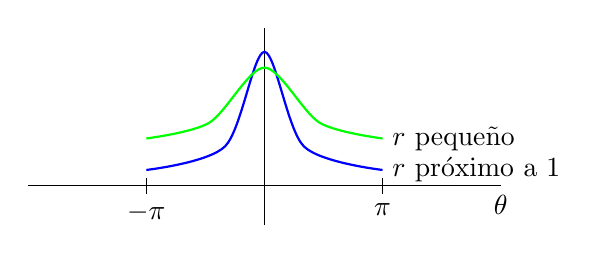
\begin{tikzpicture}

			\draw[-] (-3,0) -- (3,0) node [below] {$\theta$};
			\draw[-] (0,-0.5) -- (0,2);

			\draw[-] (-1.5,0.1) -- (-1.5,-0.1) node[below] {$-\pi$};
			\draw[-] (1.5,0.1) -- (1.5,-0.1) node[below] {$\pi$};

			\draw[blue, thick] plot[smooth] coordinates {(-1.5,0.2) (-0.5,0.5) (0,1.7) (0.5,0.5) (1.5,0.2)};

			\draw[green, thick] plot[smooth] coordinates {(-1.5,0.6) (-0.7,0.8) (0,1.5) (0.7,0.8) (1.5,0.6)};

			\node[right] at (1.5,0.6) {$r$ pequeño};
			\node[right] at (1.5,0.2) {$r$ próximo a 1};

			\end{tikzpicture}
			\end{center}

			Puesto que la función es periódica da lo mismo integrar entre $-\pi$ y $\pi$ que cualquier otro intervalo de tamaño $2\pi$. Todas serán 1.

		\end{itemize}

		\begin{theorem} \label{thm:ConvUniformePoisson}
			Supongamos que $g$ es una función continua y $2\pi$-periódica. Entonces:

			\[ \int^\pi_{-\pi} g(s)P(r, \theta-s) \dif s \convs[][r][1^-] g(\theta) \text{ uniformemente en } [-\pi,\pi] \]

			IMPORTANTE: Este es el primer teorema que vemos en el que se nos indica el límite a parte de darnos convergencia uniforme. Usaremos este teorema como base para ampliar los resultados anteriores.
		\end{theorem}

			\begin{proof}
				Para hacer la prueba vamos a estimar la diferencia entre ambas funciones:
				\[0 \leq \left| \int_{-\pi}^{\pi} g(s) P(r, \theta-s) \dif s  - g(\theta))  \right| \]

				Tenemos que $\int_{-\pi}^{\pi} P(r, \theta-s) \dif s = 1$, luego podemos meterlo dentro multiplicando a $g(θ)$ sin que nada cambie:
				\begin{align*}
				0	&≤ \left| \int_{-\pi}^{\pi} g(s) P(r, \theta-s) \dif s - g(\theta) \int_{-\pi}^{\pi} P(r, \theta-s) \dif s  \right| = \\
					&= \left| \int_{-\pi}^\pi (g(s) - g(\theta)) P(r, \theta - s) \dif s \right|
					≤ \int^{\pi}_{-\pi} | g(s) - g(\theta) | P(r, \theta- s)
				\end{align*}

				Hemos podido hacer este paso ya que $P>0$, pero veremos en unos días que no se va a cumplir en otra prueba y tendremos problemas.

				Vamos a descomponer la integral en dos trozos, en uno nos ayudaremos de la continuidad de $g$ y en el otro de la del núcleo.

				\[ = \underbrace{\int_{|\theta-s|< \delta}}_{|g(s) - g(\theta)| \text{ pequeño y }P\text{ grande}} + \underbrace{\int_{|\theta-s| > \delta}}_{|g(s) - g(\theta)| \text{ acotado y }P\text{ pequeño}} \]

				\proofpart{Primera integral, en $\abs{θ - s} < δ$}

				Para la primera integral, sabemos que $g$ es continua en $[-\pi,\pi]$, intervalo cerrado y acotado. Como $[-\pi,\pi]$ es compacto, entonces $g$ es uniformemente continua\footnote{Igual que la continuidad normal con la definición $ε-δ$, salvo porque el $δ$ no depende del punto que consideremos y nos vale para todo el intervalo. En este caso, como $g$ es continua en un compacto, para cada ε podemos tomar el δ máximo para cada punto, que existe y está bien definido.}.

				Dado $\epsilon > 0$, $\exists \delta > 0$ tal que si $|\theta-s| < \delta$, entonces $|g(s) - g(\theta)| < \epsilon, \forall \theta ∈ [-π, π]$. Así, podemos estimar la integral fácilmente:
				\[
					\int\limits_{|\theta - s| < \delta} \abs{g(s) - g(\theta)} P(r, \theta - s) \dif s < \epsilon \int\limits_{|\theta - s| < \delta} P < \epsilon \int_{-\pi}^{\pi} P = ε
				\]

				Luego tiende a 0, pero hay que tener cuidado porque ya hemos dejado fijado $\delta$.

				\proofpart{Segunda integral, en $\abs{θ - s} > δ$}

				Para el delta elegido en la integral anterior podemos dividir la integral en dos partes: \begin{multline*}
				\int\limits_{|\theta - s | > \delta} \abs{g(s) - g(\theta)} P(r, \theta-s) \dif s = \\
				= \int_{\theta+\delta}^\pi \underbrace{|g(s) - g(\theta)| P(r, \theta-s) \dif s}_{(A)} +  \int_{-\pi}^{\theta-\delta} \underbrace{|g(s) - g(\theta)| P(r, \theta-s) \dif s}_{(B)}
				\end{multline*}

				Y tenemos:

				\[ (1) \leq P(r, \theta-(\theta-\delta)) = P(r, -\delta) = P(r, \delta) \leq  \]

				\[\leq P(r, \delta) \int^{\pi}_{\theta+\delta} |g(s) - g(\theta) ds \leq C P(r, \underbrace{\delta}_{> 0}) \convs[][r][1^-] 0  \]

				\[g \text{ continua } \Rightarrow |g| < M \]

				\[ |g(s)  - g(\theta)| \leq |g(s)| + | g(\theta) | \leq 2M \]


				Hemos probado:

				Dado $\epsilon > 0$, $\exists r_0$ tal que si $r \in (r_0,1)$:

				\[ \left| \int_{-\pi}^\pi g(s) P(r, \theta-s) ds - g(\theta)  \right| < \epsilon \quad \forall \theta \]

			\end{proof}

		La primera aplicación que nos da este teorema es muy sencilla y algo esperable: si tenemos dos funciones $f,g$ continuas con los mismos coeficientes de Fourier, entonces son la misma función\footnote{Misma función \textit{en $L^2$}, que es un detalle sutil. En $L^2$, dos funciones son equivalentes si y sólo si son iguales en casi todo punto. Es decir, que $f$ y $g$ podrían ser distintas, aunque sólo en un conjunto de medida cero.}.

		\begin{proof}
			\[
				\left. \begin{array}{l}
				f \\
				g
				\end{array} \right\} \rightarrow \alpha_k \rightarrow \sum_k \alpha_k r^{|k|} e^{ik\theta} \left\{ \begin{array}{l}
					\int^{\pi}_{-\pi} f(s) P(r, \theta - s)ds \convs[][r][1^-] f \\
					\int^{\pi}_{-\pi} g(s) P(r, \theta - s)ds \convs[][r][1^-] g
				\end{array} \right.
			\]

			Por unicidad del límite $\Rightarrow f \equiv g$
		\end{proof}

		% clase 2016/02/29

		Si tenemos un problema en una circunferencia de radio $a$, hacemos un reescalado:

		% faltan tildas aquí, que no he sabido ponerlas durante la clase
		\[ \gor{W}(\rho, \theta) = W(\frac{\rho}{a},\theta) \quad \rho \in [0,a) \]

		Usando la regla de la cadena llegamos a:

		\[\gor{W}_{\rho \rho} + \frac{1}{\rho} \gor{W}_\rho + \frac{1}{\rho^2} \gor{W}_{\theta \theta} = 0, \quad \rho \in [0,a)  \]

		\[\gor{W}(\rho, \theta) = W(\frac{\rho}{a},\theta) = \int^{\pi}_{-\pi} g(s)\underbrace{P(\frac{\rho}{a},\theta-s)}_{\text{núcleo de Poisson para la bola de radio }a} ds \]

		Ya como consecuencias algo más interesantes del teorema de Poisson tenemos las siguientes proposiciones.

		\begin{prop}[Propiedad\IS de la media]

		 \[u(x,y)|_{(0,0)}  = W(0,\theta) = \int_{-\pi}^\pi g(s) P(0, \theta - s) ds = \frac{1}{2\pi} \int_{-\pi}^\pi g(s) ds \]

		 \[ u_{xx} + u_{yy} = 0\]
		\end{prop}

		 Las funciones que verifican la condición de Laplace (las funciones armónicas) son muy rígidas y verifican que son el promedio de todos los puntos de la circunferencia que les rodea. Son las funciones que aparecen en los equilibrios, por ejemplo, en la función de ondas.

		Lo veremos más adelante, pero se puede imaginar una membrana, que cuando se queda parada, en una posición de equilibrio, los puntos interiores dependen de la forma del bastidor que sujeta la membrana.

		\begin{prop}[Propiedad\IS del máximo]
		Si $m \leq g(\theta) \leq M, \forall \theta \in [-\pi,\pi]$, entonces $m \leq u(x,y) \leq M, \forall (x,y)$

		\[u(x,y) \rightarrow W(r,\theta) = \int_{-\pi}^{\pi} \underbrace{g(s)}_{\in [m,M]} \underbrace{P(r,\theta-s)}_{> 0} ds \begin{cases}
			\leq \int_{-\pi}^{\pi} MP = M \\
			\geq \int_{-\pi}^{\pi} mP = m

		\end{cases} \]

		Una función armónica alcanza mínimo y máximo en el borde, no puede alcanzarlo en el interior.
		\end{prop}

		\textbf{iii:} $f$,$g$ contínuas, $2\pi$-periódicas si:

		\[ \int_{-\pi}^{\pi} f(s) e^{-iks}ds =
		 \int_{-\pi}^{\pi} f(s) e^{-iks}ds,  \forall k \Rightarrow f \equiv g \]

		\begin{theorem}[Teorema\IS de aproximación de Weirestrass (I)] \label{thm:AproxWeierstrass1} Sea $f$ contínua y $2\pi$-periódica. Entonces existe un polinomio trigonométrico:

		\[T_n (\theta) = \sum_{k = -n}^n c_k e^{ik\theta} \]

		tal que $\forall \epsilon > 0$ existe $n_0$ tal que si $n > n_0$: $|T_n (\theta) - f(\theta)| < \epsilon, \forall \theta \in [-\pi,\pi]$.
		\end{theorem}

		\begin{proof}

			\[f \rightarrow \alpha_k = \int_{-\pi}^\pi f(s) e^{-iks} ds  \]

			\[ \sum_{k=-\infty}^{\infty} \alpha_k r^{|k|} e^{ik\theta} \convs[][r][1^-] f(\theta), \text{ uniformemente.} \]

			Dado $\epsilon > 0$, $\exists \delta > 0$ tal que si $1-\delta < r < 1$ entonces:

			\[ \left| \sum_{k=-\infty}^{\infty} \alpha_k r^{|k|} e^{ik\theta} - f(\theta) \right| < \epsilon, \forall \theta \in [-\pi,\pi]  \]

			Fijamos $r_{*} \in (1-\delta, 1)$

			\textbf{a}

			\[ \left| \sum_{k=-\infty}^{\infty} \alpha_k r^{|k|} e^{ik\theta} - f(\theta) \right| < \epsilon \]

			\[  r_* < 1 \Rightarrow \sum_{k=-\infty}^\infty \alpha_k r_*^{|k|} e^{ik\theta} < \infty \eqreason[\Rightarrow]{Dado $\epsilon > 0, \exists N_0$ tal que si $n \geq n_0$} \sum_{|k| > n} \alpha_k r_*^{|k|} e^{ik\theta} < \epsilon \]

			\textbf{a,b}

			\[ \Rightarrow  \left| \underbrace{\sum_{|k| < k} \alpha_k r_*^{|k|} e^{ik\theta}}_{\text{Suma finita (polinomios trigonométricos)}} - f(\theta) \right| < 2 \epsilon, \forall \theta \in [-\pi,\pi] \]

			Por lo tanto cualquier función contínua se puede aproximar uniformemente por una suma finita de $\alpha_k r^{|k|_* e^{ik\theta}}$.

		\end{proof}

		\begin{theorem}Teorema\IS de aproximación de Weirestrass (II)] \label{thm:AproxWeierstrass2}
		Dada una función $f$ $2\pi$-periódica y continua. $\forall \epsilon > 0 \exists$ un polinomio $p(x)= a_0 + a_1 x + … + a_n x^n $ tal que $|f(x)-P(x)| < \epsilon, \forall x \in [-\pi,\pi]$
		\end{theorem}

		\begin{proof}
			Usar la misma prueba que con el primer teorema de aproximación de Weirestrass
		\end{proof}

		Con esto llegamos a la idea de que si la función $f$ fuera analítica tendríamos que se aproxima uniformemente en un intervalo por su polinomio de Taylor (como los senos y los cosenos).

		Si aproximamos una función con un polinomio trigonométrico, entonces lo tenemos aproximado por muchos términos con senos y cosenos, lo cual son funciones analíticas, que permiten aproximar cada uno de ellos a su polinomio de Taylor del orden que se quiera. Si acotamos cada término con ($\epsilon / $ número de términos) entonces el error total será menor a $\epsilon$.

		Tenemos el problema de que no nos dice como calcular ese $p(x)$, la prueba no es constructiva. Sin embargo, el teorema de funciones analíticas si te da esa solución, pero solo vale para funciones iguales a su polinomio de Taylor.

		\subsection{Identificación del límite con convergencia $L^2$}
		\textbf{Aplicación} al estudio de la convergencia en $L^2$.

		\begin{theorem} \label{thm:ConvergenciaL2}
			Partimos de $\{\Phi_k\}$, con $\Phi_k(s) = \frac{e^{iks}}{\sqrt{2\pi}}$, un sistema ortonormal en $L^2([-\pi,\pi])$ y $f \in L^2$, con los coeficientes de Fourier
			\[\alpha_k = \pesc{f, \Phi_{k}} = \int_{-\pi}^\pi f(s) \overline{\Phi_k(s)} \dif s  \] y las sumas parciales
			\[  S_n f = \sum_{|k| < n} \alpha_k · \Phi_k = \sum_{|k| < n}\pesc{f, \Phi_k} \Phi_k \]

			Entonces, para todo $ε > 0$ podemos encontrar $T_n$ polinomio trigonométrico de grado $n$, tal que
			\[ \| S_n f - f\|_{L^2} \leq \| T_n - f \|_{L^2} < \epsilon \]

			La igualdad se dará sólo si $S_n \equiv T_n$.

		\end{theorem}

			\begin{proof}

				\[ T_n = \sum_{|k| < n} C_k \Phi_k(x) \]

				\[ \| T_n - f \|_{2}^2 = < T_n -f, T_n - f> = < \sum_{|k| < n} C_k \Phi_k(x) - f, \sum_{|k| < n} C_k \Phi_k(x) - f >   \]

				\begin{align*} = < &\sum_{|k| < n} C_k \Phi_k(x), \sum_{|j| < n} C_j \Phi_j(x) > - < \sum_{|k| < n} C_k \Phi_k(x), f> \\ &- <f, \sum_{|j| < n} C_j \Phi_j(x)> + <f,f> \end{align*}

				\[ = \sum_{|k| < n} C_k^2 - \sum_{|k| < n} C_k <\Phi_k(x),f> - \sum_{|j| < n} C_j <\Phi_j(x),f> + \|f\|_2^2  \]


				\[ \| S_n f - f \|_2^2 = … = < \sum_{|k| < n} <f,\Phi_k(x)> \Phi_k -f,  \sum_{|j| < n} <f,\Phi_j(x)> \Phi_j -f>\]

				\[ = … = \|f\|_2^2 - \sum_{|k| < n} |<f,\Phi_k(x)>|^2 \]

				Entonces:

				\[ \| S_n f - f \|_2^2 - \|T_n -f\|_2^2 = … = \sum_{|k| < n} \underbrace{(<f,\Phi_k> - C_k) \overline{(<f,\Phi_k> - C_k)}}_{|<f, \Phi_k> - C_k|^2 < 0}  \]


			\end{proof}

		\textbf{Consecuencias:}

		\begin{itemize}

			\item  \[ f \in L^2 \Rightarrow S_n f \eqexpl[\rightarrow]{$L^2$} f \]

			Lo cual es consecuencia de l resultado anterior junto con el primer teorema de aproximación de Weirestrass

			\item \[ \| S_n f - f \|_{2}^2 - \sum_{|k|<n} | <f, \Phi_k> |^2  \]

			Entonces obtenemos la \concept{Identidad\IS de Parseval}:

			\[ \sum_{k= -\infty}^\infty  |\pesc{f, \Phi_k}|^2 = \|f\|^2_2 \]


		\end{itemize}

		% Revisado hasta aquí

		%clase 2016/03/01


		Aunque hemos hecho trampa, porque hemos aplicado un resultado válido solo para funciones contínuas a funciones que no sabíamos si lo eran. El siguiente teorema nos ayudará con ello:

		\begin{theorem} \label{thm:ConvergenciaL2Limite}

			\[ f \in L^2 \Rightarrow S_n f \eqexpl[\rightarrow]{$L^2$} f \]

		\end{theorem}

		\begin{proof}

			\textbf{Caso 1:} Supongamos $f$ contínua.

			Por Weierstrass tenemos que dado $\epsilon > 0$, existe un polinomio $T_n$ tal que $|T_n(s) - f(s)| < \epsilon, \forall s \in [-\pi,\pi]$

			\(
				\int^{\pi}_{-\pi} | S_n f - f |^2 ds \leq \int^\pi_{-\pi} | T_n - f |^2 ds < 2 \pi \epsilon^2 \label{eq:resultadoContinuidadWeierstrass}
			\)

			\textbf{Caso 2:} $f \in L^2 ([-\pi,\pi])$

			Recordemos las dos definiciones equivalentes de $L^2$:
			\begin{itemize}

				\item $L^2 \equiv$ funciones medibles tales que $\int\limits^\pi_{-\pi} |f|^2 dx \leq \infty $

				\item $L^2 \equiv$ cierre del conjunto de las funciones contínuas con la topología inducida por $\|\cdot\|_2$, que se relaciona con \ref{eq:resultadoContinuidadWeierstrass}

			\end{itemize}

			Data $f\in L^2, \exists \set{f_n}$ de funciones contínuas tales que $\|f_n - f\|_2 \convs 0$

			Sea $f_\epsilon$ contínua con $\|f-f_\epsilon\|_2 < \epsilon$:

			Entonces,
			\begin{align*}
			\| S_N f - f \|_2 &= \| S_N f \pm S_N f_\epsilon \pm f_\epsilon - f \|_2 \leq \\
			& \leq \| S_N f - S_N f_\epsilon \|_2 + \| S_N f_\epsilon - f_\epsilon \|_2 + \underbrace{\| f_\epsilon - f \|_2}_{< \epsilon}
			\end{align*}

			Tenemos que $\| S_N f_\epsilon - f_\epsilon \|_2 \convs 0$ por el caso 1; y

			\[ \| S_N f - S_N f_\epsilon \|_2 \eqreason{sumas finitas} \| S_N (f - f_\epsilon) \|_2 \eqreason[\leq]{Bessel} \| f - f_\epsilon \|_2 \]

			Luego tenemos que $\| S_N f - f \|_2 < \epsilon$.

		\end{proof}

		\begin{corol}

		\[ \| S_n f - f \|_2^2 = \|f\|_2^2 - \sum_{-n}^{n} |<f, \Phi_k>|^2\]

		\[\rightarrow \|S_n f - f \|_2 \convs 0 \]

		\[\Rightarrow  \sum_{-\infty}^{\infty} | <f, \Phi>|^2 \eqreason{Parçeval} \|f\|_2^2 \]

		con $\{\Phi_k\}$ ortonormal. Esta fórmula nos permite calcular sumas infinitas.

		\end{corol}


	\subsection{Resultados probados}


		\begin{itemize}

			\item $f \in C^2, 2\pi$-periódica $\Rightarrow S_n f \rightarrow f$ uniformemente

			\item $f\in L^2 \Rightarrow S_n f \eqexpl[\rightarrow]{$L^2$} f$

			\item Bessel, Parseval

			\item Convergencia uniforme de la ``serie modificada'' $\sum\limits_k \alpha_k r^{|k|} e^{ikx}$ (Poisson)

		\end{itemize}


	\subsection{Convergencia puntual}

	\begin{theorem}[Teorema\IS de Dirichlet]

		\[ \{\Phi_k\} = \set{\frac{1}{\sqrt{2\pi}} e^{ikx}}_{k=0, ±1,±2}  \text{ es  un sistema ortonormal en } [-\pi,\pi]\]

	\end{theorem}

	\begin{proof}

		f ``regular''

		\[S_nf = \sum_{k=-n}^{n} <f,\Phi_k> \Phi_k(x) = \sum_{-n}^n \left( \int_{-\pi}^\pi f(s) \frac{1}{\sqrt{2\pi}} e^{-iks} ds \right)  \frac{1}{\sqrt{2\pi}} e^{ikx} \]

		\[ = \sum_{-n}^{n}  \int_{-\pi}^\pi f(s) \frac{1}{2\pi} e^{-ik(s-x)} ds = \int_{-\pi}^{\pi} f(s) \frac{1}{2\pi} \sum_{-n}^n e^{-ik(s-x)} ds \]

		Continuamos con solo el sumatorio de la ecuación anterior: es una progresión geométrica, así que la sabemos calcular (salvo en el límite):

		\[ \frac{1}{2\pi} \sum_{-n}^n e^{-ik(s-x)} = \frac{1}{2\pi} \sum_{-n}^n e^{ik(x-s)} = \frac{1}{2\pi} \sum_{-n}^n \left[\underbrace{e^{i(x-s)} }_{\equiv \rho}\right]^k \]

		\[ \frac{1}{2\pi} \sum_{-n}^n \rho^k = \frac{1}{2\pi} \frac{\rho^{-n} - \rho^{n+1}}{1 -\rho} \]

		\begin{gather*}
		\frac{1}{2\pi}  \sum(e^{it})^k = \frac{1}{2\pi} \frac{e^{-nit}-e^{(n+1)it}}{1-e^{it}} = \frac{1}{2\pi} \frac{e^{-it/2}}{e^{-it/2}} \frac{ e^{-nit}-e^{(n+1)it}}{1-e^{it}} =\\
		= \frac{1}{2\pi} \frac{e^{-(n + 1/2)it}-e^{(n+1/2)it} }{e^{-it/2}-e^{it/2}} \cdot \frac{-1}{-1} = \frac{1}{2\pi} \frac{e^{(n + 1/2)it} - e^{-(n+1/2)it} }{e^{it/2}-e^{-it/2}} = \dots
		\end{gather*}

		\( … = \frac{1}{2\pi} \frac{\sin(n+ \frac{1}{2})t}{\sin(\frac{t}{2})}  \equiv D_n(t) \label{eq:nucleoDirichlet}\)
	\end{proof}

		La expresión \ref{eq:nucleoDirichlet} que hemos obtenido es conocida como \concept{Núcleo\IS de Dirichlet}.

		Pero nos falta por estudiar cuál es la relación entre las propiedades del núcleo de Dirichlet cuando n tiende a infinito y el límite de $S_N f$.



	\begin{figure}[hbtp]
	\centering
	\inputtikz{PoissonDirichlet}
	\caption{Núcleo de Poisson $P(s,t)$ (verde)  y de Dirichlet $D_n(t)$ (naranja). Gráfica más oscura implica valores mayores de $s$ y $n$ respectivamente.}
	\label{fig:PoissonDirichlet}
	\end{figure}

	En la \fref{fig:PoissonDirichlet} comparamos los núcleos de Poisson y Dirichlet. Como podemos ver, Dirichlet plantea problemas de convergencia.

	El argumento que debemos utilizar debe basarse en las oscilaciones, ya que no tenemos nada más que nos lo permita. Tendremos una integral que queremos hacer tender a cero por culpa de las oscilaciones por culpa de las oscilaciones de dentro, sin tener que meter valor absoluto. El teorema que nos da este tipo de argumentos es el de Riemann-Lebesgue.Veamos:

	Fijando x:

	\( |S_n f(x) - f(x) | = \left| \int_{-\pi}^\pi f(s) D_n (x-s) ds - f(x) \right| \label{eq:dirichletFijandoX} \)

	\textbf{propiedades de $D_n$:}

	\begin{itemize}
		\item $D_n(-t) = D_n(t)$

		\item $\int\limits_{-\pi}^{\pi} D_n(t) = 1, \forall n $

		\[ \int_{-\pi}^\pi  \frac{1}{2\pi} \sum_{-n}^{n} e^{ikt} dt \]

	\end{itemize}


	Entonces:

	\[  \int_{x-\pi}^{x +\pi} f(x-t) D_n(t) dt = \int^{\pi}_{-\pi} f(x-t) D_n(t) dt \]

	\[ \eqref{eq:dirichletFijandoX} = \left| \int_{-\pi}^\pi (f(x-t)-f(x)) \frac{1}{2\pi} \frac{\sin(n+\frac{1}{2})t}{\sin{\frac{t}{2}}} dt \right| \]

	% clase 7/3/2016

	\begin{theorem}[Teorema\IS de convergencia puntual de Dirichlet (1)] \label{thm:Dirichlet1}
		Sea $f$ medible y acotada derivable en $x$. Entonces $S_n f(x) \convs f(x)$.
	\end{theorem}

	\begin{proof}

		\[ 0 \leq |S_nf(x) - f(x)  = \left| \int_{-\pi}^{\pi} f(x-t) D_n(t) dt - f(x) \int_{-\pi}^\pi D_n(t) dt \right|  \]

		\[= \left| \int_{-\pi}^\pi (f(x-t)-f(x) D_n(t) dt) \right| = \frac{1}{2\pi} \left| \int_{-\pi}^\pi \frac{f(x-t)-f(x)}{\sin t/2} \frac{\sin(\pi+1/2)t}{\sqrt{\pi}} \right|  \]

		Utilizamos dos teoremas para completar la demostración:

		\begin{itemize}

			\item \textbf{Teorema 1:} $\frac{1}{\sqrt{\pi}} \sin(n + \frac{1}{2}) t $ es una familia ortonormal en $[-\pi,\pi]$

			La demostración se deja como ejercicio al lector

			\item \textbf{Teorema 2:}  En las hipótesis del teorema:

			\[ \frac{f(x-t)-f(x)}{\sin(t/2)} \eqreason[\in]{variable $t$, ($x$ fijo)} L^2 ([-\pi,\pi]) \]

			\begin{proof}
				Sea
				\[ g(t) = \frac{f(x-t)-f(x)}{\sin(t/2)} = \underbrace{\frac{f(x-t)-f(x)}{-t}}_{\convs[ ][t][0] f'(t)} \underbrace{\frac{-t}{\sin(t/2)}}_{\convs[ ][t][0] 2} \]
				Entonces existe un $\delta > 0$ tal que $\| g(t) \| < C$, si $\| t \| < \delta$.

				Observemos que el seno entre $-\pi$ y $\pi$ es impar, y que si quitamos una bola entrada en el 0 de radio $\delta$ tenemos que $\| \frac{1}{\sin(t/2)} \| < k$, si $\| t \| < \delta$.

				Como f es derivable y tenemos un intervalo acotado, tenemos que f está acotada, luego $\| f(x-t) - f(x) \| \leq 2 M$.

				Por tanto, $\| g(t) \| < \gor{C}$, $\forall t \in [-\pi,\pi]$.

				Finalmente,
				\[ \int\limits_{-\pi}^{\pi} \| g(t) \|^2 dt < 2M \gor{C} \implies g \in L^2 \]
			\end{proof}

		\end{itemize}

		Conclusión:

		Lema 1 + Lema 2 + Riemman-Lebesgue $\Rightarrow \left| S_n f(x) - f(x) \right| \rightarrow 0$

	\end{proof}

	\begin{theorem}[Teorema\IS de convergencia puntual de Dirichlet (2)] \label{thm:Dirichlet2}

		$f$ medible y acotada. Además solo vamos a permitir discontinuidades de salto, dientes de sierra, etc.. pero vamos a evitar funciones con derivadas infinitas en algún punto. Admitimos límites y derivadas laterales siempre que sean finitos:

		{\inputtikz{FuncionesDirichlet}}

		\[
		\left.
		\begin{array}{l}
			f(x^+) = \lim_{t \to x^+} f(t) \\
			f(x^-) = \lim_{t \to x^-} f(t) \\
			f'(x^+) = \lim_{h \to 0^+} \frac{f(x+h)-f(x)}{h} \\
			f'(x^-) = \lim_{h \to 0^-} \frac{f(x+h)-f(x)}{h}
		\end{array} \right\} \text{ existen y son finitos.}
		\]

		Entonces: \[ \lim_{n \to \infty} S_nf(x) = \frac{1}{2} \{f(x^+)+f(x^-)\}\]

	\end{theorem}

	\begin{proof}

		\[ 0 \leq | S_n f(x) - \frac{1}{2} \{f(x^+) + f(x^-)\} |\]

		\[ = \left| \int_{-|pi}^\pi f(x-t) D_n (t) dt - \frac{1}{2} f(x^+)- \frac{1}{2} f(x^-) \right|  \]

		\[ \int_{-|pi}^{0} f(x-t) D_n(t)dt + \int_{0}^\pi f(x-t) D_n(t) dt \]

		\[ \left| \underbrace{\int_0^\pi  \{ f(x-t) - f(x^+) \} D_n(t) dt }_{\text{I}} + \underbrace{\int_{-\pi}^{0}  \{ f(x-t) - f(x^-) \} D_n(t) dt }_{\text{II}} \right| \]

		\[\leq | \text{I} | +  |\text{II}| \]

		Si nos fijamos en I:

		\[ I = \frac{1}{2\sqrt{\pi}} \int_{0}^\pi \underbrace{\frac{f(x-t)-f(x)}{\sin(t/2)}}_{=g(t)} \cdot \frac{\sin((n+1/2)t)}{\sqrt{\pi}} \]

		Ojo, $\frac{\sin((n+1/2)t)}{\sqrt{\pi}}$ es un sistema ortonormal en $[-\pi,\pi]$, pero no es siquiera ortogonal en $[0,\pi]$.

		Tenemos
		\[ \int_{0}^\pi \underbrace{g(t)}_{\in L^2} \underbrace{\sin((n+1/2)t)}_{\text{impar}} dt \]
		y lo que debemos hacer es extenderla a $[-\pi,\pi]$.

		Consideramos una función $\gor{g}$, que será la extensión IMPAR de $g$ en el intervalo $[-\pi,\pi]$. Entonces:

		\[ \int_{-\pi}^\pi  \gor{g}(t) \sin(n+1/2)t dt \eqreason[\rightarrow]{Riemann-Lebesgue} 0 \]

		\[ = 2 \int_{0}^\pi g(t) \sin(n \frac{1}{2}) t dt \]


	\end{proof}


	\begin{example}

		Dada $f(x) = x(\pi-x), x \in [0,\pi]$

		(DIBUJO SEMICIRCUNFERENCIA).

		\textbf{1:}

		$f_1 = $ extensión par de $f$:

		(DIBUJO)

		\[\{ 1, \sin{kx}, \cos{kx} \}_{K = ±1,±2,…} \]

		\obs No está normalizada, si quisiéramos usar Parseval, tendríamos que normalizar.

		El teorema de Dirichlet nos garantiza lo siguiente:

		\[
			f_1(x) = \frac{a_0}{2} + \sum_{k=1}^\infty a_k \cos{kx} + \sum_{k=1}^\infty b_k \sin kx
		\]

		Pero tenemos que $b_k = 0 \forall x$:

		\[b_k = \frac{1}{\pi} \int_{-\pi}^{\pi} f_1(x) \sin kx dx = 0 \]

		Tenemos que $a_0$ es:

		\[ a_0 = \frac{1}{\pi} \int_{-\pi}^{\pi} f_1(x) dx = … = \frac{\pi^2}{3} \]

		\[ a_k = \frac{1}{\pi} \int_{-\pi}^{\pi} \underbrace{f_1(x) \cos (kx)}_{\text{par}} dx = \frac{2}{\pi} \int_{0}^{\pi} x(\pi - x) \cos (kx) dx \]

		\[ = \frac{2}{\pi} \left\{ \pi \int_{0}^{\pi} x \cos(kx) dx  - \int_{0}^{π} x^2 \cos(kx) dx \right\} = \text{ por partes dos veces ...} \]

		\[ \Rightarrow … \Rightarrow a_k = \begin{cases}
			\frac{-4}{k^2} & k \text{ par} \\
			0 & k \text{ impar}
		\end{cases}  \]

		Luego tenemos que $\frac{a_0}{2} = \frac{\pi^2}{6}$ y $a_{2n} = \frac{-4}{(2n)^2} = \frac{-1}{n^2}$

		\obs si hacemos una extensión {\bf par}, tendrá periodo $\pi$; y si hacemos una extensión {\bf impar} tendrá periodo $2\pi$.

		{\bf Conclusión:}

		\[ x(\pi - x) = \frac{\pi^2}{6} -\sum_{n=1}^{\infty} \frac{1}{n^2} \cos(2n x) \]

		En particular, si $x=0$:

		\[ 0 = \frac{π^2}{6}  - \sum_{n=1}^\infty \frac{1}{n^2} \Rightarrow  \sum_{n=1}^\infty \frac{1}{n^2} = \frac{\pi^2}{6} \]

		Este resultado fue probado por Euler, y la suma de $\frac{1}{n^2}$ se la conoce como \concept{Problema de la suma de Basilea}.

		Lo más interesante es que a partir de ésta, Euler pudo calcular otras series, por ejemplo:
		\begin{gather*}
			\frac{\pi^2}{6} = \sum_n \frac{1}{n^2} = \sum_{n \text{ par}} \frac{1}{n^2} + \sum_{n \text{ impar}} \frac{1}{n^2} =\\
			= \sum_{j=1}^\infty \frac{1}{(2j)^2} + \sum_{j=1}^\infty \frac{1}{(2j-1)^2} = \frac{1}{4} \underbrace{\sum_{j=1}^\infty \frac{1}{j^2}}_{= \frac{\pi^2}{6}} \ + \ \sum_{j=1}^\infty \frac{1}{(2j-1)^2}
		\end{gather*}

		Despejando obtenemos que
		\[ \sum_{j=1}^\infty \frac{1}{(2j-1)^2} = \frac{\pi^2}{6} - \frac{1}{4} \frac{\pi^2}{6} = \frac{\pi^2}{8} = 1 + \frac{1}{3^2} + \frac{1}{5^2} + … \]

		\textbf{2:}

		Veamos $f_2$ como la extensión impar de $f$:

		(DIBUJO)

		\[ f_2 \Rightarrow \underbrace{\frac{a_0}{2}}_{0} + \sum_k \underbrace{a_k \cos(kx)}_{0} + \sum_k b_k \sin(kx)  \]

		\[  x(\pi - x) = \sum_{n=1}^{\infty} \frac{8}{n(2n-1)^3} \sin(2_n-1)x  \]

		\[  1 - \frac{1}{3^3} + \frac{1}{5^3} - \frac{1}{7^3} + … = \frac{\pi^3}{32}\]


	\end{example}








% Clase 8/3/2016

Al igual que con el teorema de Dirichlet, podemos ver la aplicación de la identidad de Parçeval, que nos decía que \[ \norm{f}_{L^2}^2 = \sum_{k ∈ ℤ} \abs{\pesc{f, φ_k}}^2 \] con $\set{φ_k}$ nuestro sistema ortonormal.

Consideramos de nuevo la extensión par de $f(x) = x(π-x)$. Podemos calcular y ver que \[ \pesc{\tilde{f}, φ_0} = \frac{1}{\sqrt{2π}} 2 \int_0^π x(π-x) \dif x = \sqrt{\frac{2}{π}} \left(\frac{πx^2}{2} - \frac{x^3}{3}\right|_{x = 0}^π =  \sqrt{\frac{2}{π}} \frac{π^3}{6} \]

Para el resto de los coeficientes, vemos primero que los coeficientes de los senos van a ser $0$ por simetría. En el caso de los cosenos, vemos que \[ \pesc{\tilde{f}, \frac{\cos kx}{\sqrt{π}}} = \frac{2}{\sqrt{π}} \int_{0}^π x(π-x) \cos kx \dif x = \frac{2}{\sqrt{π}} \left(π\int_0^π x \cos kx \dif x - \int_0^π x^2 \cos kx \dif x \right) \]

Resolvemos las dos integrales por separado: \[ \int_0^π x \cos kx \dif x = x \eval{\frac{\sin kx}{k}}_{x=0}^π - \int_0^π \frac{\sin kx}{k} \dif x = \eval{\frac{\cos kx}{k^2}}_{x=0}^π = \frac{(-1)^k - 1}{k^2} \] y la otra integral sale \[ \int_0^π x^2 \cos kx \dif x = \dotsb = \frac{2π}{k^2} (-1)^k \]

Juntando ahora y haciendo más cuentas, queda que \[ \pesc{\tilde{f}, \frac{\cos kx}{\sqrt{π}}} = \frac{2 \sqrt{π}}{k^2}\left(-1 - (-1)^k\right) = \frac{2\sqrt{π}}{k^2} \begin{cases} 0 & k \text{ impar} \\ -2 & k \text{ par} \end{cases} \]

Por otra parte, vemos que \[ \norm{\tilde{f}}^2_{L^2} = \dotsb =\frac{π^5}{15} \]

Así, la identidad de Parçeval nos dice que \[ \frac{π^5}{15} = \left(\sqrt{\frac{2}{π}} \frac{π^3}{6}\right)^2 + \sum_{n=1}^∞ \left(\frac{2\sqrt{π}}{(2n)^2} - ( -2)\right)^2 = \frac{π^5}{18} + \sum_{n=1}^{∞} \frac{π}{n^4} \] y que simplificando \[ \sum_{n=1}^∞ \frac{1}{n^4} = \frac{π^4}{90} \]

Incluso podríamos repetir el resultado que hacíamos antes y sacar todavía más resultados de teoría de números, separando la suma de los pares y los impares \[ \frac{π^4}{90} = \sum_{k ∈ ℕ} \frac{1}{(2k)^4} + \sum_{k ∈ ℕ} \frac{1}{(2k-1)^4} = \sum_{k∈ℕ} \frac{1}{16k^4} + \sum_{k ∈ ℕ} \frac{1}{(2k-1)^4} \] y entonces podemos despejar y ver que \[ \sum_{k ∈ ℕ} \frac{1}{(2k-1)^4} =  \frac{π^4}{90} \frac{15}{16} \]


\subsection{Convergencia puntual para funciones Hölder continuas}

Recuperando lo que teníamos antes, teníamos que la continuidad no nos bastaba para tener convergencia de la serie de Fourier. Du Bois-Raymond construía un ejemplo de una función continua cuya serie no convergía en un punto, y Kolmogorov iba un poco más allá con una función continua cuya serie divergía en todo punto.

Pediremos algo más que continuidad:

\begin{defn}[Función\IS continua Hölder]\label{def:FuncContinuaHolder} Se dice que una función $\appl{f}{X}{ℝ}$ es Hölder continua si existe un $α ∈ [0,1]$ y $K ∈ ℝ$ tal que $∀t,s ∈ X$ (por ejemplo, $X = [-π, π]$) se cumple que \[ \abs{f(t) -f(s)} < K \abs{t-s}^α\]
\end{defn}

\begin{theorem} \label{thm:ConvPuntualHolder} Sea $\appl{f}{X}{ℝ}$ una función Hölder continua. Entonces su serie de Fourier converge en todo punto a $f(x)$.
\end{theorem}

El punto de partida es el de siempre: tenemos que \[ \sum_{n = 0}^∞ a_n ≝ \lim_{N \to ∞} S_N\qquad\quad S_N = \sum_{n=0}^N a_n\]

Para tratar esta suma introducimos el concepto de la \concept{Sumabilidad\IS Cèsaro}, definiendo las series de la media de las sumas parciales \[ σ_N = \frac{S_0 + \dotsb +  S_N}{N+1}\]

Estas series tienen límite si lo tienen las sumas parciales:

\begin{theorem} Si $\lim S_N = L$, entonces $\lim σ_N = L$. El recíproco no siempre es cierto.
\end{theorem}

Un ejemplo es ver que la serie $(-1)^n$ sí es sumable según Cèsaro, aunque no en el sentido habitual. Lo peculiar de esta serie es que oscila, y esto nos hace pensar que también se podría aplicar a las series de Fourier, que igualmente oscilan con los senos y cosenos.

\begin{theorem} \[ σ_Nf = \int_{-π}^π f(x) F_N(x-t) \dif t \], donde $F_N$ son los núcleos de Féjer, que no son más que el promedio de los núcleos de Dirichlet \[ F_N(t) = \frac{1}{N+1} \sum_{k=0}^{N-1} D_k(t) = \frac{1}{N+1} \left(\frac{\sin\left(\frac{N+1}{2}\right) t}{\sin \frac{t}{2}}\right)^2\]
\end{theorem}

Lo interesante del núcleo de Féjer es que es positivo y que nos permitirá hacer cuentas igual que hacíamos con el núcleo de Poisson.

\subsubsection{Aplicación a las EDPs}

\textbf{Aplicación a la ecuación del calor}

Recordamos la ecuación que teníamos del calor: \begin{align*}
u_t - u_{xx} = 0 & \quad x ∈ (0,L),\, t > 0 \\
u(0,t) = u(L,t) = 0 & \quad  t > 0 \\
u(x,0) = f(x)
\end{align*}

Usando el método de separación de variables, llegábamos a que la solución era \[ u(x,t) \qeq \sum_{k ∈ ℤ} a_k e^{-\left(\frac{kπ}{L}\right)^2 t} \sin \frac{kπ}{L} x \], donde \[ f(x) \qeq \sum_{k ∈ ℤ} a_k \sin \frac{kπ}{L} x \]

Teníamos tres interpretaciones: convergencia uniforme si tenemos $f ∈ C^2$ periódica, convergencia en sentido $L^2$ y convergencia puntual con el teorema de Dirichlet.

Un teorema (que habría que poner un poquito mejor):

\begin{theorem} \label{thm:DerivadaFourier} Si $\sum f_k = f$ con convergencia uniforme y $\sum f_k' = g$, entonces $f$ es derivable y $f' = g$.
\end{theorem}

Con esto, podemos derivar la solución $u(x,t)$ y vemos que \[ u_t = \sum_{k ∈ ℤ} a_k \left[-\left(\frac{kπ}{L}\right)^2\right]  e^{-\left(\frac{kπ}{L}\right)^2 t} \sin \frac{kπ}{L} x \]

Aplicamos aquí el siguiente lema:

\begin{lemma} Sean $α, β > 0$. Entonces si la siguiente suma converge: \[ \sum_{k ∈ ℤ} k^α e^{-k^2β} < ∞\], entonces converge uniformemente.
\end{lemma}

Tenemos que efectivamente $u_t$ es esa serie con convergencia uniforme. Si hacemos la derivada con $u_{xx}$ nos quedará algo con convergencia uniformemente igualmente.





% Clase 9/3/2016


		\textbf{Aplicación a la ecuación de ondas}

			\[  \begin{cases}
				u_{tt} - u_{xx} = 0 \\
				u(0,t) = u(L,t) = 0 \\
				u(x,0) = f(x) \\
				u_t(x,0) = g(x) \equiv 0
				\end{cases}
			\]

			Por separación de variables y como $g \equiv 0$:

			\[
			\begin{cases}
				u(x,t) = \sum_{k=1}^\infty a_k \cos(\frac{k\pi}{L}t) \sin(\frac{k\pi}{L}x) \\
				\text{ donde } f(x) = \sum_{k=1}^\infty a_k \sin(\frac{k\pi}{L}x)
			\end{cases}
			\]

			Realizamos la extensión impar de $f$ al intervalo $[-L,L] \rightarrow$ los coeficientes de los cosenos se anulan.

			Entonces podemos escribir la serie de $u$. Como veíamos, tenemos 3 interpretaciones del $=$ dependiendo del tipo de convergencia que estemos hablando.

			Toda la regularidad y convergencia que vamos a conseguir viene de los $a_k$, ya que no tenemos exponenciales, solo senos y cosenos que oscilan. Lo que quiere decir que la serie que vamos a obtener será ``buena'' si la serie dato es buena y mala si no.

			El criterio que teníamos para regularidad era el decaimiento de la serie, como los senos y cosenos están acotados y su valor absoluto será como máximo uno, entonces sus factores (los $a_k$) son los que influyen en esa convergencia. Esto se puede extrapolar a la fórmula D'Alambert (\ref{eq:DALEMBERT}).


			Miremos una extensión de la serie de los $a_k$:

			\[a_1 \cos\left(\frac{\pi}{L}t \right) \sin\left(\frac{\pi}{L}x \right) + a_2 \cos\left(\frac{2\pi}{L}t \right) \sin\left(\frac{2\pi}{L}x \right) + a_3 \cos\left(\frac{3\pi}{L}t \right) \sin\left(\frac{3\pi}{L}x \right) + …\]


			(3 DIBUJOS)


			Por Riemann-Lebesgue tenemos que $a_k \to 0$.

	\subsection{Extensiones}

		\subsubsection{Transformada de Fourier}
			Estudiamos el espectro de la función. Lo usamos cuando no conocemos la longitud de la cuerda.
					$f(x)$, L desconocido.
					\[\int_{-\infty}^\infty f(x) e^{-i} \xi^x dx = \gor{f} (\xi) \]

		\subsubsection{Transformada de Fourier discreta} (DFT)

			Supongamos que tenemos $f(x)$, $2\pi$-periódica.

			\[ f(x) = \sum_{k=-\infty}^\infty c_k e^{ikx}\]

			Realizamos una grabación digital de sonido realizando un muestreo. Es decir, el micrófono nos da el valor de la función para muchos tiempos discretos.

			(DIBUJO SAMPLING)

			Nuestro propósito es resumir esa información para poder guardarla de forma comprimida. Intentaremos hacer una interpolación para reconstruir la función inicial $f$. Después calcularemos la serie de Fourier de esta, y por último truncaremos las frecuencias no audibles para comprimir.

			Este proceso sería muy costoso así que en vez de hacer todos los pasos uno por uno vamos a intentar no tener que pasar por el mundo contínuo.

			Tenemos unos datos;

			En el intervalo $[0,2\pi]$ dividido en $N$ trozos:

			\[x_j = \frac{2\pi}{N}j, \quad j=0,1,2,…,N-1\]

			Y el sampling que hemos realizado:

			\[ y_j = f(\frac{2\pi}{N}j)\]


			\textbf{Idea 1}

			Supongamos que existe:

			\[f(x) = \sum_{k=-\infty}^\infty c_k e^{ikx} \]

			\[ y_0 = f(x_0) = f(0) = \sum_{k=-\infty}^\infty c_k \]
			\[ y_1 = f(x_1) = f\left(\frac{2\pi}{N}\right) = \sum_{k=-\infty}^\infty c_k \left( e^{i\frac{2\pi}{N}} \right)^k \eqreason{$e^{i\frac{2\pi}{N}} \equiv \omega $} \sum_{k=-\infty}^\infty c_k \omega^k \]
			\[ y_p = f(x_p) = f\left(\frac{2\pi}{N}p\right) = \sum_{k=-\infty}^\infty c_k \left(\omega^p\right)^k \]



			Tenemos $N$ ecuaciones e infinitas incógnitas $C_k$. Los $C_k$ son valores exactos pero podemos reducir el problema a encontrar valores aproximados $z_k$. Veamos el sistema aproximado:

			\[y_0 = \sum_{k=0}^N-1 z_k\]
			\[y_1 = \sum_{k=0}^N-1 z_k \omega^k\]
			\[y_{N-1} = \sum_{k=0}^N-1 z_k \left(\omega^{N-1}\right)^k\]


			\obs
			\[ \omega = e^{i \frac{2\pi}{N}}  \]

			(FALTA COMPLETAR)


			Todo lo que tenemos es periódico así que cualquier bloque de longitud $N$ nos vale (es equivalente). Porque todos os coeficientes son $N$-periódicos. Suponiendo que los datos $\{y_i\}$ también los extiendo de manera $N$-periódica a izquierda y derecha. Tenemos que cualquier bloque de longitud $N$ es equivalente.

			\[k=0,1,2,…,N-1\]
			\[k = -\frac{N}{2}, -\frac{N}{2}+1, … , \frac{N}{2}\]


			Formulación matricial:

			\[ \bar{Y} = \left(
			\begin{matrix}
				1 & 1 & 1 & … & 1 \\
				1 & \omega & \omega^2 & … & \omega^{N-1} \\
				· & \omega^2 & \omega^4 & … & \omega^{(N-1)2} \\
				· & · & · & · & · \\
				1 & \omega^{N-1} & (\omega^2)^{N-1} & … & \omega^{(N-1)(N-1)}
			\end{matrix} \right) \bar{Z}
			\]

			Ortogonalidad:

			\[ \sum_{s=0}^{N-1} \omega^{js} \omega^{-LS} = \begin{cases}
			0 & L \neq j\\
			N & L = j
			\end{cases} \]

			(FALTA UNA COSILLA Y UN POCO DE EXPLICACIÓN)

			Veamos la demostración

			\begin{proof}

			\[ \omega^{js} \omega^{-LS} = \omega^{(j-L)S} = e^{i\frac{2\pi}{N}(j-L)s}  \]

			(FALTA TERMINAR)

			\end{proof}

			% clase 14/3/2016

			% La clase empieza con un comentario que amplia información de una sección anterior, que no he copiado.

			\textbf{Aplicación:} cálculo de $\bar{z}$.

				\[ y_j\omega^{-js} = \sum_{k=0}^{n-1} z_k \omega^{jk} \omega^{-js} \]

				\[ \sum_{j=0}^{n-1} y_j \omega^{-js} = \sum_{j=0}^{n-1} \sum_{k=0}^{n-1} z_k \omega^{jk} \omega^{-js} = \]\[ = \sum_{k=0} z_k \sum_{j=0}^{n-1} \omega^{jk} \omega^{-js} = \begin{cases}
					0 & s \neq k\\
					N & s = k  \end{cases} \]

				\textbf{Conclusión}

				\[ \sum_{j=0}^{n-1} y_j \omega^{-js} = n z_s   \]
				\[ z_s = \frac{1}{n} \sum_{j=0}^{n-1} y_j \omega^{-js}   \]
				\[ y_j = \sum_{k=0}^{n-1} z_k \omega^{jk} \]
				\[ \{\bar{z}\} \equiv \text{Transformada discreta de orden n de } \{\bar{y}\} \]

				\[ \bar{z} = F_n (\bar{y}) \]



			\textbf{Idea 2:}

			\[f(x) = \sum_{k=-\infty}^{\infty} c_k e^{ikx} \]
			\[c_k= \frac{1}{2\pi} \int_0^{2\pi} f(x) e^{-ikx} dx ≈ \frac{1}{2\pi} \sum_{j=0}^{n-1} f(x_j) e^{-ikxj} \frac{2\pi}{n}  \]
			\[ = \frac{1}{N} \sum_{j=0}^{n-1}  y_j \omega^{-kj} \equiv z_k  \]

			Tomando $k = n$:

			\[c_n \underbrace{\eqexpl[≈]{?}}_{\text{En general no}} \frac{1}{n} \sum_{j=0}^{n-1} y_j \omega^{-Nj}  \eqreason{$\omega^n \equiv 1$} \frac{1}{n} \sum_{j=0}^{n-1} y_j \omega^{0j} = z_0   \]

			En general $z_{n+l} = z_{l}$.

			Esta es una aproximación válida si  $k << n$.

			(DIBUJO ALIASING)


			\textbf{Relación precisa entre $\{c_k\}$ y $\{z_k\}$}

			\[ f(x) = \sum_{L=-\infty}^\infty c_L e^{iLx}  \]

			\[ z_k = \frac{1}{N}  \sum_{j=0}^{n-1} y_j \omega^{-kj} = \frac{1}{n} \sum_{j=0}^{n-1}  f(x_j) \omega^{-kj} = \frac{1}{n} \sum_{j=0}^{n-1} f\left( \frac{2\pi}{n} j \right) \omega^{-kj}  \]

			\[  = \frac{1}{n} \sum_{j=0}^{n-1} \sum_{L=-\infty}^{\infty} c_L e^{iL\frac{2\pi}{n}j} \omega^{-kj} = \frac{1}{n} \sum_{l=-\infty}^{\infty} c_l \sum_{j=0}^{n-1} \omega^{lj} \omega^{-kj} \]


			No podemos aplicar tal cual el teorema de ortogonalidad porque la $l$ no va entre 0 y $n$. Pero podemos descomponer la suma en trozos de longitud $n$. En cada uno de ellos solo uno de los sumandos será distinto de 0.

			(DIBUJO RECTA DIVIDIDA)


			\[ \omega^{Lj} = \omega^{(L+n)j} = \omega^{(L+2n)j} … \]

			\[ \frac{1}{n} \sum_{L=-\infty}^{\infty} c_L \sum_{j=0}^{n-1} \omega^{Lj} \omega^{-kj} = \frac{1}{n} n \{ c_k + c_{k+n} + c_{k+2n} + … \}  \]

			\[ z_k = c_k + c_{k+n} + c_{k+2n} + c_{k+3n} + … = \sum_{k \mod n} c_k  \]

			Por Riemman-Lebesgue: $C_k \convs[][k] 0$

			Esto nos indica que el muestreo puede hacer que una onda de mucha frecuencia en nuestros datos baje de frecuencia al tomar la transformada de Fourier.


			\obs Veamos una función $f(x) = \sum\limits_{k=-\infty}^{\infty} c_k e^{ikx}$.

			\[ \left|  f - \sum_{k=-\infty}^{\infty} c_k e^{ikx} \right| = 0 \]
			\[ = \left|  f - \sum_{|k|\leq n} + \sum_{|k| > n} \right| \geq \left|  f- \sum_{|k| \leq n} \right| - \left| \sum_{|k| > n} \right| \]

			\[ \left| f- \sum_{|k| \leq n} c_k e^{ikx} \right| \leq \left| \sum_{|k| > n} c_k e^{ikx} \right| \leq \sum_{|k| > n} |c_k|  \]

			Este es el error exacto que cometemos en el desarrollo de Fourier, en base a las $c$s. Tenemos este teorema que nos dice que si hacemos ese mismo cálculo con las $z$s, el error no es muy malo:

			\begin{theorem}
				\[ \left| f - \sum_{|k|< n} z_k e^{ikx}  \right| \leq 2 \sum_{|k| > n |c_k| } \]
			\end{theorem}


			\subsubsubsection{Cálculo efectivo (FFT)}

			\[ \bar{u} = (u_0, u_1, … u_{n-1}) \rightarrow F_n (\bar{u})  \]
			\[ \bar{v} = (v_0, v_1, … v_{n-1}) \rightarrow F_n (\bar{v})  \]

			Entonces:

			\[ \bar{y} = (y_0,y_1,…,y_{2n-1}) \equiv (u_0,v_0,u_1,v_1, … u_{n-1},v_{n-1})  \]

			Pero que pasa con $f_{2n}(\bar{y})$?

			Tenemos

			\[ \left(F_{2n} (\bar{y})\right)_k = \left(F_{n} (\bar{u})\right)_k + \left(F_{n} (\bar{v})\right)_k \omega_{2n}^{-k}, k=0,1,…,n-1 \]

			\[ \left(F_{2n} (\bar{y})\right)_{k+n} = \left(F_{n} (\bar{u})\right)_k - \left(F_{n} (\bar{v})\right)_k \omega_{2n}^{-k}, k=0,1,…,n-1 \]

			\[ (\omega_{2n} = e^{i\frac{2\pi}{2n}}, \omega_{n} = e^{i \frac{2\pi}{n}})  \]

			\begin{proof}

				\[ w_{2n}^2 = \omega_{n} \]

				Separamos la suma en indices pares e impares y listo.

			\end{proof}

			\textbf{Método FFT}

			(DIBUJO ÁRBOL FFT)

			Este método es $O(n \log n)$.











% -*- root: ../EDP2016.tex -*-
\chapter{Comportamiento cualitativo}

% clase 15/3/2016

En este capítulo vamos a ver:

\begin{itemize}

	\item Ondas (hiperbólica)
	\item Calor (parabólica)
	\item Laplace (elípticas)

\end{itemize}


\section{Ondas}

	Hemos visto ya el problema en dimensión 1: la cuerda vibrante.

	Hemos visto también el método de separación de variables que solo nos valdrá en un dominio acotado. Pero, ¿qué podemos hacer en dominios no acotados? ¿Hay más soluciones?.

	Después vimos la fórmula D'Alambert \eqref{eq:DALEMBERT}, que sí que nos sirve para dominios no acotados pero es difícil de interpretar en dominios acotados. Veamos un ejemplo de esta afirmación:

	\begin{example}

		\[\begin{cases}
			u_{tt} - u_{xx} = 0, \ x \in (0,L), \ t > 0 \\
			u(0,t) = u(L,t) = 0, \ t > 0\\
			u(x,0) = f(x) \\
			u_t(x,0) = 0
		\end{cases}\]

		Y tenemos la fórmula a la que llegamos:
		\[ u(x,t) = \frac{1}{2} \{f(x+t)+f(x-t)\} + 0  \]

		Resulta que tenemos una fórmula muy útil pero ocurre que en un dominio acotado no podemos calcular $f$ cerca del borde al realizar $x+t$ ó $x-t$. Tenemos que encontrar una manera de extender $f$ de manera que esté de acuerdo con el contorno. No es lo mismo que una cuerda esté sujeta y la onda se refleje de una manera de vuelta en la cuerda a que no esté sujeta.

		\begin{center}
			\begin{tikzpicture}
			\draw[-] (-1,0) -- (3,0);
			\draw[-] (0,-0.5) -- (0,2);


			\draw[dashed] (1.5,0) node [below] {$L$} -- (1.5,1.5);

			\draw[thick, blue] plot[smooth, tension=.9] coordinates{(0.7,0) (0.8,0.2) (1,0.4) (1.2,0.7) (1.5,0.9)};

			\end{tikzpicture}
		\end{center}

	\end{example}

	\subsection{Unicidad y conservación de la energía}

		Uno de los problemas más habituales al tratar las ecuaciones en derivadas parciales es saber si las soluciones son únicas o no. Partimos de nuestro problema
		\[ \begin{cases}
			u_{tt}-u_{xx} = 0\qquad x \in (0,L), t >0 \\
			u(x,0) = f(x)	\\
			u_t(x,0) = g(x) \\
			\text{Datos de contorno Dirichlet, Neumann o periódicos}
		\end{cases} \]

		Supongamos que existen dos soluciones $u_1, u_{2}$. Entonces, tendremos que $u = u_1 - u_2$ será solución del sistema
		\( \begin{cases}
			u_{tt}-u_{xx} = 0\qquad x \in (0,L), t >0 \\
			u(x,0) = 0	\\
			u_t(x,0) = 0 \\
			\text{Datos de contorno}
		\end{cases} \label{eq:Onda:ProblemaUnicidad} \)

		Para comprobar la unicidad, querremos saber si $u \equiv 0$ ($u_1$ y $u_2$ son iguales y la solución es única) o no.

		\begin{figure}[hbtp]
		\centering
		\inputtikz{EnergiaOnda}
		\caption{Una ilustración de las fuerzas que dependen de la velocidad ($\vf_c$) y de la posición ($\vf_p$) que llevan a la definición de energía cinética y potencial.}
		\label{fig:EnergiaOnda}
		\end{figure}

		Para ello, vamos a introducir la ``energía'' de la onda y vamos a ver si nos da algo interesante. En cada punto $x ∈ [0,L]$ vamos a tener dos ``fuentes'' de energía. Una dependerá de la velocidad que lleve un punto, que será la cinética. Mirando a la ecuación de onda, esa velocidad no es más que la derivada de la onda $u$ con respecto al tiempo: si en $t_0 + Δt$ la onda ha crecido entonces llevamos velocidad positiva.

		La otra fuente de energía será la potencial, que depende de la altura $u$ del punto que consideremos. Si nos fijamos de nuevo en la \fref{fig:EnergiaOnda}, de lo que depende es de la derivada con respecto a $x$. En cualquier caso, haciendo un ejercicio de imaginación la expresión de la energía será entonces la suma de ambas a lo largo de toda la cuerda:
		\( E(t) = \frac{1}{2} \int_0^L (u_t)^2 + (u_x)^2 \dif x \label{eq:Onda:Energia} \)

		Podemos derivar esta ecuación con respecto al tiempo, ya que $u ∈ C^2$, y entonces tenemos que  \( E'(t) = \int_{0}^L u_t u_{tt} + u_x u_{xt} \dif x \label{eq:Onda:DerivadaEnergia} \)

		¿Cuánto vale esta derivada? Vamos a verlo calculando la integral de $u_x u_{xt}$:
		\begin{multline}
		\int_0^L \underbracket{u_x}_u \underbracket{u_{xt} \dif x}_{\dif v} = \eval[2]{u_x u_t}_{x= 0}^L - \int_0^L u_{xx} u_t \dif x = \\
		= u_x(L,t) u_t(L, t) - u_x(0,t) u_t(0,t) - \int_0^L u_t u_{xx} \dif x \label{eq:Onda:ContornosIntegral}
		\end{multline}

		Como se puede ver, aquí entran en juego las condiciones de contorno. Recordamos las tres posibilidades que tenemos:

		\begin{itemize}[itemsep = 0pt]
		\item \textbf{Neumann}: $u_x(L, t) = u_x(0,t) = 0$.
		\item \textbf{Dirichlet}: $u(0,t) = u(L, t) = 0 = u_t(0,t) = u_t(L, t)$.
		\item \textbf{Periódicas}: $u(L, t) = u(0,t)$, $u_x(L, t) = u_x(0,t)$, $u_t(L, t) = u_t(0,t)$.
		\end{itemize}

		En cualquiera de los tres casos, lo que vamos a tener va a ser lo mismo: que $u_x(L,t) u_t(L, t) - u_x(0,t) u_t(0,t) = 0$. Sustituyendo eso en \eqref{eq:Onda:ContornosIntegral}, lo que nos quedará será que \[ \int_0^L u_x u_{xt} \dif x = - \int_{0}^L u_t u_{xx} \dif x \] y a su vez esto nos permite resolver la ecuación para la derivada de la energía \eqref{eq:Onda:DerivadaEnergia}:
		\[ E'(t) = \int_0^L u_t \left(u_{tt} - u_{xx} \right) \dif x = 0\]
		simplemente fijándonos en que la ecuación de onda nos dice que $u_{tt} - u_{xx} = 0$.

		Finalmente, a lo que hemos llegado no es más que al tradicional principio de \textbf{conservación de la energía}. En este caso, la energía de la onda se conserva a lo largo del tiempo para la ecuación de onda homogénea, y $E(t) = E(0)$, donde
		\[ E(0) = \frac{1}{2} \int_0^L (u_t)^2 (x,0) + (u_x)^2 (x,0) \dif x = \frac{1}{2} \int_0^L g^2(x)+(f'(x))^2 \dif x \]

		\paragraph{Consecuencias} Una vez que tenemos esto, volvemos a las condiciones iniciales \eqref{eq:Onda:ProblemaUnicidad} del problema del que $u = u_1 - u_2$ era solución, en el que los datos iniciales eran $u(x,0) = u_t(x,0)$. Esto nos dice que $E(0) = 0$, y como la energía se conserva tenemos que $E(t) = 0\;∀t ∈ ℝ^+$. Equivalentemente, $0 = \int_0^L (u_t)^2 + (u_x)^2 \dif x$, luego $u_t = u_x = 0$ así que la solución es constante. Finalmente, como el dato inicial era $u(x,0) = 0$, la solución es $u \equiv 0$, luego tenemos \textbf{unicidad}.

			Veamos el caso Dirichlet, pero esto es válido para todos:

			Sean $u_1,u_2 \in C^2$ soluciones del problema
			\[ \begin{cases}
				u_{tt} - u_{xx} = F(x,t)\\
				u(0,t) = \alpha(t), \quad u(L,t) = \beta(t) \\
				u(x,0) = f(x) \\
				u_t(x,0) = g(x)
			\end{cases}\]

			En este problema no tenemos conservación, debido a $\alpha$, $\beta$ y $F(x,t)$ pero podemos transformarlo en un problema de $W$ en donde si tengamos esta propiedad:

			\[\begin{cases}
				W = u_1 - u_2 \\
				W_{tt} - W_{xx} = 0 \\
				W(0,t) = 0 = W(L,t) \\
				W(x,0) = 0 \\
				W_t(x,0)
			\end{cases}\]

			Por conservación de la energía tenemos:

			\[ \int_0^L (W_t)^2 + (W_x)^2 \dif x = 0 \Rightarrow W_t = W_x = 0 \Rightarrow W \equiv \text{cte.} \eqreason[\Rightarrow]{$W|_{t=0} = 0$} W(x,t) = 0 \ \forall x\ \forall t \implies u_1 = u_2 \]

			Por lo que hemos obtenido unicidad de las soluciones del problema inicial. Pero aunque sepamos que la solución es única, no sabemos si existe tal solución.

			Volvamos al problema inicial:
			\[ \begin{cases}
				u_{tt} - u_{xx} = F(x,t)\\
				u(0,t) = \alpha(t), \quad u(L,t) = \beta(t) \\
				u(x,0) = f(x) \\
				u_t(x,0) = g(x)
			\end{cases}\]

			Como la ecuación es lineal, podemos sumar y restar cosas. Vamos a buscar una función $C(x,t)$ tal que
			\[ C(0,t) = \alpha(t), \quad C(L,t) = \beta(t) \]

			Por ejemplo: $C(x,t) = \alpha(t) + \frac{x}{L} (\beta(t)-\alpha(t))$

			Consideramos $v(x,t) = u(x,t) - C(x,t)$ (de modo que $v(0,t) = v(L,t) = 0$)

			\[\begin{cases}
				v_{tt} - v_{xx} = u_{tt} - C_{tt} - u_{xx} + C_{xx} = F - C_{tt} + C_{xx} = \gor{F} \\
				v(0,t) = v(L,t) = 0 \\
				v(x,0) = u(x,0) - C(x,0) = f(x) - C(x,0) = \gor{f}(x) \\
				v_t (x,0) = u_t(x,0) - C(x,0) = \gor{g}(x)
			\end{cases}
			\]

			Reescribimos nuestro sistema inicial con $v$ y obtenemos:

			\[ \begin{cases}
				v_{tt} - v_{xx} = \gor{F}(x,t)\\
				v(0,t) = 0, \quad v(L,t) = 0 \\
				v(x,0) = \gor{f}(x) \\
				v_t(x,0) = \gor{g}(x)
			\end{cases}\]

			Tomando $v = H + W$ podemos separar nuestro problema en dos:

			\[ \begin{cases}
					H(x,t) \rightarrow
					\begin{cases}
						H_{tt} - H_{xx} = 0\\
						H(0,t) = H(L,t) = 0 \\
						H(x,0) = \gor{f}(x) \\
						H_t(x,0) = \gor{g}(x)
					\end{cases}\\
					W(x,t) \rightarrow
					\begin{cases}
						W_{tt} - W_{xx} = \gor{F}(x,t)\\
						W(0,t) = 0 = W(L,t) \\
						W(x,0) = 0 \\
						W_t(x,0) = 0
					\end{cases}
				 \end{cases}
			\]

			El sistema de la $H$ ya lo sabemos resolver por separación de variables, Fourier...

			El problema de la $W$ lo resolvemos aplicando Duhamel (método del impulso).
			Buscamos soluciones de la ecuación de ondas homogénea siguiente: \fbox{fijamos $s>0$}
			\[\begin{cases}
				\left.
				\begin{array}{l}
					\Phi_{tt} - \Phi_{xx} = 0 \\
					\Phi(0,t) = \Phi(L,t) = 0 \\
					\Phi(x,0) = 0 \\
				\end{array}
				\right| \text{ separación de variables, Fourier} \\
				\Phi_t(x,0) = \gor{F}(x,s)
			\end{cases}\]

			\textbf{Notación:} $ \Phi = \Phi(x,t,s)$

			Con $\Phi$ denotamos la respuesta al impulso $\gor{F}(x,s)$ que actúa en $t=0$.

			Por tanto, $\Phi(x,t-s,s)$ es a la respuesta al impulso $\gor{F} (x,s)$ que actúa en $t-s = 0$.

			Aplicando {\bf Duhamel}:
			\[ W(x,t) = \int_0^z \Phi(x,t-s,s) ds \]
			Sea
			\[ G(x,t,z) = \int_0^z \Phi(x,t-s,s) ds\]
			\[ G_t = \int_0^z \Phi_t (x,t-s,s) ds \]
			\[ G_z = \Phi(x,t-z,z) \]
			Tenemos que $W(x,t) = G(x,t,t)$
			\[ W_t \eqreason{cambio de variables} G_t + G_z z_t = G_t(x,t,t) + G_z (x,t,t) \cdot 1\]

			\[ W_t(x,t) = \Phi(x,0,t)+ \int_0^t \Phi_t (x,t-s,s) ds\]
			\[ W_{tt} = \Phi_{s} (x,0,t) + \Phi_t(x,0,t) + \int_0^t \Phi_{tt} (x,t-s,s) ds  \]
			\[ W_{xx} = \int_0^L \Phi_{xx} (x,t-s,s) ds \] % puede que sea \int_0^t
			\[ W_{tt} - W_{xx} = \Phi_{s}(x,0,t) + \Phi_t(x,0,t) + \int_0^L \Phi_{tt} - \Phi_{xx}\ ds \] % puede que sea \int_0^t
			\[ W(0,t) = \int_0^t \underbrace{\Phi(0,t-s,s)}_{\equiv 0} ds = 0  \]
			\[ W(L,t) = \int_0^t \Phi(L,t-s,s) ds = 0 \]
			\[ W(x,0) = \int_0^0 \Phi(x,0-s,s) ds = 0 \rightarrow W_t (x,0) = 0 \]
			Nos hemos dejado el lado derecho de la ecuación, que es:
			\[\Phi_s (x,0,t) + \underbrace{\Phi_t(x,0,t)}_{\gor{F}(x,t)} \]
			Finalmente:
			\[ \Phi(x,0,s) = 0, \forall s \Rightarrow \Phi_s (x,0,s) = 0 \ \forall s  \]
			\[ \Phi_t(x,0,s) = \gor{F}(x,s), \forall s \]

			Hemos descompuesto el problema en cuatro problemas más pequeños. Y hemos resuelto cada uno, completándolo con este último. La suma de ellos será una solución del primero, y además sabemos que es única por el resultado obtenido antes.

			Ahora veamos qué pasa con otras condiciones de contorno:
			\[ \begin{cases}
				u_{tt} - u_{xx} = F(x,t)\\
				u(0,t) = \alpha(t),\quad u(L,t) = \beta(t) \\
				u(x,0) = f(x) \\
				u_t(x,0) = g(x)
			\end{cases}\]

			Lo cual cambiamos al problema:
			\[ \begin{cases}
				v_{tt} - v_{xx} = F(x,t)\\
				v(0,t) = \alpha(t),\quad v(L,t) = \beta(t) \\
				v(x,0) = \gor{f}(x) \\
				v_t(x,0) = \gor{g}(x)
			\end{cases}\]

			Y llegamos igual que antes hasta el problema de $W$ ($W = u-v$):
			\[ \begin{cases}
				W_{tt} - W_{xx} = 0\\
				W(0,t) = 0 = W(L,t) \\
				W(x,0) = f - \gor{f} \\
				W_t(x,0) = g-  \gor{g}
			\end{cases}\]
			Por conservación de la energía:
			\[ \frac{1}{2} \int_0^L (W_t)^2 + (W_x)^2 dx = \frac{1}{2} \int_0^L (g-\gor{g})^2 + (f'-\gor{f}\,')^2 dx \]

			Hemos demostrado también dependencia continua de los datos. Lo que quiere decir que datos pequeños nos llevan a energías pequeñas.

			Y por lo tanto acabamos diciendo que el problema de las ondas es un problema bien propuesto: tiene existencia y unicidad de la solución, y dependencia continua de los datos.


			% Clase gjulianm 29/3

		\subsection{Deducción de la ecuación de onda}

		\begin{figure}[hbtp]
		\centering
		\inputtikz{TensionCuerda}
		\caption{Esquema para la demostración, dejando sólo un trozo de cuerda y sustituyendo por la tensión.}
		\label{fig:TensionCuerda}
		\end{figure}

		La idea para la deducción de la ecuación de onda es la siguiente: quitar un cacho de cuerda y sustituirlo por una tensión $T(x,t)$, que representa el efecto del trozo de cuerda a la derecha del punto $x$ en el instante $t$.

		Las componentes horizontales están en equilibrio, luego tienen que anularse: \( T(x+h) \cos (θ(x+h)) - T(x) \cos (θ(x)) = 0 \label{eq:Onda:EquilibrioHorizontal} \)

		Las componentes verticales tienen que seguir la Ley de Newton: \( T(x + h) \sin (θ(x+h)) - T(x) \sin (θ(x)) = m · u_{tt} \label{eq:Onda:LeyNewton} \) donde $m$ es la masa que se calcula a partir de la densidad ρ (constante) y de la longitud de la curva: \[ m = ρ \int_{x}^{x+h} \sqrt{1+u_x^2} \dif s\]

		Para hacer la deducción de la ecuación, dividiremos entre $h$ en \eqref{eq:Onda:LeyNewton}, y haciendo tender $h \to 0$ tenemos la derivada: \[ \left(T(x) \sin θ(x)\right)_x = ρ\sqrt{1+u_x^2(x,t)} u_{tt} \]

		Haciendo el truco de escribir $\sin θ = \cos θ · \tan θ$, tenemos que $\tan θ = u_x$ y nos queda lo siguiente:  \[ \left(T(x) \cos θ(x) \ u_x \right)_x = ρ\sqrt{1+u_x^2(x,t)} \cdot u_{tt} \]

		Ahora derivamos y vemos qué ocurre: \[ \left(T(x) \cos θ(x) \ u_x \right)_x = \left(T(x) \cos θ(x)\right)_x u_x + T(x) \cos θ(x) \ u_{xx} \]

		Podemos simplificar viendo que si dividimos \eqref{eq:Onda:EquilibrioHorizontal}  por $h$ y tomamos límite $h \to 0$, tenemos que $(T(x) \cos θ(x))_x = 0$. Como la derivada es 0, tenemos que $T(x) \cos θ(x)$ es constante.

		Sólo nos falta quitarnos la raíz esa fea. Para ello hacemos la simplificación de tener oscilaciones pequeñas, de tal forma que $u_x$ es pequeño, $u_x^2$ es todavía más pequeño y $1 + u_x^2 \approx 1$. Así, nos queda la ecuación que ya conocemos: \[ u_{tt} - c^2 u_{xx} = 0\]

		\subsection{Ecuación de ondas en $ℝ$}

		Partimos de nuestra ecuación homogénea: \[ \begin{cases}
		u_{tt} - c^2 u_{xx} = 0 \\
		u(x,0) = f(x) \\
		u_t(x, 0) = g(x)
		\end{cases}\]

		La cuestión es que aquí no podemos aplicar las series de Fourier, porque no tenemos una longitud acotada: estamos estudiando la ecuación en todo $ℝ$. Lo que haremos será ver si somos capaces de demostrar que la Fórmula de D'Alembert funciona para este caso. Para eso, hacemos el siguiente cambio de variables: \begin{align*}
		ξ &= x + ct & ξ_x &= 1 & ξ_t &= c \\
		η &= x - ct & η_x &= 1 & η_t &= - c
		\end{align*}

		Haciendo las cuentas tenemos lo siguiente: \begin{align*}
		u_x &= u_ξ + u_η \\
		u_{xx} &= u_{ξξ} + 2 u_{ηξ} + u_{ηη} \\
		u_t &= c u_ξ - c u_η \\
		u_{tt} &= c^2 u_{ξξ} + 2c^2 u_{ηξ} + c^2 u_{ηη}
		\end{align*}

		La conclusión de todo esto es que la ecuación nos queda así: \[ 0 = u_{tt} - c^2 u_{xx} = -4c^2 u_{ηξ} \] de tal forma que la ecuación final nos queda muy simple: \[ u_{ηξ} = 0\]

		De ahí podemos sacar fácilmente que $u_η = α(η)$, una función que sólo depende de $η$. Por tanto, podemos sacar la fórmula para $u$: \[ u = \int α(η) \dif η + B(ξ) = A(η) + B(ξ) = A(x-ct) + B(x+ct)\]

		Si $u(x,0) = f(x)$, entonces $f(x) = A(x) + B(x)$, y si $u_t(x,0) = g(x)$ entonces $g(x) = -cA'(x) + cB'(x)$. El sistema resultante es el siguiente: \[ \begin{cases}
		A' + B' = f \\
		-A' + B' = \dfrac{1}{c} g
		\end{cases} \]

		Resolviéndolo, llegaremos de nuevo a la \concept[Fórmula de D'Alembert]{fórmula de D'Alembert}: \( u(x,t) = \frac{1}{2} \left(f(x + ct) + f(x-ct)\right) + \frac{1}{2c} \int_{x-ct}^{x+ct} g(s) \dif s \label{eq:Onda:DAlembert} \)

		A partir de aquí podemos encontrar algunas consecuencias y estudiar la función de onda. Lo primero es ver que la única solución del problema en todo $ℝ$ viene dada por esta fórmula: no hemos introducido ni quitado nuevas soluciones.

		\begin{figure}[hbtp]
		\centering
		\inputtikz{ReprGraficaEcOnda}
		\caption{{\bf Dominio de dependencia} de la solución (rayado) y {\bf dominio de influencia} de los datos (sombreado).}
		\label{fig:ReprGraficaEcOnda}
		\end{figure}

		Lo siguiente es estudiar lo que se ve en la \fref{fig:ReprGraficaEcOnda}. $u(x,t)$ sólo dependerá de los valores de $f$ en los puntos $a,b$ y del valor de $g$ en el intervalo $(a,b)$. A la región rayada la llamamos el \concept[Dominio\IS de dependencia]{dominio de dependencia} del punto $(x,t)$. La zona sombreada en la figura será el \concept[Dominio\IS de influencia]{dominio de influencia} del intervalo $[a,b]$: es sólo ahí donde influyen los datos de $f,g$ de esos puntos. Por ejemplo, si en $t = 0$ $f = g \equiv 0$ fuera de $[a,b]$, entonces en $t = T$ la solución será cero fuera de $[a - cT, b + cT]$. En otras palabras, hay una velocidad de propagación finita de los datos.

		La aplicación de esto es la demostración de la conservación de la energía. Partíamos de una ecuación \[ E(t) = \frac{1}{2} \int_{-∞}^∞ u_x^2 \dif x + \frac{c^2}{2} \int_{-∞}^∞ u_t^2 \dif x\] y derivando y haciendo cuentas nos salía que \[ E'(t) = \int_{-∞}^∞ u_t(u_{tt} - c^2 u_{xx}) \dif x = 0\] luego la energía se conservaba.

		Ahora bien, cuando hacíamos eso en dominios acotados, lo que necesitamos era la hipótesis de los valores de contorno para poder demostrar que salía lo que tenía que salir. Aquí lo que necesitaremos simplemente es que $f(x)$ y $g(x)$ sean funciones de soporte compacto (son $0$ fuera de un intervalo $[-M, M]$), de tal forma que para tiempos finitos se cumple que en el instante $t$, $u(x,t)$ es $0$ fuera del intervalo $[-M - ct, M + ct]$ y por tanto los términos de borde en la integración por partes para sacar $E'(t)$ se anulan.

		Como nota, no podríamos pedir sólo que $u_x$ y $u_t$ fuesen integrables $L^2$, más que nada porque eso no implica que se vayan a $0$ fuera del intervalo.

		La conservación de la energía nos dará unicidad de solución, también para el problema no homogéneo; y dependencia continua de los datos. Estos resultados habría que compararlos con el teorema en dominios acotados, que es donde lo demostramos en su día.

		\clearpage % FIXME: puede romper el documento
		\subsubsection{Aplicación a ecuaciones en dominios acotados}

		Todo esto que hemos hecho para dominios no acotados se aplicar de vuelta a dominios acotados y problemas con reflexiones. Tenemos una cuerda en el intervalo $[0, ∞)$ y nuestro sistema \[ \begin{cases}
		u_{tt} - c^2u_{xx} = 0 & x > 0,\, t ∈ ℝ \\
		u(0,t) = 0 & ∀ t ∈ ℝ \\
		u(x,0) = f(x) & x > 0 \\
		u_t(x,0) = g(x) & x > 0
		\end{cases}\]

		\subsubsubsection{Extensión de los datos}
		El primer método implicará una extensión de los datos a funciones $\tilde{f}, \tilde{g}$ a las que ya veremos qué valor dar cuando $x ≤ 0$, y sacaremos una solución $\tilde{u}$ por la fórmula de D'Alembert \eqref{eq:Onda:DAlembert}. En particular, querremos que $\tilde{u}(0,t) = 0\,∀t ∈ ℝ$. Sustituyendo en la fórmula, \[ 0 = \tilde{u}(0,t) = \frac{1}{2} \left(f(ct) + f(ct)\right) + \frac{1}{2c} \int_{-ct}^{ct} g(s) \dif s \]

		Para que eso sea 0, necesitamos que $\tilde{f}$ y $\tilde{g}$ sean impares. Así, nuestras extensiones serán \[
		\tilde{f}(x) = \begin{cases}
		f(x) & x > 0 \\
		-f(-x) & x ≤ 0
		\end{cases} \qquad
		\tilde{g}(x) = \begin{cases}
		g(x) & x > 0 \\
		-g(-x) & x ≤ 0
		\end{cases}
		\]

		De ahí sacaríamos la solución $\tilde{u}(x,t)$ y nuestra solución final sería $u(x,t) = \tilde{u}(x,t)$ restringida a $x > 0$.

		\subsubsubsection{Interpretación geométrica. Ley del paralelogramo}
		Sin embargo, tenemos un segundo método de resolución a través de una interpretación geométrica: gracias a la \concept[Ley del paralelogramo]{ley del paralelogramo} podremos sacar el valor de la solución despejando (ver \fref{fig:AplicacionParalelogramo}), sabiendo que \( u(A) + u(C) = u(B) + u(D) \label{eq:Onda:Paralelogramo} \)

		\begin{figure}[hbtp]
		\inputtikz{AplicacionParalelogramo}
		\caption{Para poder obtener los valores cuando sólo sabemos parte de la solución (en este caso, el sombreado azul), podemos usar la regla del paralelogramo, colocando tres puntos en zonas donde sabemos el valor de la solución (uno en el dato inicial, otros dos en la solución calculada) y despejamos para el cuarto punto (en rojo).}
		\label{fig:AplicacionParalelogramo}
		\end{figure}

		Vamos a ver un ejemplo de este método, con la ecuación de siempre y datos iniciales $g \equiv 0$ y \[ f(x) = \begin{cases} 1 & x ∈ [1,2] \\ 0 & x ∈ [0,1) ∪ (2,∞) \end{cases} \]

		Sacando con la regla del paralelogramo los valores tendríamos algo como lo de la \fref{fig:OndaReflexion}, donde la onda rebotaría por la izquierda pero invertida. Además, en la zona donde la onda se anula, la energía se quedaría en la derivada $u_t$, no se nos pierde.

		\begin{figure}[hbtp]
		\centering
		\inputtikz{OndaReflexion}
		\caption{Propagación de la onda con un borde en la izquierda. En las zonas sin sombreado, la onda tiene amplitud nula.}
		\label{fig:OndaReflexion}
		\end{figure}


		Como ejercicios, habría que ver qué ocurre con las ondas en tiempos $t = 2, \frac{3}{4}, \frac{1}{3}$ con $c = 1$. También es interesante ver qué es lo que ocurre cuando $f \equiv 0$ y $g = \ind_{[1,2]}$: el dibujo cambiará de forma esencial.

		El último ejercicio sería ver qué ocurriría con dos bordes. Veríamos los rebotes y las zonas donde las dos ondas que se propagan se juntan.

		\subsubsection{Caso no homogéneo}
		\label{sec:Onda:NoHomogeneo}

		Nos interesa saber qué es lo que ocurre cuando tenemos una fuerza externa, es decir, cuando nuestro sistema es \[ \begin{cases}
		u_{tt} - c^2 u_{xx} = F(x,t) & t ∈ ℝ, \, x ∈ ℝ \\
		u(x,0) = f(x) \\
		u_t(x,0) = g(x) \end{cases}\]

		Recuperando lo que habíamos visto en casos anteriores, lo que haremos será separar en dos sistemas \[ \begin{cases}
		v_{tt} - c^2 v_{xx} =0  & t ∈ ℝ, \, x ∈ ℝ \\
		v(x,0) = f(x) \\
		v_t(x,0) = g(x) \end{cases} \qquad \begin{cases}
		w_{tt} - c^2 w_{xx} = F(x,t) & t ∈ ℝ, \, x ∈ ℝ \\
		w(x,0) = 0 \\
		w_t(x,0) = 0) \end{cases}\]

		Resolviendo ambos sistemas, la solución final será la suma de soluciones. Para el primero usaríamos la fórmula de D'Alembert, y para el segundo vamos a usar el método de Duhamel. Fijamos $t = τ > 0$, y entonces resolvemos el problema \[ \begin{cases}
		Φ_{tt} - c^2 Φ_{xx} = 0 \\
		Φ(x,0) = 0 \\
		Φ_t(x,0) = F(x,τ) \end{cases}\]

		\begin{wrapfigure}{R}[0.1\textwidth]{0.4\textwidth}
		\centering
		\inputtikz{IntegralOndaNoseque}
		\caption{La integral que hacemos es la del triángulo, con $f$ aportando en los puntos iniciales (verde), $g$ aportando en el intervalo naranja y $F$ en la zona sombreada.}
		\label{fig:Onda:Noseque}
		\end{wrapfigure}

		Así, el impulso $F(x,τ)$ en $t= 0$ sale como \[ Φ(x,t) = \frac{1}{2c} \int_{x-ct}^{x+ct} F(s,τ) \dif τ\] y para $t = τ$ hacemos la traslación \[ Φ(x, t-τ) = \frac{1}{2c} \int_{x-c(t-τ)}^{x + c(t - τ)} F(s, τ) \dif s\]

		De esta forma, la solución para un punto dado es la suma de todos los impulsos a lo largo del tiempo, esto es, \[ w(x,t) = \frac{1}{2c} \int_0^t Φ(x,t-τ) \dif τ = \frac{1}{2c} \int_0^t \int_{x-c(t-τ)}^{x + c(t - τ)} F(s, τ) \dif s \dif \tau \]

		Esta integral es en el fondo lo mismo que integrar en el triángulo de la \fref{fig:Onda:Noseque} con las aportaciones que se comentan. Además, la conservación de la energía nos daría la unicidad de la solución para este problema.

		Ahora nos plantemos como ejercicio el caso en el que solo vibre en vertical, es decir, $u_x(0,t) = 0$. Habría que hacer las extensiones, calculando $\tilde{u}$ y derivando para sacar las condiciones sobre las extensiones. Ahora bien, también se puede pasar a una condición de contorno tipo Dirichlet buscando la solución $v = u_x$, que nos quedaría el sistema de otra ecuación de onda que podemos resolver por la ley del paralelogramo \ref{eq:Onda:Paralelogramo}\[ \begin{cases} v_{tt} - c^2v_{xx} = 0 \\ v(0,t) = 0 \\ v(x,0) = f'(x) \\ v_t(x,0) = g'(x) \end{cases}\]

		% BOOOOOM.

		\subsection{Estudio de la unicidad mediante la energía}

			Vamos a repasar dos de los problemas de la hoja 3:
			\begin{problem}
				\[\begin{cases}
					u_{tt} - c^2u_{xx} + u_t = 0, \quad x \in (a,b)\\
					u(a,t) = u_x (b,t) = 0\\
					u(x,0) = f(x) \\
					u_t(x,0) = g(x)
				\end{cases}\]
				¿Tenemos unicidad?

				\solution

				Supongamos que tenemos $u_1,u_2$ soluciones:
				\[ \begin{cases} W = u_1 - u2 \\
				W_{tt} - c^2 W_{xx} + W_t = 0 \\
				W(a,t) = W_x (b,t) = 0\\
				W(x,0) = 0\\
				W_t (x,0) = 0
				\end{cases}\]

				Aplicamos el método de la energía:
				\[ 0 = (W_{tt} - c^2 W_{xx} + W_t) W_t\ dx\]

				Si integramos seguimos teniendo 0:
				\[ 0 = \int_a^b (W_{tt} - c^2 W_{xx} + W_t) W_t\ dx\]
				\[ = \int_a^b W_{tt} W_t\ dx - c^2 \int^b_a W_{xx} W_t\ dx + \int_{a}^b W^2_t\ dx  \]

				Tenemos que $W_{tt}W_t \equiv (\frac{1}{2} (W_t)^2)_t $. Además, integrando por partes:

				\[ \int_a^b \underbrace{W_{xx}}_{dv} \underbrace{W_t}_{u} dx = \left. W_x W_t \right|_a^b - \int_a^b \underbrace{W_x W_{tx}}_{(\frac{W_x^2}{2})_t} dx \]
				Observamos que
				\[
				\begin{rcases}
						W_x (b,t) = 0, \forall t\\
						W(a,t) = 0, \forall t \implies W_t (a,t) = 0
				\end{rcases}
				\implies \left. W_x W_t \right|_a^b = 0
				\]

				{\bf Conclusión:}
				\[ E'(t) + \int_a^b W_t^2 dx = 0 \rightarrow \text{ la energía {\bf no} se conserva}\]
				luego
				\[ E'(t) = -\int_a^b W_t^2 dx \leq 0 \]

				Tenemos pues
				\[
					\begin{rcases}
						E \text{ decrece} \\
						E \geq 0 \\
						E(0) \eqreason{en w} 0
					\end{rcases} \implies E \equiv 0 \implies W \equiv 0 \implies u_1 \equiv u_2
				\]

			\end{problem}

			\begin{problem}
				\[\begin{cases}
					u_{tt} - c^2 u_{xx} + hu = F(x,t), \quad x \in \real \\
					u, u_x, u_t \convs[ ][x][±\infty] 0, \forall t\\
					\int_{-\infty}^\infty u_t^2 + c^2 u_x^2 + hu^2 dx < \infty \quad (\forall t) \\
					u(x,0) = f(x) \\
					u_t(x,0) = g(x)
				\end{cases}\]

				¿Hay unicidad?

				\solution

				Supongamos que tenemos $u_1,u_2$ soluciones:
				\[\begin{cases}
					W = u_1 - u_2 \\
					W_{tt} - c^2 W_{xx} + h W = 0\\
					W(x,0) = 0\\
					W_t(x,0)=0
				\end{cases}\]

				Aplicando el método de la Energía:
				\[ 0 = \int_{-\infty}^\infty (w_{tt} - c^2 W_{xx} + h W)W_t dx = … \]

				Integrando por partes en $\int\limits_{-\infty}^\infty W_{xx} W_{t}$, los términos de borde se anulan como en el caso anterior:

				\[ … = \int_{-\infty}^{\infty}  \left(\frac{W_t^2}{2}\right)_t dx + c^2 \int_{-\infty}^\infty \left(\frac{W_x^2}{2}\right)_t dx + h \int_{-\infty}^\infty \left(\frac{W^2}{2}\right)_t dx \]

				Con lo que llegamos (usando $hWW_t = h (\frac{W^2}{2})_t$):

				\[ 0 = \left(\int_{-\infty}^\infty  \frac{W_t^2}{2} + c^2 \frac{W_x^2}{2} + h \frac{W^2}{2} dx \right)_t\]

				Integrando obtenemos
				\[ E(t) = \int_{-\infty}^{\infty} \frac{W_t^2}{2} + c^2 \frac{W_x^2}{2} + h \frac{W^2}{2} dx = cte \quad \forall t \]

				Utilizando que la energía inicial es finita, y observando que $E(0) = 0$, podemos deducir que $W \equiv 0$, y por tanto, tenemos unicidad de la solución.

			\end{problem}

			\subsection{Energía y reflexiones}
			Entremos un poco más en detalle con la energía y sus reflexiones en base a lo descrito anteriormente. Tomemos:

			\[\begin{cases}
				u_{tt} - u_{xx} = 0, x > 0 \\
				u(0,t) = 0 \quad \forall t \\
				u(x,0) = f(x) \\
				u_t(x,0) = 0
			\end{cases}\]

			Comenzamos haciendo la extensión impar del dato para ver qué pasa en la región coloreada de la figura \ref{fig:ReboteExtensionImpar}.
			\begin{figure}[hbtp]
				\begin{center}
				\usetikzlibrary{patterns}
				\begin{tikzpicture}
					\draw[->] (-3, 0) -- (3,0) node[right] {$x$};
					\draw[->] (0, -0.1) -- (0,3.2) node[above] {$t$};

					\draw[thick, blue] (0,0) -- (0,3) node[left] {\tiny $u \equiv 0$};

					\node[label = {below:$1$}] at (1,0) {};
					\node[ label = {below:$2$}] at (2,0) {};
					\node[ label = {below:$-1$}] at (-1,0) {};
					\node[ label = {below:$-2$}] at (-2,0) {};

					\draw[gray] (2,0) -- (-1,3);
					\draw[gray] (1,0) -- (-1,2);
					\draw[gray] (-1,0) -- (1,2);
					\draw[gray] (-2,0) -- (1,3);

					% dashed lines
					\draw[gray,dashed] (1,0) -- (3,2) ;
					\draw[gray,dashed] (2,0) -- (3,1) ;

					\draw[gray,dashed] (-2,0) -- (-3,1);
					\draw[gray,dashed] (-1,0) -- (-2,1);

					% colored regions in x axis
					\fill[pattern = north east lines, pattern color = red] (1, -0.05) rectangle (2, 0.05);
					\fill[pattern = north east lines, pattern color = blue] (-2, -0.05) rectangle (-1, 0.05);

					% Colored square
					 \draw[fill, color=purple, opacity=0.25]  (0.5,1.5) -- (0,2) -- (-0.5,1.5) -- (0,1) -- cycle;
					\node[thick, color=purple] at (0,1.5) {$0$};

				\end{tikzpicture}
				\caption{Haciendo la extensión impar, vemos que la región coloreada debe ser 0 por la ley del paralelogramo.}
				\label{fig:ReboteExtensionImpar}
				\end{center}
			\end{figure}

			En la región coloreada tenemos que
			\(u = \frac{1}{2}f(x+t) + \frac{1}{2}\gor{f}(x-t) \label{eq:reflexion-cuadrado0} \) por D'Alambert. Derivando
			\[ u_x = \frac{1}{2} f'(x+t) (x+t)_x + \frac{1}{2} \gor{f}'(x-t)(x-t)_x = \frac{1}{2} \{f' + \gor{f}'\} \eqreason{$t = \frac{3}{2}$} 0 \]

			Lo que hemos perdido en energía potencial, lo hemos ganado en cinética. Eso lo vemos derivando \ref{eq:reflexion-cuadrado0} respecto a t:
			\[ u_t = \frac{1}{2} f'(x+t) (x+t)_t + \frac{1}{2} \gor{f}' (x-t)(x-t)_t = \frac{1}{2} \{ f'(x+t) - \underbrace{\gor{f} (x-t)}_{=-f} \} \eqreason{$t = \frac{3}{2}$} f'  \]

			% No he copiado la explicación especial que dió sobre funciones no derivables TODO

			\clearpage % FIXME: puede romper la estructura del documento
			\obs Esta definición que viene ahora no entra y viene acompañada de un ejemplo que no se ha incluido aquí.

			\begin{defn}[Derivada\IS débil]

				G es la derivada débil de $F$ si y solo si:

				\[ \int_{-\infty}^\infty G\Phi dx = -\int_{-\infty}^\infty F \Phi' dx, \ \forall \Phi \in C^1, \ \Phi \text{ con soporte compacto} \]

				\begin{itemize}
					\item $F$ derivable (clásico) $\Rightarrow F'$ es su derivada débil.
					\item A veces la derivada débil existe aunque $F$ no sea derivable en el sentido clásico.

				\end{itemize}
			\end{defn}

			Vamos entonces a ver qué diferencias habría en el caso de una cuerda de guitarra, entre darle un golpe a la cuerda y tocarla:

			\[\begin{cases}
				u_{tt} -u_{xx} =0, \quad x \in \real \\
				u(x,0) = f \\
				u_t(x,0) = g
			\end{cases}\]

			Aplicamos la fórmula de D'Alembert: \index{Fórmula de D'Alembert}
			\[ u(x,t) = \frac{1}{2} \{ f(x+t) + f(x-t) \} + \frac{1}{2} \int_{x-t}^{x+t} g(s) \ ds \]

			Contemplamos varios casos:

			\begin{itemize}
				\item $f \neq 0, g = 0$
					(DIBUJO)

				\item $f=0, g \neq 0$
					(DIBUJO)

			\end{itemize}


	% Clase 5-4-2016

	\section{Ecuación de Laplace. Laplaciano}

	Si nos fijamos en la ecuación del calor, para dimensión espacial $N$ nos queda que \[ u_t - (u_{x_1x_1} + u_{x_2x_2} + \dotsb + u_{x_N x_N}) = 0\]

	Para la ecuación de ondas, tenemos algo parecido:  \[ u_{tt} - (u_{x_1x_1} + u_{x_2x_2} + \dotsb + u_{x_N x_N}) = 0\]

	Ese último paréntesis es una operación en si misma, que llamaremos el \concept{Laplaciano}: \( Δu = \sum_{i=1}^N u_{x_i x_i} = \tr (\Dif^2 u) = \dv (\grad u) \label{eq:Laplaciano}\)

	Es especialmente interesante verlo como la divergencia del gradiente, para después poder aplicar en un futuro el teorema de Gauss para poder integrar.

	Una forma de utilizarlo es como herramienta para estudiar casos estacionarios de la ecuación de ondas o del calor. Por ejemplo, si nos fijamos en el típico experimento de hacer vibrar una membrana con el sonido, estaríamos ante una ecuación
	\[ \begin{cases}
		u_{tt} - u_{xx} - u_{yy} , \quad (x,y) \in [0,1) \times (0,1) \equiv Q\\
		\restr{u}{∂Q} = 0 \\
		u(x,y,0) = f(x) \\
		u_t(x,y,0) = g(x)
		\end{cases}
	\]

	Podríamos aplicar entonces el método de separación de variables, buscando dos funciones cuyo producto sea la solución: \[ u(x,y,t) = Φ(x,y) T(t) \] de tal forma que \[ \frac{T''}{T} = \frac{ΔΦ}{Φ} = λ, \quad \lambda \in \real \]

	La resolución en $Φ$ nos daría un problema de autovalores: \[ \begin{cases} ΔΦ = λ Φ \\ \restr{Φ}{∂Q} = 0 \end{cases} \] El resultado sería una sucesión de autovalores $λ_k$ y autofunciones $Φ_k$. Resolviendo el problema de $T'' = \lambda T$, y multiplicando las soluciones de ambos problemas, tendríamos la solución en forma de serie \[ u(x,y) = \sum_k a_k \ T_k(t) \Phi_k(x,y) \]

	Volviendo al caso de la membrana, si ponemos arena en la membrana se quedará con una forma, más concretamente en los nodos de la membrana: los puntos en los que no vibra. La forma dependerá de los $a_k$ que dependen de los datos iniciales $f, g$, y concretamente, la forma dependerá del $a_k$ que acompañe a la autofunción dominante.

	Nosotros no veremos el problema de resolver el laplaciano para dominios arbitrarios porque necesitamos mucho análisis funcional y en este curso no da tiempo. Nos vamos a centrar en dominios acotados, y vamos a desarrollar varias herramientas que nos permitan inferir cosas sobre la solución a partir de la ecuación.

	\subsection{Funciones armónicas, subarmónicas y superarmónicas}

	Podemos clasificar las soluciones en tres clases posibles según el signo del laplaciano.

	\begin{defn}[Función\IS armónica] Si $-Δu = 0$ en Ω, entonces $u$ es armónica en $Ω$.
	\end{defn}
	\begin{defn}[Función\IS subarmónica] Si $-Δu ≤ 0$ en Ω, entonces $u$ es subarmónica en $Ω$.
	\end{defn}

	\begin{defn}[Función\IS superarmónica] Si ${-Δu ≥ 0}$ en Ω, entonces $u$ es superarmónica en $Ω$.
	\end{defn}

	En dimensión uno, las funciones armónicas son lineales, las subarmónicas convexas y las superarmónicas cóncavas.

	En dimensiones superiores, las cosas se complican un poco más. Por ejemplo, una función lineal sigue siendo armónica, pero $u(x,y) = x^2 - y^2$ también es armónica.

	\begin{example}
		Un ejemplo de función subarmónica es un paraboloide en dimensión $N$: \[ u(x_1, \dotsc, x_N) = \norm{\vx}^2 = x_1^2 + \dotsb + x_N^2 \] es subarmónica ya que $-Δu = -2N$.
	\end{example}

	\begin{example}
		En dimensión $2$, la función \[ F(x,y) = \log (x^2 + y^2)\] tiene laplaciano $-ΔF = 0$ en $ℝ^2 \setminus \set{(0,0)}$, por lo que es armónica.
	\end{example}

	\begin{example}
		En dimensión $N > 2$, la función \[ G(\vx) = \frac{1}{\norm{\vx}^{N-2}}\] también es armónica: $-ΔG = 0$ en $ℝ^N \setminus \set{\vec{0}}$.
	\end{example}

	Estos dos últimos ejemplos son las llamadas \concept[Soluciones\IS fundamentales]{soluciones\IS fundamentales}, y ya veremos más tarde por qué se llaman así.

	Las funciones armónicas tienen unas propiedades básicas.

	\begin{prop} \label{prop:PropsFuncArmonicas} Sean $u,v$ funciones armónicas en $Ω$.
	\begin{enumerate}[itemsep = 0pt]
	\item La suma $u +v$ es armónica.
	\item El producto por un escalar $\lambda$,  $\lambda u$ es armónica.
	\item El producto $uv$ en general no es armónico.
	\item La traslación $u(x-x_0)$ es armónica en $\set{x \tq x - x_0 ∈ Ω}$.
	\item El escalado $u(kx)$ es armónica en $\set{x \tq kx ∈ Ω}$.
	\item Dada una transformación lineal $\appl{A}{ℝ^N}{ℝ^N}$ con $\norm{Ax} = \norm{x}\;∀x ∈ ℝ^N$ (isometría), entonces $u(Ax)$ es armónica en $\set{x \tq Ax ∈ Ω}$.
	\item \concept{Transformada\IS de Kelvin} La función \[ K(\vx) = \frac{1}{\norm{\vx}^{N-2}} u\left(\frac{\vx}{\norm{\vx}^2}\right) \] es armónica en $\set{ \vx \tq \frac{\vx}{\norm{\vx}^2} ∈ Ω}$.
	\end{enumerate}
	\end{prop}

	La transformada de Kelvin es especialmente importante, ya que lleva de puntos de dentro de una bola a puntos fuera, y permite estudiar lo que pasa en el centro de la bola (en el $0$) viendo lo que ocurre en el infinito. La cuenta es un poco infernal, y nosotros lo haremos sólo en un caso.

	\obs en dimensión 2: \quad $\norm{x}^{N-2} \leftrightarrow log(x^2 + y^2)$

	\begin{proof}[Transformada de Kelvin - $u$ radial]
	Suponemos que $u$ es radial, esto es, que $u$ sólo depende de la norma del vector $\vx$. Diremos entonces que $u \equiv u(r)$ con $r = \norm{\vx}$.

	Vamos a estudiar la ``armonicidad'' de la función.

	Primero calculamos la derivada $r_i$: \begin{align*}
	r^2 &= x_1^2 + \dotsb + x_N^2 \\
	2rr_{x_i} &= 2x_i \\
	r_{x_i} &= \frac{x_i}{r}
	\end{align*}

	Con esto ya podemos calcular la segunda derivada de $u$: \begin{align*}
	u_{x_i} &= u_{r} r_{x_i} = u_{r} \frac{x_i}{r} \\
	u_{x_ix_i} &= \dotsb = \left(\frac{u_r}{r}\right)_r \frac{x_i^2}{r} + \frac{u_r}{r}
	\end{align*}

	Así, el laplaciano queda que es igual a \[ Δu = \sum_{i=1}^N u_{x_i x_i} = \left(\frac{u_r}{r}\right)_r · r + N\frac{u_r}{r} = \dotsb = u_{rr} + \frac{N-1}{r} u_r \]

	El ejercicio a cargo del lector consistiría en ver que dada la transformada de Kelvin \[ H(r) = \frac{1}{r^{N-2}} u\left(\frac{1}{r}\right)\] entonces \[ H_{rr} + \frac{N-1}{r} H_r = 0\]

	\end{proof}

	¿Cómo se escribiría la transformada de Laplace si dependiese también del ángulo? En ese caso, cada punto $\vx ∈ ℝ^N$ se escribiría como $\vx = r · ω$, con $r ∈ [0, ∞)$ y $ω ∈ \crc[N-1]$, de tal forma que el laplaciano sería \[ Δu(\vx) = u_{rr} + \frac{N-1}{r} u_r + \frac{1}{r^2} Δ_{\crc[N-1]} u \] donde $Δ_{\crc[N-1]}$ sería el \concept{Operador\IS de Laplace-Beltrami} que es la restricción del laplaciano a la esfera. Esta sería la conexión de esto con la geometría y no vamos a ver nada más de esto.

	\subsection{Propiedades fundamentales: Principios del máximo y de la media}

	El principio del máximo nos dice lo siguiente: si tenemos una cuerda en equilibrio (una función armónica), no tenemos ni máximos ni mínimos fuera de la frontera. Si, por ejemplo, tenemos ondas en una membrana, entonces no está en equilibrio: está vibrando.

	Podemos mirarlo desde otro lado, tomando una función superarmónica con ${-Δu = F ≥ 0}$. Es decir, que hay un equilibrio en presencia de una fuerza externa $F$. Esta fuerza será positiva si actúa hacia arriba, y negativa si lo hace hacia abajo. El principio del máximo nos dirá que, respectivamente, sólo será posible una onda hacia arriba $u > 0$ o hacia abajo $u < 0$.

	\begin{figure}[hbtp]
		\begin{minipage}[m]{.5\linewidth}
			\inputtikz{ConservacionSignoPostivo}
		\end{minipage}
		\begin{minipage}[m]{.5\linewidth}
			\inputtikz{ConservacionSignoNegativo}
		\end{minipage}
		\caption{$F$ tiene el signo de $u$}
		\label{fig:conservacionSigno}
	\end{figure}

	\begin{prop}[Principio\IS del máximo débil] \label{prop:PrincipioMaximoDebil} Sea $Ω$ un dominio\footnote{Conjunto abierto y conexo} acotado en $ℝ^N$, y sea $u$ una función subarmónica en $Ω$ y $u ∈ C^2(Ω) ∩ C(\adh{Ω})$. Entonces el máximo en el cierre es igual al máximo en la frontera: \[ \max_{\adh{Ω}} u = \max_{∂Ω} u \]
	\end{prop}

	El principio del máximo débil sí que nos permite casos en los que el máximo se alcanza en la frontera y también en el interior. Con artillería más fuerte veremos que estos casos, en la práctica, no son posibles; aunque para ello tendremos que esperar un poco.

	\begin{proof}

	\proofpart{$-Δu < 0$ en Ω (desigualdad estricta)}

	Haremos la demostración por reducción al absurdo: supongamos que $\max_{\adh{Ω}}$ se alcanza en ${x_0 ∈ \mop{int} Ω}$. En ese punto de máximo tiene que pasar dos cosas: que el gradiente se anula ($\grad u = \vec{0}$) y que el hessiano $\Dif^2 u$ tiene que ser semidefinida negativa. Esto es, los autovalores de $\Dif^2 u$ tienen que ser menores o iguales que $0$.

	En ese caso, la traza ha de ser menor o igual que cero, es decir ${\tr \Dif^2 u(x_0)} = {Δu(x_0) \leq 0}$, contradicción porque habíamos dicho que $-Δ u < 0$.

	\proofpart{$-Δu ≤ 0$ en Ω (desigualdad no estricta)}

	En este caso miraremos una función modificada $v_ε \approx u$, tal que $-Δv_ε < 0$. Tomaremos entonces \[ v_ε(\vx) = u(\vx) + ε\norm{\vx}^2\] de manera que \[ -Δv_ε (\vx) = -Δu(\vx) - ε Δ(\norm{\vx}^2) = -Δu(\vx)  - 2εN < 0 \]

	Aplicamos entonces el caso anterior a $v_ε$, y entonces hacemos tender $ε \to 0$. Esto queda como ejercicio para el lector. En el paso al límite, tendremos que aceptar la desigualdad no estricta, lo que nos da la debilidad de este principio.
	\end{proof}

	Aunque este principio lo hemos hecho sólo para funciones subarmónicas, para demostarlo para funciones superarmónicas sólo hay que cambiar el signo del laplaciano.

	\begin{prop}[Principio\IS del mínimo débil] Sea $Ω$ un dominio acotado en $ℝ^N$, y sea $u$ una función superarmónica en $Ω$ y $u ∈ C^2(Ω) ∩ C(\adh{Ω})$. Entonces el mínimo en el cierre es igual al mínimo en la frontera: \[ \min_{\adh{Ω}} u = \min_{∂Ω} u \]
	\end{prop}

	\obs Para {\bf funciones armónicas}, como son sub y super armónicas, tendremos que {\bf el mínimo y máximo se alcanzan en la frontera}.

	Este principio será muy potente: nos permitirá demostrar unicidad, estimaciones, y muchas más cosas.


	% Clase 6-4-2016
	\subsubsection{Aplicaciones}

	Antes de ir directamente con la prueba y desarrollo de esos principios, vamos a ver de qué nos sirven.

	\begin{prop}[Principio\IS de comparación débil]
		$ $ % hack

		El principio del máximo nos permite comparar dos posibles soluciones si el laplaciano de una es mayor que el de otra.

		Partimos de una función superarmónica que es positiva en el borde:
		\[ \begin{cases}
		- Δ u ≥ 0 & \text{en } Ω \\
		\restr{u}{∂Ω} ≥ 0
		\end{cases} \implies u ≥ 0 \text{ en }\adh{Ω} \]

		Si tenemos otra solución $v$ ``menor'' que $u$ en el sentido de los datos, esto es,
		\[ \begin{cases}
		- Δ u ≥ -Δv & \text{en } Ω \\
		\restr{u}{∂Ω}  ≥ \restr{v}{∂Ω}
		\end{cases} \] podemos restar ambas soluciones y aplicar el principio del máximo para obtener que
		\[ \begin{rcases}
		- Δ u - (-Δv) ≥ 0 & \text{en } Ω \\
		\restr{u-v}{∂Ω} ≥ 0
		\end{rcases} \implies u - v ≥ 0 \implies u ≥ v \text{ en }\adh{Ω} \]
	\end{prop}

		Es decir, que el principio del máximo implicará directamente un {\bf Principio de comparación débil}. Más tarde veremos un principio de comparación fuerte para desigualdades estrictas.

	\begin{prop}[Principio\IS de unicidad de la solución con condiciones Dirichlet]
		Con condiciones de Dirichlet, el principio del máximo nos dará unicidad de la solución.
	\end{prop}
	\begin{proof}
		Partimos del problema
		\[ \begin{cases}
			-\Delta u = F & \text{ en } \Omega \\
			u|_{∂ \Omega} = g  & \text{ Dirichlet}
			\end{cases}
		\]

		Si tenemos $u_1, u_2$ soluciones, tenemos que su resta también es solución del problema
		\[ \begin{cases}
			-\Delta u = 0 & \text{ en } \Omega \\
			u|_{∂ \Omega} = 0 & \text{ Dirichlet}
			\end{cases}
		\] y el principio del máximo nos dice que $u_1 - u_2 = 0$, esto es, que la solución es única.
	\end{proof}
	\obs Más tarde veremos qué que pasa con condiciones Neumann, condiciones de la forma
		\[ \begin{cases}
		-\Delta u = F \\
		\left. \dpd{u}{n}\right|_{∂ \Omega} = g
		\end{cases} \]

	\begin{prop}[Estimación\IS a priori]
		$ $ % hack

		El principio del máximo también nos permitirá sacar unas acotaciones a priori para la solución sin tener que calcularla, sólo a partir de los datos que se nos den en un dominio acotado.
	\end{prop}

		El problema del que partimos es el siguiente:
		\[\begin{cases}
		-\Delta u  = F &\text{ en } \Omega ⊆ \bola_R(0)	 \\
		u|_{∂ \Omega} = g
		\end{cases}\] y supongamos que tenemos las siguientes cotas para $F$ y $g$:
		\[ m \leq F \leq M, \quad \gor{m} \leq g \leq \gor{M} \]

		Querremos aplicar el principio de comparación con una función simple para tener una cota que nos valga para $u$. Definiremos entonces la siguiente función auxiliar
		\[ \Phi(\vx) = A - B \norm{\vx}^2 \] con $A,B ∈ ℝ$. El motivo por el cual escogeos esa función es porque es fácil calcular su laplaciano y que ahora podemos cuadrar fácilmente esos coeficientes.

		Si sacamos el laplaciano de Φ, vemos que tenemos que tomar $B = \frac{M}{2N}$, con $N$ la dimensión del espacio, para que sea mayor que $-Δu$:
		\[ - \Delta \Phi = \dotsb = 2NB \eqreason{$\displaystyle B = \frac{M}{2N}$} M \geq F = -\Delta u \]

		Ahora tenemos que escoger $A$ de manera que $\Phi$ y $u$ estén ordenadas en la frontera (${\Phi|_{\partial \Omega} \geq u|_{\partial \Omega}}$). Elegimos $A = \bar{M} + \frac{M}{2N}R^2$:
		\[ \restr{\Phi(x)}{∂Ω} = A - \frac{M}{2N} \norm{\vx}^2 \eqreasonup[≥]{$\vx ∈ Ω ⊆ \bola_R(0)$} A - \frac{M}{2N} R^2 \eqreason{$A = \gor{M} + \frac{M}{2N} R^2 $} \gor{M} \geq g = u|_{∂\Omega} \]

		Así, la función que nos queda es
		\[ \Phi(\vx) = \gor{M} + \frac{M}{2N} R^2 - \frac{M}{2N} \norm{\vx}^2 \] y ahora podemos aplicar el principio de comparación. Tenemos que
		\[ \begin{cases}
		-\Delta \Phi \geq - \Delta u & \text{ en } \Omega \\
		\Phi |_{∂ \Omega} \geq u|_{∂ \Omega}
		\end{cases} \] luego $Φ ≥ u$ en $\adh{Ω}$. Finalmente, esto es la cota que buscábamos:
		\[ u(\vx) \leq \gor{M} + \frac{M}{2N} (R^2 - \norm{\vx}^2)\qquad \forall \vx \in \Omega \]

		\obs Queda como ejercicio para el atento lector repetir la cuenta para $-u$, para poder acotar $u$ inferiormente.

		\begin{prop}[Dependencia continua de los datos]
		Como último ejemplo de aplicación, podemos ver que tenemos una dependencia continua de los datos, es decir, que si cambiamos un poco los datos la solución también cambia poco. Sean $u_1, u_2$ soluciones respectivas de los problemas
		\[ \begin{cases}
			-\Delta u = F_1 & \text{ en } \Omega \\
			u|_{∂ \Omega} = g_1
			\end{cases}
			\qquad
			\begin{cases}
			-\Delta u = F_2 & \text{ en } \Omega \\
			u|_{∂ \Omega} = g_2
			\end{cases}
		\] con $\norm{F_1 - F_2}_∞ = \sup \abs{F_1 - F_2} < ε$ y $\norm{g_1 - g_2}_∞ < δ$.

		Podemos aplicar ahora la estimación a priori que veíamos en el ejemplo anterior al problema con datos $F_1 - F_2$ y $g_1 - g_2$ y tenemos que $u(\vx) ≤ ε + \frac{δ}{2N}(R^2 - \norm{\vx}^2)$, que es precisamente lo que buscábamos: cambios pequeños en los datos acotan los cambios en las soluciones
	\end{prop}

	Todo está está muy bien, lo que nos dice es que si hay existencia, tenemos unicidad. Sin embargo, no vamos a poder dar un teorema de existencia general.

	\obs Si tomamos la ecuación:
	\[ \begin{cases}
		-\Delta u = 0 \text{ en } \Omega \\
		u|_{\partial \Omega} = g
	\end{cases}\]

	Hay que interpretarlo como una solución estacionaria de una ecuación del calor. El problema es que dependiendo de la forma, puede que no exista punto de equilibrio. Esto se puede ilustrar con lo que se conoce como la \concept{Espina de Lebesgue}.

	\begin{figure}[hbtp]
		\centering
		\begin{minipage}[b]{0.45\linewidth}
			\inputtikz{EspinaDLebesgue-se-funde}
			\caption{Esta espina es demasiado fina y terminará fundiéndose.}
			\label{fig:EspinaDLebesgue-se-funde}
		\end{minipage}
		\begin{minipage}[b]{0.45\linewidth}
			\inputtikz{EspinaDLebesgue-no-se-funde}
			\caption{Esta espina no se funde y lleva a un estado de equilibrio.}
			\label{fig:EspinaDLebesgue-no-se-funde}
		\end{minipage}
		\caption{En rojo las zonas calientes, en azul las frías.}
	\end{figure}

	\subsubsection{Propiedad de la media}

		Una vez vistos ejemplos, vamos con la teoría y la demostración del principio de la media. Empezaremos con el caso fácil, en dimensión $N = 2$.

		\begin{prop}[Propiedad\IS de la media (bolas en $ℝ^2$)] \label{prop:MediaBolaR2} Sea $\bola_R(\va) ⊆ ℝ^2$ la bola de radio $R$ centrada en $\va ∈ ℝ^2$. Consideramos el problema \[
		\begin{cases}
			-\Delta u = 0 & \text{ en } \bola_R(\va) \\
			u|_{∂\bola_R(\va)} = f
		\end{cases}\]

		Entonces, se cumple la propiedad de la media: \[ u(\va) = \frac{1}{2πR} \int_{∂\bola_R(\va)} f \]

		Es decir, el valor de $u$ en el centro de la bola es igual a su valor medio en el borde.
		\end{prop}

		\begin{proof} Sabemos que la solución al problema del laplaciano en $\bola_R$ viene dado por el núcleo de Poisson \eqref{eq:NucleoPoisson}, esto es, \[ u(r, \theta) = \frac{1}{2π} \int_{0}^{2\pi} u(1,s) P_r(\theta-s) \dif{s} = \frac{1}{2\pi} \int_0^{2\pi} u(1,s) \frac{1-r^2}{1 + r^2 - 2r\cos(\theta-s)} \dif{s} \]

		Sustituyendo para $r = 0$, tenemos que \[ u(0,θ) = \frac{1}{2π} \int_0^{2π} u(1,s) \dif s = \frac{1}{2π} \int_{∂\bola_1(\vec{0})} f \]

		Ahora sólo falta tener la solución en una bola de radio $R$ centrada en $\va = (a_1, a_2)$. Para eso hacemos la parametrización \[ \sigma_R (s) = (a + R \cos s , b + R \sin s) \quad s \in [0,2\pi) \] con $\norm{σ_R'} = R$. Entonces ya podemos sustituir y ver que efectivamente sale lo que buscamos: \[ \frac{1}{2πR} \int_{∂\bola_R(\va)} f \dif σ_R = \frac{1}{2πR} \int_0^{2π} f(σ_R(s)) \norm{σ_R'} \dif s = \frac{1}{2π} \int_0^{2π} u(1, s) \dif s  = u(0, θ) = u(\va) \]
		\end{proof}

		A partir de esta propiedad de la media del valor en el borde podemos sacar que también es válido si la media la hacemos sobre todos los valores del interior.

		\begin{prop} \label{prop:MediaBolaInteriorR2} Bajo las mismas hipótesis de la \fref{prop:MediaBolaR2}, tenemos que  \[ u(\va) = \frac{1}{πR^2} \int_{\bola_R(\va)} u(x,y) \dif x \dif y  \]
		\end{prop}

		\begin{proof} Lo primero que miramos es que si $\bola_R(\va) ⊂ Ω$ con $\va = (a_1, a_2)$, entonces $∀ρ ∈ [0,R]$ tendremos igualmente que $\bola_ρ(\va) ⊂ Ω$. Con esto podemor plantear la propiedad anterior para radio ρ e integrar a ambos lados en ρ de $0$ a $R$. Para que todo sea más fácil consideramos el cambio de coordenadas correspondiente, y lo abreviamos como $x(ρ, s)$ y $y(ρ,s)$ (es un cambio típico a coordenadas polares).

		Vamos a ello:
		\begin{align*}
		ρ · u(a,b) &= \frac{1}{2π} \int_0^{2π} u(x(ρ, s), y(ρ,s)) · ρ \dif s \\
		\int_0^R ρ · u(a,b) \dif ρ &= \frac{1}{2π} \int_0^R \int_{0}^{2π} u(x(ρ, s), y(ρ, s)) ρ \dif r \dif s \\
		\frac{R^2}{2} u(a,b) &= \frac{1}{2π} \iint_{\bola_R(\va)} u(x,y) \dif x  \dif y \\
		u(a,b) &= \frac{1}{πR^2} \iint_{\bola_R(\va)} u(x,y) \dif x \dif y \\
		u(a,b) &=  \frac{1}{|\bola_R|} \iint_{\bola_R(\va)} u(x,y) \dif x \dif y
		\end{align*} que es precisamente lo que buscábamos: el valor en el centro es la media de valores en toda la bola.
		\end{proof}

		% Clase 11-4-2016

		Investiguemos un poco más qué pasa en $N > 2$. Realizaremos una prueba apoyada en las identidades de Green y demás teoremas del análisis matemático. El primero será el de Gauss, que pasamos a recordar a continuación.

		\begin{theorem}[Teorema\IS de la divergencia de Gauss] \label{thm:Gauss}
		$ $\\ % hack
		Sea ${Ω ⊂ ℝ^3}$ una región con borde $∂Ω$, y ${\appl{\vf}{Ω}{ℝ^3}}$ un campo vectorial continuo y derivable. Entonces se cumple que \[
			\int_{∂\Omega} \vf \dif S = \int_{Ω} \dv \vf \dif x \dif y \dif z
		\]
		Con dS la {\bf medida de la superficie sobre $\partial \Omega$}.\index{Medida! de una superficie}
		\end{theorem}

		Recordamos también que la \concept[Divergencia]{divergencia} dado un campo $\vf = (F_1, \dotsc, F_n)$ se calcula como \[ \dv \vf = \pd{F_1}{x_1} + \dotsb + \pd{F_n}{x_n} \] y que la \concept[Integral\IS sobre una superficie]{integral sobre una superficie} con {\bf vector normal exterior unitario} $\vn$ es \[ \int_{∂\Omega} \vf \dif S = \int_{∂\Omega} \pesc{\vf, \vn} \dif S \]

		Este ejemplo nos interesa particularmente porque
		\begin{prop}
			El laplaciano es la divergencia del gradiente, esto es, $Δu = \dv (\grad u)$.
		\end{prop}

		También tendremos la siguiente identidad a partir del Teorema de Gauss, que nos será útil para simplificar los cálculos.

		\subsubsubsection{Identidades de Green}
		% 1
		\begin{prop}
			Sea $u$ armónica en $\Omega$, entonces
			\[ 0 = \int_\Omega \Delta u \dif \gor{x} = \int_\Omega \dv (\grad u) \dif \gor{x} \eqreason{Gauss} \int_{\partial \Omega} \pesc{\grad u, \vn} \dif S = \int_{\partial \Omega} \pd{u}{\vn} \dif S \]
		\end{prop}
		Donde $\pd{u}{\vn}$ no es más que \concept[Derivada\IS direccional]{la derivada direccional}: \[ \dpd{u}{\vn} = \pesc{\grad u, \vn} = \grad_{\vn} u \]

		% 2
		\begin{prop}[Fórmula\IS de integración por partes] \label{prop:IdGreen2}$ $\\ % hack
			Sean $u \in C^1$, $v \in C^2$, entonces
				\( \int_\Omega u \Delta v \dif \gor{x} = \int_{\partial \Omega} u \pd{v}{\vn} \dif S - \int_\Omega \pesc{\grad u, \grad v} \dif \gor{x} \label{eq:IntegPartesNDim} \)
		\end{prop}
		\begin{proof}
			Necesitaremos un campo vectorial, y nosotros sólo tenemos funciones escalares. Definiremos pues $\vf = u \cdot \grad v = (u v_{x_1}, \dots, u v_{x_n})$. Entonces \( \dv \vf = \pesc{\grad u, \grad v} + u \Delta v \label{eq:proofParts} \) integrando y aplicando Gauss
			\[ \int_\Omega \dv \vf \dif \gor{x} \eqreason{\ref{eq:proofParts}} \int_{\Omega} \pesc{\grad u, \grad v} + u \Delta v \dif\gor{x} \eqreason{Gauss} \int_{\partial \Omega} \underbrace{u \pd{v}{\vn}}_{\pesc{F, \vn}} \dif S  \]
			despejando
			\[ \int_\Omega u \Delta v \dif \gor{x} = \int_{\partial \Omega} u \pd{v}{\vn} \dif S - \int_\Omega \pesc{\grad u, \grad v} \dif \gor{x} \]
		\end{proof}
		\obs Supongamos $\Delta u = G$, $v = u$, entonces
		\[ \int_\Omega u G \dif \gor{x} = \int_{\partial \Omega} u \pd{u}{\vn} \dif S - \int_\Omega \norm{\grad u}^2 \dif \gor{x} \]

		% 3
		\begin{theorem}[Identidad\IS de Green] \label{thm:IdGreen}
		$ $\\ % hack
		Sean $u,v ∈ C^2(\Omega)$ con $\Omega ⊂ ℝ^3$. Entonces se cumple que \( \int_\Omega v · Δu - u · Δv \dif \gor{x} = \int_{∂\Omega} v \dpd{u}{\vn} - u \dpd{v}{\vn} \dif S \label{eq:IdGreen} \)
		\end{theorem}
		\begin{proof}
			Aplicar \ref{prop:IdGreen2} a $u \Delta v$ y a $v \Delta u$, restar e integrar.
		\end{proof}

		\newpage % FIXME: puede romper el documento
		Con todas estas herramientas ya podremos probar la propiedad de la media:
		\begin{prop}[Propiedad\IS de la media] \label{prop:MediaBola} Sea $\bola_{R}(\va) ⊂ ℝ^N$ una bola $N$-dimensional de radio $R$ centrada en $\va ∈ ℝ^N$, y sea $u$ solución del problema dado por \[
		\begin{cases}
			-\Delta u(\vx) = 0 & x ∈ \bola_R(\va) \\
			u(\vx)|_{∂\bola_R(\va)} = f(\vx)
		\end{cases} \]

		Entonces, se cumple la propiedad de la media: \[ u(\va) = \frac{1}{\abs{∂\bola_R}} \int_{∂\bola_R} u(\vx) \dif σ\] donde $\abs{∂\bola_R(\va)}$ es la medida del borde de la bola (es decir, el área/volumen/loquesea de la hiperesfera de radio $R$).
		\end{prop}

		\begin{proof} Vamos a tratar de aplicar las identidades anteriores. De nuevo, hacemos el mismo truco de definir $\vf = v · \grad u = \left(v u_{x_1}, \dotsc, v u_{x_n}\right)$, de tal forma que la divergencia nos queda $\dv \vf = \pesc{\grad v, \grad u} + v Δ u$.

		Como idea feliz para el caso $N > 2$ (que es el que queremos demostrar, el resto ya lo tenemos) tomaremos $v$ de la siguiente forma (si tuviésemos $N=2$ tomaríamos $\log \norm{\vx}$.): \[ v(\vx) = \frac{1}{\norm{\vx}^{N-2}} = (x_1^2 + \dotsb + x_N^2)^{\frac{2-N}{2}}\]

		Haciendo cuentas, nos salen dos resultados interesantes para el gradiente y el laplaciano (ambos definidos sólo cuando $\vx ≠ \vec{0}$):
		\begin{align*}
		\grad v  &= (2-N) \frac{\vx}{\norm{\vx}^N} \\
		- Δ v &= 0
		\end{align*}

		Ahora trataríamos de aplicar la \nref{thm:IdGreen}, pero tenemos que tener cuidado porque ni $v$ ni su gradiente son continuas en todo $ℝ^n$. Tendremos que quitarnos el punto conflictivo, así que integraremos en $B = \bola_R \setminus \bola_ε$ con $ε > 0$.

		Ahora sí podemos aplicar Green, con la ventaja de que $-Δu = -Δv = 0$ en $B$. Así, nos queda que \[ \int_{∂B} v \dpd{u}{\vn} - u \dpd{v}{\vn} \dif S = \int_{B} v Δu - uΔv = 0 \]

		\begin{wrapfigure}[8]{R}[0.1\textwidth]{0.3\textwidth}
		\centering
		\inputtikz{BolaRBolaEpsilon}
		\caption{Frontera de $B$, con las orientaciones concretas para cada bola.}
		\label{fig:BolaRBolaEpsilon}
		\end{wrapfigure}

		Vamos a hacer la integral sobre la frontera, teniendo en cuenta la orientación de los dos anillos (\fref{fig:BolaRBolaEpsilon}, son orientaciones opuestas). Como esa integral es cero, lo que nos queda es que las integrales sobre cada borde son iguales: \begin{align*}
		0 &= \int_{∂B} v \dpd{u}{\vn} - u \dpd{v}{\vn} \dif S \\
		 \int_{∂\bola_{R}} v \dpd{u}{\vn} - u \dpd{v}{\vn} \dif S &=  \int_{∂\bola_ε} v \dpd{u}{\vn} - u \dpd{v}{\vn} \dif S
		\end{align*}

		Sabiendo que $v = \frac{1}{\norm{\vx}^{N-2}}$, y usando que \[ \pd{v}{\vn} = \pesc{\grad v, \frac{\gor{x}}{\norm{x}}} = (2-N) \frac{1}{R^{N-1}} \quad (< 0 \text{ porque } N > 2) \] resolvemos la integral sobre un borde:
		\[ \int_{∂\bola_R} v \dpd{u}{\vn} - u \dpd{v}{\vn} \dif S_R = \int_{∂\bola_R} \frac{1}{R^{N-2}} \dpd{u}{\vn} \dif S_R - \frac{2-N}{R^{N-1}} \int_{∂\bola_{R}} u \dif S_R \eqreason{Gauss + $-\Delta u \equiv 0$} \frac{N-2}{R^{N-1}} \int_{∂\bola_{R}} u \dif S_R
		\]
		de manera similar, sobre el otro borde
		\[ \int_{∂\bola_\epsilon} v \dpd{u}{\vn} - u \dpd{v}{\vn} \dif S_\epsilon = \frac{N-2}{\epsilon^{N-1}} \int_{∂\bola_\epsilon} u \dif S_\epsilon \]
		Luego llegamos a que
		\[\frac{1}{R^{N-1}} \int_{∂ \bola_R} u \dif S_R = \frac{1}{\epsilon^{N-1}} \int_{∂\bola_\epsilon} u \dif S_\epsilon \]
		Utilizando que $\abs{∂ \bola_R} = \omega_N R^{N-1}$, donde $\omega_N$ es la {\bf medida de una esfera} de radio 1:
		\[ \frac{1}{\abs{∂ \bola_R}} \int_{∂ \bola_R} u \dif S_R = \frac{1}{\abs{∂ \bola_\epsilon}} \int_{∂\bola_\epsilon} u \dif S_\epsilon \]
		Como $u$ es armónica en $\Omega \supset \bola_\epsilon$, entonces $u$ es continua en $\partial \bola_\epsilon$. Luego existen $m_\epsilon, M_\epsilon$ tales que $m_\epsilon = \min\limits_{\partial \bola_\epsilon} u$, $M_\epsilon = \max\limits_{\partial \bola_\epsilon} u$, de manera que $m_\epsilon \leq u \leq M_\epsilon$ en $\partial \bola_\epsilon$.

		Por tanto tenemos que
		\[ m_\epsilon \abs{\partial \bola_\epsilon} \leq \int_{\partial \bola_\epsilon} u \dif S_\epsilon \leq M_\epsilon \abs{\partial \bola_\epsilon} \implies m_\epsilon \leq \frac{1}{\abs{∂ \bola_\epsilon}} \int_{∂ \bola_\epsilon} u \dif S_\epsilon \leq M_\epsilon \]
		Por continuidad: \[M_\epsilon, m_\epsilon \convs[ ][\epsilon][0] u(0) \]

		En \textbf{conclusión}, hemos llegado a lo que buscábamos:
		\[ u(0) = \frac{1}{|\partial \bola_R|} \int_{∂ \bola_R} u(y) \dif S_R \]
		\end{proof}

		Sin demostrarlo, vamos a ver que tenemos algunas desigualdades si $u$ es sólo superarmónica o subarmónica.

		\begin{prop}[Propiedad\IS de la media en esferas para funciones sub/superarmónicas] $ $ \\ % hack
		Si $u$ es subarmónica, entonces tenemos que \[ -Δ u ≤ 0 \implies u(0)  ≤  \frac{1}{|\partial\bola_R|} \int_{∂ \bola_R} u(y) \dif  \sigma_R\]

		Si $u$ es superarmónica, entonces
		\[ -Δ u ≥ 0 \implies u(0)  ≥  \frac{1}{|\partial\bola_R|} \int_{∂ \bola_R} u(y) \dif  \sigma_R\]
		\end{prop}

		Por supuesto, la desigualdad vale para cualquier bola centrada en cualquier punto:
		\[ u(\vx_0) = \frac{1}{|∂ \bola_R(\vx_0)|} \int\limits_{∂\bola_R(\vx_0)} u(y)\ \dif \sigma_R \]

		La propiedad de la media en esferas implica la propiedad de la media en bolas, es decir que también tenemos un resultado análogo al que teníamos en dimensión 2 (\fref{prop:MediaBolaInteriorR2}):
		\begin{prop} \label{prop:MediaBolaInterior} Bajo las mismas hipótesis de la \fref{prop:MediaBola}, tenemos que  \[ u(\va) = \frac{1}{\abs{\bola_R(\va)}} \int_{\bola_R(\va)} u(\gor{y}) \dif \gor{y}  \]
		\end{prop}
		y de manera similar
		\begin{prop}[Propiedad\IS de la media en bolas para funciones sub/superarmónicas] $ $ \\ % hack
		Si $u$ es subarmónica, entonces tenemos que \[ -Δ u ≤ 0 \implies u(x_0)  ≤  \frac{1}{|\bola_R (x_0)|} \int_{\bola_R (x_0)} u(y) \dif \gor{y} \]

		Si $u$ es superarmónica, entonces
		\[ -Δ u ≥ 0 \implies u(0)  ≥  \frac{1}{|\bola_R (x_0)|} \int_{\bola_R (x_0)} u(y) \dif \dif \gor{y} \]
		\end{prop}

		La propiedad de la media es también interesante porque nos permitirá probar el principio del máximo fuerte.

		\subsubsection{Principio del máximo fuerte}

		Hasta ahora tenemos unicidad para condiciones de Dirichlet, por el \nref{prop:PrincipioMaximoDebil}.

		Veamos los casos dependiendo del contorno:

		\begin{itemize}
			\item Dirichlet:
				\[ \begin{cases}
					-\Delta u = F \text{ en } \Omega \\
					u |_{\partial \Omega} = g \\
					u_1,u_2 \text{ soluciones} \\
					W = u_1 - u_2
				\end{cases} \]

				Utilizando las identidades de Green:
				\[ 0 = - \int_{\Omega} w \ \Delta w \dif x = - \left\{  \int_{\partial \Omega} \eqreason[w]{= 0} \frac{\partial w}{\partial u} d\sigma - \int_{\omega}\norm{\grad w}^2 dx \right\}  \]
				\[ 0 = \int_{\omega}\norm{\grad w}^2 dx \implies \grad w \equiv 0 \implies
				\begin{rcases}
					w \equiv cte\\
					w |_{\partial \Omega} = 0
				\end{rcases} \implies w \equiv 0\]

			\item Neumann:
				\[ \begin{rcases}
					-\Delta u = F \text{ en } \Omega \\
					\pd{u}{\vn}|_{\partial \Omega} = g
				\end{rcases} \dots
				\begin{cases}
						- \Delta w = 0 \\
						\pd{w}{\vn}|_{\partial \Omega} = 0
				\end{cases}
				\]
					Haciendo una cuenta similar llegamos a
					\[ \int_{\Omega} \norm{\grad w}^2 dx = 0 \implies \grad w = 0 \implies W = \text{cte.}  \]

					Tenemos unicidad {\bf salvo constantes}.

			\item Mixtas:
			\[ \begin{rcases}
				- \Delta u = F \ \text{ en } \Omega\\
				u + k \pd{u}{\vn}|_{\partial \Omega} = g & k \geq 0
			\end{rcases} \dots
			\begin{cases}
				- \Delta w = 0 \ \text{ en } \Omega\\
				w + k \pd{w}{\vn}|_{\partial \Omega} = 0 & k \geq 0
			\end{cases}\]
			Hacemos las cuentas
			\begin{gather*}
				\int_{\partial \Omega} w \cdot \pd{w}{\vn} \dif \sigma = \int_\Omega \norm{\grad w}^2 \dif x \eqreason[\leftrightarrow]{w = -k \pd{w}{\vn}} \int_{\partial \Omega} (-k) \left(\pd{w}{\vn}\right)^2 \dif \sigma = \int_\Omega \norm{\grad w}^2 \dif x\\
				0 \leq \int_\Omega \norm{\grad w}^2 \dif x \leq 0 \implies \grad w = 0 \implies w = cte
				\eqreason[\implies]{$w + k \pd{w}{\vn}|_{\partial \Omega} = 0$} w \equiv 0
			\end{gather*}
		\end{itemize}
		\obs Si $k < 0$, la prueba no funciona. De hecho, no hay unicidad en ese caso.


		\begin{theorem}[Principio\IS de la media] Sea $u$ una función superarmónica Ω
			\[ - \Delta u \geq 0 \text{ en el dominio } \Omega \]
			entonces
			\[ u (\bar{x}) \geq \frac{1}{|\partial B_R(\bar{x})|} \int\limits_{\partial B_R (\bar{x})} u(\bar{y}) d \sigma_R \quad \forall x \in \Omega, \forall R : B_R(\bar{x}) \subset \Omega \]

		\end{theorem}

		\begin{proof}

			Supongamos que sabemos que $u$ es continua y cumple la propiedad anterior. Intentemos probar que el mínimo se alcanza en la frontera por reducción al absurdo.

			Supongamos que existe $\gor{x}_m \in \text{int } \Omega$ tal que $u(\gor{x}_m) \leq u(\gor{x}) \leq u(\gor{x}), \forall \gor{x} \in \gor{\Omega}$

			Tomamos un $R$ tal que $B_R (\gor{x}_m) \subset \Omega$:
			\[ u(x_m) \geq \frac{1}{|\partial B_R|}  \int\limits_{\partial B_R} u(\bar{y}) d \sigma_R \]
			Si $u(y) \eqreason[>]{estricta} u(x_m)$ para $ y \in \Gamma \subset \partial \bola_R(\gor{x}_m) \subset \Omega$, entonces tendría $$\frac{1}{|\partial B_R|} \int\limits_{\partial B_R} u(y) d \sigma_R > u(x_m) \quad\text{ (porque u es contínua)}$$

			Por tanto $u \equiv u(x_m)$ en todos los puntos de $\partial B_R(x_m)$, para todo $R$ tal que $B_R \subset \Omega$. Es decir, $u \equiv u(x_m)$ en toda la bola $B_R$.

			Como $\Omega$ es conexo, es conexo por caminos. Luego podemos conectar $x_m$ con $x_*$ mediante una curva continua $\Gamma$ contenida en $\Omega$

			% http://tex.stackexchange.com/a/130770
			\begin{minipage}[t]{\linewidth}
				\centering
				\inputtikz{DominioPpioMediaFuerte}
				\captionof{figure}{Ilustración del argumento}
				\label{fig:DominioPpioMediaFuerte}
			\end{minipage}

			Sea $x_1$ un punto en $\Gamma$ que está a distancia $R$ de $x_m$. Podemos repetir el argumento anterior para $x_1$ hasta llegar a $x_*$ en un número finito de pasos.

			¿Cómo sabemos que el radio no tiende a 0 y el número de pasos es finito?

			Sea $\delta = \dist(\Gamma, \partial\Omega)$, distancia entre dos compactos, $\delta>0$,  entonces como $x_1 \in \Gamma$, sabemos que $\bola_\delta(x_1) \subset \Omega$, luego $\delta \leq R$, por tanto siempre avanzamos algo y llegaremos a $x_*$ en un número finito de pasos.

			Por lo tanto $u$ es constante en $\Omega$.
		\end{proof}

		\begin{theorem}[Principio\IS del máximo fuerte]  \label{prop:MaximoFuerte}

			Dado $\Omega$ dominio abierto y conexo.

			\begin{itemize}
				\item $-\Delta u \geq 0$ en $\Omega$ entonces:
				\begin{itemize}
					\item $\min\limits_{\gor{\Omega}} u = \min\limits_{\partial \Omega} u$
					\item Además si $u(x_m) = \min\limits_{\gor{\Omega}} u$ para algún $x_m \in \text{int } \Omega$ entonces $u \equiv$ cte.
				\end{itemize}

				\item $-\Delta u \leq 0$ en $\Omega$:
				\begin{itemize}
					\item $\max\limits_{\gor{\Omega}} u = \max\limits_{\partial \Omega} u$
					\item Además si $u(x_m) = \max\limits_{\gor{\Omega}} u$ para algún $x_m \in \text{int } \Omega$ entonces $u \equiv$ cte.
				\end{itemize}

				\item $-\Delta u = 0$: Entonces se cumplen las dos condiciones anteriores.

			\end{itemize}

		\end{theorem}

		\begin{figure}[hbtp]
			\begin{minipage}[t]{0.33\linewidth}
				\inputtikz{PpioMediaFuerteNo1}
			\end{minipage}
			\begin{minipage}[t]{0.33\linewidth}
				\inputtikz{PpioMediaFuerteNo2}
			\end{minipage}
			\begin{minipage}[t]{0.33\linewidth}
				\inputtikz{PpioMediaFuerteSi}
			\end{minipage}
			\caption{Consecuencias del Principio de la Media fuerte}
		\end{figure}

		\begin{example}[Dominio no acotado]

			\[\begin{array}{l}
				-\Delta u = 0 \text{ en } \|x\| > 1 \\
				\lim\limits_{\|x\| \to \infty} u(x) = 0 \\
				u|_{\|x\| = 1} = f(x), \text{ con } 1 < f(x) < 2
			\end{array}\]

			Nos hace falta saber qué le pasa a la función en el infinito. El máximo será el máximo de $R=1$ y el mínimo cuando $R$ tiende a 2.

		\end{example}


		\begin{theorem}
		Si $u$ continua y
		\[ u(\gor{x}) = \frac{1}{|B_R|} \int\limits_{B_R(\gor{x})} u(\gor{y})\dif\gor{y} \quad \forall B_R(\gor{x}) \subset \Omega \]
		entonces {\bf $u$ es armónica}.
		\end{theorem}
		\obs Se podría hacer también con el contorno pero sería equivalente.

		\begin{proof}

			¿Como es posible que esa identidad indique que $u \in C^2$. Veámoslo:

			Sea $B_R \subset \Omega$. Consideramos:
			\[ \left. \begin{array}{l}
				- \Delta \Phi = 0 \text{ en } B_R \\
				\Phi |_{\partial B_R = u}
			\end{array} \right\} \Rightarrow \begin{cases}
				\text{ Sabemos resolver en } n = 2 \text{ (Poisson)}\\
				\text{Asumimos que tiene solución para cualquier } N
			\end{cases}
			\]

			Queremos probar que $u \equiv \Phi$ en $B_R$, ya que $\Phi$ es armónica. Como es armónica cumple la propiedad de la media. $u$ también cumple la propiedad de la media, por lo que $\Phi - u$ también. Esto es suficiente para cumplir el principio del máximo y como $\Phi -u = 0$ en la frontera, $\Phi = u$.

		\end{proof}

		\textbf{Otros resultados}

		\begin{itemize}
			\item $u$ armónica $\Rightarrow u$ analítica
			\item Los ceros de una función armónica no pueden ser puntos aislados.
			\item Si $u$ es armónica, $u \equiv 0$ en $B_R$. Entonces $u \equiv 0$.
		\end{itemize}



		% Clase 18-4-2016

		Vamos a enunciar algunos teoremas que se derivan del Principio del Máximo fuerte:

		\begin{theorem}[Teorema\IS de Liouville] $ $\\ % hack
		Sea u función armónica y acotada en $\real^n$, es decir que existe un real $M$ tal que ${-M \leq u(x) \leq M}$, entonces {\bf u es constante}.
		\end{theorem}

		\begin{theorem}[Teorema\IS de Harnack] $ $ \\ %hack
		Sea $u$ una función positiva armónica en una $\bola_R(x_0) \subset \Omega$. Entonces existen constantes positivas $C_1, C_2$ que solo dependen de R, tales que:
		\begin{itemize}
				\item $C_1(R) u(\gor{x}_0) \leq u(\gor{x}) \leq C_2 (R) u(\gor{x}_0), \quad \forall \gor{x} \in B_R(\gor{x}_0)$
				\item $C_1(R)\max\limits_{\gor{B}_R(\gor{x}_0)} u \leq C_2(R) \min\limits_{\gor{B}_R(\gor{x}_0)} u $
			\end{itemize}
		\end{theorem}

		\begin{figure}[hbtp]
			\inputtikz{ThmHarnack}
			\caption{El teorema de Harnack dice que esto {\bf NO} puede pasar.}
			\label{fig:ThmHarnack}
		\end{figure}

		\begin{theorem}[Teorema\IS de Hopf]
			\[ \left. \begin{array}{l} \left. \begin{array}{r}
				-\Delta u \geq 0  \\
				u \geq 0
			\end{array} \right\} \text{ en } \Omega \\
			u(x_0) = 0 \text{ para algún } x_0
			\end{array} \right\} \implies \frac{\partial u} {\partial n} (x_0) < 0
			\]
		\end{theorem}

		\begin{figure}[hbtp]
			\begin{minipage}[t]{0.5\linewidth}
				\inputtikz{Hopf_Consec1}
			\end{minipage}
			\begin{minipage}[t]{0.5\linewidth}
				\inputtikz{Hopf_Consec2}
			\end{minipage}
			\caption{Lo que nos dice el teorema de Hopf}
		\end{figure}

		\clearpage % FIXME: puede romper el documento
		\subsubsection{Conexiones con la energía. Integral de Dirichlet}
		Antes de terminar de hablar de la ecuación de Laplace, volvamos a la integral de Dirichlet:
		\[ u_{tt} - u_{xx} = 0 \rightarrow \text{ Energía: } \frac{1}{2} \int_a^b u_t^2 + u_x^2 \dif x \]

		En dimensión $n$:
		\[ u_{tt}- \Delta u = 0 \rightarrow E \equiv \frac{1}{2}\int\limits_\Omega u^2_t + | \nabla_x u |^2 \dif x \]

		Posición estacionaria: $u = u(x) \rightarrow u_t = 0$

		\[ - \Delta u = 0 \rightarrow \text{ energía potencial: }\quad \int\limits_\Omega | \nabla u|^2 \dif\bar{x} \]

		\begin{proof} $ $\\ % hack
		Idea: La solución es la de energía mínima:

		\[ \begin{cases}
			-\Delta u = 0 \text{ en } \Omega \\
			u|_{\partial\Omega} = g
		\end{cases}\]
		\[ A = \set{ \omega \in C^2(\Omega) / w |_{\partial \Omega} = g } \quad \text{ (funciones admisibles)}\]

		\proofpart{$\implies$}

		Supongamos $u$ solución $\implies$ $u \in A$, y sea $v \in A$:
		\[ 0 = \int\limits_\Omega (-\Delta u)(u-v) \dif\gor{x} = - \int\limits_{\partial\Omega} \pd{u}{\vn} (u \eqreason[-]{$g-g=0$}v) + \int\limits_\Omega \pesc{\nabla u, \nabla (u-v)} \dif\gor{x} \]

		\[ 0 = \int_\Omega \|\nabla u\|^2 \dif\gor{x} - \int_\Omega \pesc{\nabla u, \nabla v} \dif x \]

		Utilizando el siguiente lema:
		\begin{lemma}[Propiedad\IS de Cauchy-Swartz] $ $ \\ % hack
			Todo espacio con un producto escalar ``*'', cumple que
			\[ a * b \leq \|a\| \cdot \|b\| = (a*a)^{1/2} (b*b)^{1/2} \]
		\end{lemma}

		Con siguiente producto escalar: $\displaystyle u * v = \int\limits_{\Omega} \pesc{\nabla u, \nabla v} \dif x $, tenemos que
		\[ \int_\Omega \pesc{\nabla u, \nabla v} \dif x \leq \left( \int_\Omega |\nabla u|^2 \dif x \right)^{1/2} \left( \int_\Omega |\nabla v|^2 \right)^{1/2} \]

		\textbf{Conclusión:}
		\[ \int_\Omega \| \nabla u \|^2 \dif x \leq \left( \int_\Omega |\nabla u|^2 \dif x \right)^{1/2} \left( \int_\Omega |\nabla v|^2 \dif x \right)^{1/2} \]

		Es decir:
		\[ \left( \int_\Omega |\nabla u|^2 \dif x \right) \leq \left( \int_\Omega |\nabla v|^2 \dif x \right) \quad \forall v \in A \]

		Luego la solución implica tener Energía mínima.

		\proofpart{$\Longleftarrow$}

		Para demostrar la implicación en el otro sentido:

		\[ E(\Phi) = \int_\Omega |\nabla \Phi|^2 \dif x \]

		\[ w \in A, \text{ tal que } E(w) \leq E(\Phi), \forall \Phi \in A\]
		\[ w \in A \implies w|_{\partial \Omega} = g\]

		Queremos probar que $-\Delta w = 0$ en $\Omega$.

		Sea $w+t\psi \in A, t \in \real$:
		\[\begin{cases}
			\psi \in C^2(\Omega)\\
			\psi|_{\partial \Omega} = 0
	\end{cases}\]
		\( E(w) \leq E(w + t \psi), \forall t \label{eq:eqEleqEt} \)

		Fijado $\psi$, definimos $g(t) = E(w + t \psi)$, que tiene un mínimo en $t=0$ por \ref{eq:eqEleqEt}.

		\[E= \int_\Omega | \nabla (w+t\psi)|^2 \dif x = \int_\Omega \pesc{\nabla (w+t\psi), \nabla(w + t \psi)} \dif x\]
		\[ = … = \int_\Omega |\nabla w|^2 \dif x + t^2 \int_\Omega |\nabla \psi|^2 \dif x + 2t\int_\Omega \pesc{\nabla w, \nabla \psi} \dif x \]
		Tenemos que $g'(0) = 0$ por definición. Luego
		\[ g'(t) = 2t \int_\Omega | \nabla \psi |^2 \dif x + 2 \int_\Omega \pesc{\nabla w, \nabla \psi} \dif x \]
		Por tanto
		\[ g'(0) = 2 \int_\Omega \pesc{\nabla w, \nabla \psi} \dif x = 0 \quad \forall \psi \]
		Integrando por partes...
		\[ \int_\Omega -(\Delta w)\psi \dif x = \int_{\partial \Omega} \pd{w}{\vn} \psi - \int_\Omega \pesc{\nabla w, \nabla \psi} \dif x  = 0 \]
		Con el resultado anterior, junto con que $\forall \psi \in C^2$ y $\psi|_{\partial\Omega} = 0$, deducimos que $-\Delta w = 0$ en $\Omega$.

		\textbf{Idea:} Minimizar $E$ en el conjunto $A$:

		Tenemos que $E(\Phi) \geq 0, \forall \Phi \in A$. Si consideramos el conjunto
			\[ \set{ E(\Phi); \Phi \in A} \subset [0, \infty) \]
		Como $[0, \infty)$ está acotado en $\real$, tiene un ínfimo, es decir
		\[ \exists \alpha = \text{inf}\set{E(\Phi) : \Phi \in A} \]
		Pero, ¿se alcanza, es decir, tenemos un mínimo?
		\[ \alpha = \text{inf} \implies \alpha + \frac{1}{n} \text{ no es cota inf.} \]
		\[ \implies \exists W_n \in A \text{ tal que } \alpha \leq E(w_n) < \alpha + \frac{1}{n} \]

		Luego encontramos $\set{w_n} \subset A$. Luego podemos probar sin mucho trabajo que $E(w_n) \rightarrow \infty$
		\[ \begin{rcases*}
			\text{¿} w_n \to w_0 \in A \text{?}\\
			\text{¿} E(W_0) = \alpha \text{?}
		\end{rcases*} \text{ Demostrar la convergencia es difícil.}
		\]

		Entramos en el mundo de la convergencia de funciones. Veremos que $C^2$ no es suficiente y hay que usar espacios de Shobolev, que se sale del curso y se va directo a Análisis Funcional.
		\end{proof}


		\subsubsection{Conexiones con Probabilidad}
		\begin{theorem}[Teorema\IS de la probabilidad total] $ $\\ % hack
		Supongamos que tenemos que $P(A \cup B) = 1$, y $P(A \cap B) = 0$. Entonces
		\[P(C) = P(C|A) P(A) + P(C|B) P(B)\]
		\end{theorem}

		\begin{example}
		Supongamos que tenemos un espacio como el de la \fref{fig:ejemploProb} en el que queremos ver cuál es la probabilidad de que un topo que se mueve de manera aleatoria encuentre la puerta. La probabilidad de acertar depende de la posición inicial, y una vez se llega a un borde se para, de manera que la probabilidad de encontrar la salida una vez llegado al borde será 1 ó 0.

		\begin{figure}[hbtp]
			\begin{minipage}[m]{0.5\textwidth}
			\inputtikz{DotInABox}
			\caption{Espacio}
			\label{fig:ejemploProb}
			\end{minipage}
			\begin{minipage}[m]{0.5\textwidth}
			\inputtikz{EjProbabilidadMovimiento}
			\caption{Probabilidad de moverse en cada dirección}
			\label{fig:ejemploProbDir}
			\end{minipage}
		\end{figure}

		Sea $u(x)$ la probabilidad de encontrar una puerta partiendo de un punto $x$ y parándote cuando llegas a un borde.

		Aplicando el teorema de la probabilidad total:
		\[ u(x,y) = u(x+h,y) \frac{1}{4} + u(x-h,y) \frac{1}{4} + u(x,y+h)\frac{1}{4} + u(x,t-h)\frac{1}{4} \]
		\[ 0 = u(x+h,y) + u(x-h,y)+ u(x,y+h) + u(x,y-h) - 4u(x,y) \]
		\[ 0 = \frac{u(x+h,y) + u(x-h,y) -2u(x,y)}{h^2} + \frac{u(x,y+h) + u(x,y-h) - 2u(x,y)}{h^2} \]

		Cuando $h \to 0$:
		\[ 0 = \frac{\partial^2 u}{\partial x^2} + \frac{\partial^2 u}{\partial y^2} = \Delta u(x,y)\]

		Generalizando a todas las direcciones tenemos:
		\[ u(\bar{x}) = \frac{1}{|S_\epsilon|}\int_{S_\epsilon} u(x_\epsilon) d \sigma_{\epsilon}\]
		¡la propiedad de la media!

		\textbf{Tiempo de parada}

		Otro problema interesante es ver cuánto tarda una partícula en llegar a uno de los bordes.

		\noindent Sea $T(x,y)$ el tiempo hasta la parada partiendo de $x$. Aplicando el teorema de la probabilidad total
		\[ T(x,y) = \frac{1}{4} \{ T(x+h,y) + T(x-h,y) + T(x,y+h) + T(x,y-h) \} + \tau(x,y,h)\]
		% no estoy seguro de lo que representa \tau

		\[ … 0 = \frac{\partial^2\tau}{\partial x^2} + \frac{\partial^2 \tau}{\partial y^2} + \lim_{h \to 0} \frac{\tau(x,y,h)}{4h^2} \eqreason{Si $\tau = F(x,y) h^2$} \Delta T + \frac{F}{4} \]

		Y llegamos a
		\[ \begin{cases}
			-\Delta T = F \\
			T |_{\partial \Omega} = 0
		\end{cases}\]
		\end{example}
		\obs Hemos operado con T como si fuese una función, pero es una variable aleatoria. Esta ecuación obtenida es una ``ecuación estocástica''. Al calcular esperanzas llegamos a modelos deterministas (funciones).

%Clase 19-4-2016

\section{Ecuación de Calor}

	Hemos observado este problema en un dominio acotado (con dimensión espacial 1). Y hemos obtenido diversos resultados como la separación de variables, construcción de series, convergencia… En este último caso hemos obtenido regularidad para $t > 0$ (factor $e^{-\left(\frac{k \pi}{L}\right)^2 t}$).

	Ahora vamos a intentar obtener resultados sobre unicidad (en dimensión 1) y vamos a intentar ver qué pasa cuando el dominio no está acotado o cuando aumentamos el número de dimensiones.

	Veamos un ejemplo concreto. Dado el sistema \[ \begin{cases}
		u_{t} - u_{xx} = 0, x \in (0,L), t > 0 \\
		u(x,0) = f(x) \\
		u(0,t) = u(L,t) = 0 \leftarrow \text{Dirichlet homogéneas}
	 \end{cases}\]

	 \begin{quote}
		La ecuación del calor es el modelo de las ecuaciones de tipo parabólico.
	 \end{quote}

	 Fijamos $T > 0$ y consideramos $Q_T = [0,L]\times [0,T] \in \real^2$, lo cual es un \concept[Cilindro Parabólico]{cilindro parabólico}.

	 Con la varilla entre dos bloques de hielo, lo que esperamos es que la temperatura de la varilla baje y que tengamos temperaturas mínimas en los extremos. Si resulta que la varilla está más fría que el hielo, el proceso contrario ocurrirá y se calentará. En este caso, el mínimo se debería alcanzar en algún punto del instante inicial y los máximos estarían en los extremos. Lo que podemos ver es que no es razonable pensar que los mínimos y máximos van a estar en algún punto que no sea los extremos de la varilla, o en algún punto de la varilla en el instante inicial.

	 \begin{figure}[hbtp]
	 \centering
	 \inputtikz{EcCalorMaximosMinimos}
	 \caption{Máximos y mínimos en la ecuación del calor: no podemos tenerlos por el medio, sólo en los bordes laterales (verdes) y en el inferior (morado), lo que llamaremos la frontera parabólica.}
	 \label{fig:EcCalorMaximosMinimos}
	 \end{figure}

	 Esto nos va a llevar a un principio del máximo algo más fuerte que nos va a restringir en qué partes de la frontera se va a alcanzar.

	 \begin{defn}[Frontera\IS parabólica] \label{def:FronteraParabolica}
		\[\partial_P Q_T = \{(x,0), x \in [0,L]\} \cup \{(0,t), t \in [0,T]\} \cup \{(L,t), t \in [0,T]\}\]
	 \end{defn}

	 \begin{theorem}[Principio\IS del máximo débil] \label{thm:MaximoDebilCalor} Consideramos el siguiente problema de la ecuación del calor:
		\[ \begin{cases}
			u_{t} - u_{xx} = 0, x \in (0,L), t > 0 \\
			u(x,0) = f(x) \\
			u(0,t) = \alpha(t) \\
			u(L,t) = \beta(t)
		\end{cases}\]

		Entonces $u(x,t)$ alcanza su máximo y su mínimo en puntos de la \nlref{def:FronteraParabolica} $\partial_P Q_T$.
	 \end{theorem}

	 \begin{proof}
		Demostraremos por reducción al absurdo distinguiendo dos casos: si el máximo $(x_0, t_0)$ se alcanzase en algún punto del interior o en la parte de la frontera que no es la parabólica (la línea gris de arriba en la \fref{fig:EcCalorMaximosMinimos}). En el primer caso tenemos que $t_0 < T$ y en el segundo $t_0 = T$ (estamos en el borde).

		En ambos casos tendremos que la derivada en $x$ se anula, y la segunda derivada es no positiva. Si estamos en el interior, será además obligatorio que la derivada en tiempo se anule. Si estamos en el borde ($t_0 = T$), la derivada no tiene por qué anularse: puede ser creciente y que simplemente sea un máximo porque ``cortamos'' ahí la región.  Es decir, que tenemos las dos posibilidades siguientes:
		\begin{gather}
		t_0 < T \implies \begin{cases} u_t(x_0, t_0) = 0 \\ u_{xx} (x_0, t_0) ≤ 0 \end{cases}
		\nonumber \\
		t_0 = T \implies \begin{cases} u_t(x_0, t_0) ≥ 0 \\ u_{xx} (x_0, t_0) ≤ 0 \end{cases}
		\label{eq:Calor:MaximoDebil:Casos}
		\end{gather}

		Si tuviésemos una desigualdad estricta en $u_{xx}$ tendríamos la contradicción buscada, ya que entonces no se cumpliría la ecuación $u_{t} - u_{xx} = 0$. Pero no la tenemos, así que tenemos que trabajar un poco más.

		La idea será modificar $u$ para obtener en alguna parte desigualdad estricta. Definimos $v^ε(x,t) = u(x,t) + εx^2$, y vamos a calcular sus derivadas:
		\begin{align*}
			v^\epsilon_t &= u_t \\
			v^\epsilon_{xx} &= u_{xx} + 2\epsilon
		\end{align*}

		Sustituyendo en la ecuación $u_{t} - u_{xx} = 0$, tenemos una nueva ecuación algo más interesante: \[ v^ε_t - v^ε_{xx} = -2ε < 0 \]

		Repitiendo el razonamiento de \eqref{eq:Calor:MaximoDebil:Casos} con $v^\epsilon$ demostramos que $v^\epsilon$ no puede tener máximo en el interior ni en $\partial Q_T - \partial_P Q_T$. Así, para $v^ε$ tenemos que $$ v^ε(x,t) ≤ \max_{∂_PQ_T} v_ε $$
		Como $v^ε \to u$ uniformemente y $u ≤ v^ε$, hacemos tender $ε \to 0$ y lo que nos queda es que \[ u(x,t) ≤ \max_{∂_PQ_t} u \] que es precisamente lo que buscábamos. Si quisiésemos hacer la demostración con el mínimo se haría de manera análoga tomando $\gor{u} = - u$.
	 \end{proof}

	 Como consecuencias de este principio del máximo tenemos, al igual que para la ecuación de onda, los siguientes principios:
	 \begin{itemize}[itemsep = 0pt]
		\item Comparación.
		\item Unicidad.
		\item Estimación a priori.
		\item Dependencia continua de los datos.

	 \end{itemize}

	 Vamos a verlos con ejemplos.

	 \begin{example}[Comparación]
		\begin{align*}
			u_t - u_{xx} = F_1(x,t) &\geq F_2(x,t) = v_t - v_{xx} \\
			u(x,0) = f_1(x) &\geq f_2(x) = v(x,0) \\
			u(0,t) = \alpha_1(t) &\geq \alpha_2(t) = v(0,t)\\
			u(L,t) = \beta_1(t) &\geq \beta_2(t) = v(L,t)
		\end{align*}

		\textbf{Comentarios}
		\begin{itemize}
			\item Resultado válido en dim N, ecuación $u_t - \Delta u = 0$
			\item \[u_t - u_{xx} \geq 0 \quad\text{ (supersolución)}\]
				\[ \underbrace{\min u}_{Q_T} = \underbrace{\min u}_{\partial_P Q_T} \]

				\[u_t - u_{xx} \leq 0 \quad\text{ (subsolución)}\]
				\[ \underbrace{\max u}_{Q_T} = \underbrace{\max u}_{\partial_P Q_T} \]

				Sea $W = u-v$, tenemos
				\begin{gather*}
				\begin{rcases}
					W_t - W_{xx} \geq 0\\
					W(x,0) \geq 0 \\
					W(0,t) \geq 0 \\
					W(L,t) \geq 0
				\end{rcases}
				\implies w \geq 0 \text{ en } \partial_p Q_T \implies \min\limits_{\partial_p Q_t} w \geq 0 \implies\\
				\implies \min\limits_{Q_T} w \geq 0 \implies w \geq 0 \text{ en } Q_T \implies u \geq v \text{ en } Q_T
				\end{gather*}
				%\quad
				%\eqreason[\implies]{Ppio del máximo} W= 0 \text{ en } Q_T \implies u \geq v \text{ en } Q_T
		\end{itemize}

	 \end{example}

	 \begin{example}[Unicidad] Como siempre, consideramos $u_1, u_2$ soluciones del mismo problema, de tal forma que $v = u_1 - u_2$ es solución de \[ \begin{cases} v_t - v_{xx} = 0 \\ \restr{v}{∂_PQ_T} = 0 \end{cases} \]

	 Como el máximo y mínimo se alcanzan en la frontera, tenemos que $v = 0$ en $Q_T$. La cuestión es que esto sólo nos vale para condiciones de contorno de este tipo. En la \fref{sec:Calor:Unicidad} veremos un resultado para condiciones de contorno más genéricas.
	 \end{example}

	 \begin{example}[Estimación a priori]

		\[\begin{cases}
			u_{t} - u_{xx} = F(x,t) \\
			u(x,0) = f(x) \\
			u(0,t) = \alpha(t) \\
			u(L,t) = \beta(t)
		\end{cases}\]

		Supongamos $|F(x,t)| \leq M, \forall(x,t) \in Q_T$

		Definimos $W(x,t) = u(x,t) + \frac{M}{2} x^2$

		\[ W_t = u_t ; W_{xx} = u_{xx} + M\]
		\[\begin{cases}
			W_t - W_{xx} = u_t - u_{xx} - M = F-M \eqreason[\leq]{$F \leq M$} 0 \quad \text{ (subsolución)}\\
			W(x,0) = u(x,0) + \frac{M}{2} x^2 = f(x) + \frac{M}{2} x^2 \leq \underbrace{f(x) + \frac{M}{2}L^2}_{\|f\|_\infty = \max |f|}\\
			W(0,t) = u(0,t) = \alpha(t) \\
			W(L,t) = u(L,t) + \frac{M}{2}L^2 = \beta(t) + \frac{M}{2} L^2
		\end{cases}\]
		Donde las últimas tres ecuaciones son la frontera parabólica del cilindro parabólico de W. Luego tenemos
		\[ \underbrace{\max W}_{Q_T} = \underbrace{\max W}_{\partial_P Q_T} \]

		Tomando $M = \|F\|_\infty$
		\[ W(x,t) \leq \max\limits_{\partial_P Q_T} w \leq \max \{ \|f\|_\infty + \frac{M}{2}L^2, \|\alpha\|_\infty, \|\beta\|_\infty + \frac{ML^2}{2}\} \]

		El máximo de tres números positivos es siempre menor que su suma
		\(\leq \|f\|_\infty + \|\alpha\|_\infty + \|\beta\|_\infty + \|F\|_\infty \frac{L^2}{2} \label{eq:estimacion_a_priori_calor}\)

		\textbf{Conclusión}

		\[ u(x,t) \leq u(x,t) + \frac{M}{2}x^2 \leq \eqref{eq:estimacion_a_priori_calor} \]

		Análogamente $u(x,t) \geq … $

		Resultado: $|u(x,t)| \leq \|F\|_\infty \frac{L^2}{2} + … $

	\end{example}

	\obs Esta prueba solo funciona con contorno Dirichlet.

%Clase  20-4-2016

	\subsection{Prueba alternativa del resultado de unicidad}
		\label{sec:Calor:Unicidad}

		Como decíamos antes, con el principio del máximo débil éramos capaces de dar un resultado de unicidad, pero sólo para unas condiciones de contorno muy concretas. Usaremos el método de la energía, multiplicando la ecuación por $u$ e integrando en $(0,L)$.

		Como siempre, tenemos dos soluciones $u_1, u_2$. Sea $u = u_1 - u_2$: queremos ver que $u = 0$. Hacemos la integral del método de la energía:
		\begin{align*}
			0 &= \int_0^L (u_t-u_{xx}) u \dif x = \int_0^L \underbracket{u u_t}_{\left(\frac{u^2}{2}\right)_t} \dif x - \underbracket{\int_0^L u u_{xx} \dif x}_{\text{por partes}} =  \\
			&= \left(\int_0^L \frac{u^2}{2}\dif x\right)_t - \underbracket{\left. u u_x \right|_{x=0}^L}_{A} + \int_0^L u^2_x \dif x
		\end{align*}

		Dado que $u$ es solución de la ``resta'' de dos problemas, las condiciones de contorno serán alguna de las siguientes:
		\[ \begin{cases}
			\text{Dirichlet: }	& u(0,t) = u(L,t) = 0 \\
			\text{Neumann: }	& u_x(0,t) = u_x(L,t) = 0 \\
			\text{Periódicas: } & u(0,t) = u(L,t) \\
								& u_x(0,t) = u_x(L,t) \\
			\text{Mixtas: }	& u(0,t) = 0 = u_x(L,t)
		\end{cases}\]

		Todas ellas hacen que $A$ sea cero, así que nos queda la siguiente igualdad:
		\( \od{}{t} \underbracket{\int_0^L \frac{u^2(x,t)}{2} \dif x}_{e(t)} = - \int_0^L u^2_x \dif x \label{eq:Calor:Unicidad:dt} \)

		Si tomamos $e(t) = \int_0^L \frac{u^2(x,t)}{2} \dif x$, lo que nos dice \eqref{eq:Calor:Unicidad:dt} es que $e' ≤ 0$, así que $e(t)$ es decreciente, y como además es la integral de un cuadrado es positiva: $e ≥ 0$. La cuestión es que si evaluamos en $t = 0$ aparecen las condiciones de contorno y nos sale cero: \[ e(0) = \int_0^L \frac{\overbracket{u^2(x,0)}^{=0}}{2} \dif x = 0 \] así que $e (t) = 0$. La única posibilidad entonces es que $u(x,t) = 0$ y por lo tanto $u_1 = u_2$: la solución es única.

		A modo de observación, si aplicásemos esto a dos problemas \[
		\begin{cases}
		u_t - u_{xx} = F \\
		u(x,0) = f_1(x)
		\end{cases} \qquad
		\begin{cases}
		v_t - v_{xx} = F \\
		v(x,0) = f_2(x)
		\end{cases} \] tendríamos otro resultado de dependencia continua  en $L^2([0,L])$ de los datos: \[ \int_{0}^L \abs{u(x,t) - v(x,t)}^2 \dif x ≤ \int_{0}^L \abs{f_1(x) - f_2(x)}^2 \dif x \]

	 \subsection{Problema de ``unicidad hacia atrás''}

		\begin{theorem}

			Supongamos que $u$ y $v$ son soluciones de la misma ecuación de calor:

			\[\begin{cases}
				u_t - u_{xx} = F(x,t) = v_t - v_{xx}, \quad x \in (0,L), t > 0 \\
				u(0,t) = h(t) = v(0,t) \\
				u(L,t) = g(t) = v(L,t)
			\end{cases}\]

			En $T > 0$, $u(x,T) = v(x,T)$. Entonces $u(x,t) = v(x,t), \forall t \in [0,T]$

		\end{theorem}

		\begin{proof}
			Consideramos
			\[\begin{cases}
				W = u-v\\
				W_t - W_{xx} = 0 \\
				W(0,t) = W(L,t) = 0\\
				W(x,T) = 0
			\end{cases}\]

			Queremos probar $W(x,t) = 0, t < T$

			Método de la energía:
			\[ e(t) = \int_0^L \frac{W^2(x,t)}{2} dx \geq 0 \]
			Si $W(x,t) = 0$, entonces $e(t) = 0$. Derivando
			\( e'(t) = \int_0^L WW_t dx = \int_0^L W W_{xx} dx = \left. W W_x \right|_0^L - \int_0^L W^2_x dx \quad (\leq 0) \)
			\[ e''(t) = - \int^L_0 2W_x W_{xt} dx = -2 \left\{ \left. W_x W_t \right|^L_{x=0} - \int_0^L W_{xx} W_t dx \right\} \]

			\[W(0,t)  = 0, \forall t \implies  W_t(0,t) = 0\quad \forall t \]
			\[W(L,t)  = 0, \forall t \implies  W_t(L,t) = 0\quad \forall t \]

			Entonces:
			\[ e'(t) = - \int_0^L W^2_x \dif x \]
			\[ e''(t) = 2 \int_0^L W_{xx} W_t \dif x \eqreason{$W_t=W_{xx}$} 2 \int_0^L W_{xx}^2 \dif x \]
			Luego tenemos que
			\[ e'(t) = \int_0^L W_x^2 \dif x = - \int_0^L W W_{xx} \dif x = - \pesc{W, W_{xx}}_{L^2(0,L)} \eqreason[\leq]{*} \left(\int_0^L W^2 \dif x \right)^{1/2} \left( \int_0^L W_{xx}^2 \dif x \right)^{1/2} \]

			\obs (*) Desigualdad de Cauchy-Swartz para producto escalar en $L^2$.

			\[ \left( \int_0^L W^2_x  \right)^{2} \leq \int_0^L W^2 \cdot \int_0^L W_{xx}^2 \]

			Entonces llegamos a:
			\[ (e'(t))^2  \leq 2 e(t) \cdot \frac{1}{2} e''(t) \quad\quad\quad e(T) = 0 \]

			Si $e(t) = 0$, entonces $W(x,t) = 0$. Supongamos $e(t_1) > 0$ para algún $t_1 \in (0,T)$

			\begin{minipage}[t]{\linewidth}
				\inputtikz{UnicidadAtras-E}
				\captionof{figure}{}
			\end{minipage}

			\[f(t) = \log (e(t))\]
			\[t_2 = \sup \set{ t \in [t_1,T] / e(t) > 0 \text{ en } [t_1,t) } \]
			\[f'(t) = \frac{e'(t)}{e(t)} \leq 0\]
			\[f''(t) = \frac{e''(t) e(t)- (e'(t))^2}{e^2(t)} \geq 0\]

			Entonces sabemos que $f$ es decreciente y convexa (en $[t_1,t2)$).\\
			Tomamos $t \in ( t_1 , t_2 )$.

			\begin{minipage}[t]{\linewidth}
				\inputtikz{UnicidadAtras-f}
				\captionof{figure}{}
			\end{minipage}

			Convexidad:
			\[f(\tau t_1 + (1-\tau)t) \leq \tau f(t_1) + (1-\tau) f(t), \tau \in (0,1)\]

			Y tomando exponenciales:
			\[e(\tau t_1 + (1-\tau)t) \leq e(t_1)^\tau e(t)^{1-\tau} \quad \forall t \in (t_1,t_2)\]

			hacemos tender $t$ a $t_2$ y obtenemos que $e(t)$ tiende a 0.
			\[ 0 \leq e(\tau t_1 + (1-\tau)t_2) \leq e(t_1)^\tau \cdot 0 = 0\]

			Donde $(\tau t_1 + (1-\tau)t_2)$ es un punto intermedio entre $(t_1,t_2)$.

			\[e(\tau t_1+(1-\tau)t_2) = 0\]

			Y esto es una contradicción con la definición de $t_2$.

		\end{proof}

	\subsection{Ecuación de difusión en todo el espacio}

		\[\begin{cases}
			u_t - \Delta u = 0 \text{ en } \real^n\\
			u(\bar{x},0) = f(\bar{x})
		\end{cases}\]

		Una de las primeras características que vamos a ver es como es la dispersión instantánea al infinito del calor. En estos sistemas, en cuanto el tiempo es positivo veremos como el calor concentrado en puntos se dispersa instantáneamente. La velocidad de propagación es infinita. Esto nos dará problemas con la unicidad, que solucionaremos añadiendo condiciones de contorno en el infinito. Condiciones mejores que ``el valor en el infinito es 0''. Intentaremos usar condiciones del tipo ``En el infinito las soluciones crecen como máximo como un polinomio''.

		Punto de partida: Solución fundamental (Núcleo de Gauss). Vamos a suponer que la temperatura inicial es finita. Y la normalizamos con una cantidad de calor = 1. Así buscaremos soluciones que conserven la cantidad total de calor.

		\[\begin{cases}
			u_t - \Delta u = 0 \text{ en } \real^n\\
			u(\bar{x},0) = f(\bar{x}) \\
			\int\limits_{\real^N} f(\bar{x}) d\bar{x} = 1
		\end{cases}\]

		\begin{example}[Dimensión espacial 1]
			Realizamos un cambio de escala:
			\[\begin{cases}
				x = \lambda y\\
				t = \mu z
			\end{cases}\]

			Queremos ver que valores de $\lambda$ y $\mu$ hacen que $v$ siga siendo solución.

			Veremos que no se pueden cambiar aleatoriamente y tenemos que respetar la relación entre tiempo y espacio $\lambda = \mu^2$ para realizar un cambio de variables adecuado. Y veremos que esto nos ayudará a pasar a una EDO.
		\end{example}

		% Clase 25-4-2016

		Vamos a estudiar ahora a fondo el problema, estudiando la ecuación
		\[u_t - \Delta u = 0 \qquad x \in \real^n,\, t > 0\]

		Buscaremos una solución particular, y además vamos a normalizar, esto es, hacer que el ``calor total'' sea 1:
		\( \int\limits_{\real^n} u(\bar{x},t) \dif \bar{x} = 1\; \forall t > 0 \label{eq:Calor:Normalizacion} \)


		Vamos a ir simplificando el problema. La primera simplificación que haremos será escribir $u$ como una función radial, esto es, $u = u(r)$ con $r^2 = x^2_1 + \dotsb  + x^2_n$. Sacando el laplaciano tenemos que
		\[ Δu =  u_{x_1 x_1} + u_{x_2 x_2} + \dotsb + u_{x_n x_n} = \dotsc = u_{x_r x_r} + \frac{n-1}{r}u_r \]

		Por el otro lado, aplicamos el cambio de variables a la normalización de \eqref{eq:Calor:Normalizacion}, y tenemos que
		\[ 1 = \int\limits_{\real^n}  u(\bar{x},t) \dif \bar{x} \eqreasonup{polares} \int_{\crc[n-1]} \int_0^\infty u(r,t) r^{n-1} \dif r \dif \omega = ω_n \int_0^\infty u(r,t) r^{n-1} \dif r \] con $ω_n$ la medida de la esfera $n$-dimensional de radio $1$.

		Con todo esto, llegamos a nuestro problema simplificado:
		\( \begin{cases}
			u_t - u_{rr} - \frac{n-1}{r}u_r  = 0\\
			\displaystyle\int_0^\infty u(r,t) r^{n-1} \dif r = \frac{1}{\omega_n}
		\end{cases} \label{eq:Calor:ProblemaSimplificado} \)

		Ahora aplicamos una idea feliz: vamos a estudiar qué efectos tienen los cambios de escala en nuestro problema. Dados dos factores $λ,μ$ de cambio de escala, hacemos la sustitución y estudiamos la solución ``reescalada'' $v$:
		\[\begin{cases}
			r = \lambda s\\
			t = \mu \tau
		\end{cases} \implies v(s,τ) = u(λs, μτ)\]


		Sacamos ahora las derivadas de nuestra nueva función, para prepararnos y sustituir en \eqref{eq:Calor:ProblemaSimplificado}:
		\begin{align*}
			v_\tau (s,\tau) &= u_t (\lambda s, \mu \tau) \cdot (\mu \tau)_{\tau} \\
				&= u_t(\lambda s, \mu \tau) \mu \\
				v_s(s,\tau) &= u_r(\lambda s, \mu \tau) \lambda \\
				v_{ss}(s,\tau) &= u_{rr} (\lambda s, \mu \tau) \lambda^2
		\end{align*}

		Ahora sustituimos en la ecuación diferencial, y vemos qué pasa:
		\begin{align*}
		v_\tau (s,\tau) - v_{ss}(s,\tau) - \frac{n-1}{s} v_s(s,\tau)
			&= \mu v_t(\lambda s, \mu \tau) - u_{rr}(\lambda s, \mu \tau) \lambda^2 - \frac{n-1}{\lambda s} \lambda^2 u_r(\lambda s, \mu \tau) = \\
			&= \mu u_t(\lambda s, \mu \tau) - \lambda^2 \left( u_{rr}(\lambda s, \mu \tau) - \frac{n-1}{\lambda s} u_r(\lambda s, \mu \tau)\right) = \\
			&= (\mu - \lambda^2) u_t(\lambda s, \mu \tau)
		\end{align*}

		A lo que llegamos es a que si $μ = λ^2$, la función $v$ sigue siendo solución del problema. Si los cambios no son independientes, tiene que haber alguna variable subyacente que nos dé ese cambio de escala.

		Tenemos
		\[ v(s, \tau) = C u(\lambda s, \lambda^2 \tau) \]

		Como buscamos soluciones que conserven la cantidad de calor, vamos a ajustar $C$ para que la integral sea constante:
		\begin{align*}
		\frac{1}{\omega_{n}} &= \int_0^\infty v(s, \tau) s^{n-1} \dif s
		= \int_0^\infty C u(\lambda s, \lambda^2 \tau) s^{n-1} \dif s = \\
		&\eqreason{cambio de variable $\lambda s = r$} \int_0^\infty C u(r, \lambda^2 \tau) \frac{r^{n-1}}{\lambda^{n-1}} \frac{\dif r}{\lambda}
		= \frac{C}{\lambda^n}  \underbrace{\int_0^\infty   u(r, \lambda^2\tau) r^{n-1} dr}_{= \frac{1}{\omega_n} (\forall \tau)}
		= \frac{C}{\lambda^n}\frac{1}{\omega_n}
		\end{align*}
		Luego $C = \lambda^n$. Así, nuestra solución reescalada ha de ser de la forma:
		\[ v(s,\tau) = \lambda^n u(\lambda s, \lambda^2 \tau)\]

		Con esto hemos llegado a que si existe una solución existen infinitas cambiando la $n$ en la fórmula anterior. Pero también hemos obtenido que las soluciones no solo deben ser $C^2$, sino que tienen que respetar estas restricciones. Ahora, con un espacio de funciones posibles menor vamos a intentar encontrarlas. Estudiamos qué ocurre cuando hacemos el siguiente cambio
		\[ \underbrace{v(s,1)}_{\text{una variable}} = \lambda^n u (\lambda s, \lambda^2) \]

		Tomando $\lambda^2 = t$, $\lambda s = r$ y $s = \frac{r}{\lambda} = \frac{r}{\sqrt{t}}$, tenemos

		\[ u(r,t) = \frac{1}{\lambda^n} v(s,1) = \frac{1}{t^{n/2}} v\left(\frac{r}{\sqrt{t}},1\right)\]

		Parece que hemos llegado a algo, pero ahora estamos haciendo variar $λ$. En cualquier caso, quizás podríamos buscar por funciones que sigan esa forma $$u(r,t) = \frac{1}{t^{n/2}} \Phi\left(\frac{r}{\sqrt{t}}\right), \text{ con }\Phi: \real \rightarrow \real$$

		Llegamos al problema: Encontrar una función $\Phi$ (de una variable) tal que $u(r,t) = \frac{1}{t^{n/2}} \Phi(\frac{r}{\sqrt{t}})$ sea solución.

		Y este proceso se llama buscar \concept{soluciones autosemejantes}.

		\textbf{Notación: } $\xi = \frac{r}{\sqrt{t}}$, y $\xi_r = \frac{1}{\sqrt{t}}$, y $\xi_t = -\frac{1}{2} t^{-3/2} r$.

		\[ u_t = - \frac{n}{2} t^{-n/2-1} \Phi + t^{-n/2} \Phi' (\xi) \xi_t = -\frac{n}{2} t^{-n/2 - 1} \Phi(\xi) + t^{-n/2} \Phi'(\xi) (-\frac{1}{2}) \]
		\[ u_r = t^{-n/2} \phi' \xi_r = t^{-n/2} \phi' t^{-1/2} \]
		\[ u_{rr} = t^{-n/2 - 1/2} \phi'' t^{-1/2} \]

		\[ u_t - u_{rr} - \frac{n-1}{r}u_r = … = - t^{-n/2 - 1} \underbrace{\left\{ \Phi'' + \frac{n-1}{\xi}\Phi' + \frac{\xi}{2}\Phi' + \frac{n}{2}\Phi \right\}}_{\text{EDO}} \]

		{\bf Conclusión}: tenemos que resolver
		\[ \Phi'' + \frac{n-1}{\xi} \Phi'+ \frac{\xi}{2}\Phi' + \frac{n}{2}\Phi = 0\]

		En el caso $n = 1$:
		\[ \Phi'' + \underbrace{\frac{\xi}{2}\Phi' + \frac{1}{2}\Phi}_{\frac{1}{2} (\xi \Phi)'} = 0\]

		\[ \left[ \Phi' + \frac{1}{2} (\xi \Phi)  \right]' = 0\]
		\[ \Phi' + \frac{1}{2} \xi \Phi = cte \]
		Si ponemos que la constante sea 0, es una EDO integrable
		\[ \frac{\Phi'}{\Phi} = -\frac{1}{2} \xi\]
		\[ \Phi(\xi) = C e^{-\frac{\xi^2}{4}}\]

		Con $n=1$:
		\[ u(r,t) = t^{-\frac{1}{2}} \Phi(\frac{r}{\sqrt{t}}) = C t^{-1/2} e^{\frac{-r^2}{4t}}\]

		Para el caso $n \neq 1$ usamos el factor integrante $\mu = \xi^{n-1}$

		\[ \underbrace{\xi^{n-1} \Phi'' + (n-1) \xi^{n-2}}_{(\xi^{n-1}\Phi')'} \Phi' + \underbrace{\frac{1}{2}\xi^n \Phi' + \frac{1}{2} n \xi^{n-1} \Phi}_{(\frac{1}{2} \xi^n \Phi)'} = 0 \]

		\[ (\xi^{n-1} \Phi' + \frac{\xi^n}{2}\Phi)' = 0 \iff  \xi^{n-1} \Phi' + \frac{\xi^n}{2}\Phi = cte \]
		Tomando la constante como 0
		\[ \xi^{n-1} \Phi' = -
		\frac{\xi^n}{2}\Phi \iff \frac{\phi'}{\phi} = \frac{- \xi}{2} \iff \phi = c e^{-\xi^2 / 4}\]


		{\bf Conclusión:}
			\[ u(r,t) = t^{-n/2} \Phi(\frac{r}{\sqrt{t}}) = t^{-\frac{n}{2}} C e^{-\frac{r^2}{4t}} \quad\text{ ({\bf Gaussiana})} \]

		\begin{figure}[hbtp]
			\begin{minipage}[t]{0.5\textwidth}
				\inputtikz{Nucleo-Gauss-t-pequeno}
			\end{minipage}
			\begin{minipage}[t]{0.5\textwidth}
				\inputtikz{Nucleo-Gauss-t-grande}
			\end{minipage}
			\caption{Aspecto que tiene el núcleo de Gauss}
		\end{figure}


		% Clase 26-4-2016
		Tenemos que ajustar el valor de $C$ para que

		\[
			1 = \frac{C}{t^{\rfrac{N}{2}}} \int_{\real^N} e^{-\frac{x_1^2+x_2^2+...+x_n^2}{4t}} dx = \frac{C}{t^{\rfrac{N}{2}}}\prod_{i=1}^n \int_{-∞}^{∞} e^{-\frac{x_i^2}{4t}} dx_i
		\]

		Haciendo el cambio de variables:
		\[
			z = \frac{x_i}{2\sqrt{t}}
		\]


		Obtenemos:
		\[
			\frac{C}{t^{\rfrac{N}{2}}} \left[ \int_{-∞}^{∞} e^{-z^2}2\sqrt{t} \dif z \right]^N = C 2^N \left( \int_{-∞}^{∞} e^{-z^2} \dif z \right)^N = C 2^N \pi^{N/2} \implies C = \frac{1}{(\sqrt{4 \pi})^N}
		\]


		Hemos llegado a la expresión del \concept{Núcleo\IS de Gauss}:
		\( G(x,t) = \frac{1}{(\sqrt{4πt})^N}\cdot e^{-\frac{\norm{\vx}^2}{4t}} \label{eq:NucleoGauss} \)

		Esto es una solución particular que tiene la curiosidad de que en $t=0$ no está definida.
		%
		Vamos a estudiar el núcleo de Gauss.

		\subsubsection{Propiedades del Núcleo de Gauss}

		\begin{itemize}
			\item $G(x,t) \geq 0$.
			\item $G(x,t)$ es par en $x_i$ (de hecho, es radial)
			\item $G(x,t)$ decreciente en $x_i>0$.
			\item Tomando el límite acercándonos a $t=0$, observamos:

			\[\lim_{t\to 0^+} G(x,t) = \begin{cases} 0&\text{si }\vec{x} ≠ 0 \\ ∞ & \text{si }\vx = 0\end{cases}\]

			\item $\displaystyle \int_{\real^n} G(x,t) \dif x = 1, \quad \forall t > 0$

			\item Estas 2 últimas propiedades se pueden escribir como que el núcleo de Gauss, converge en distribución a la delta de Dirac.

			\[
				G(x,t) \convs[][t][0^+] \delta_{x=0}
			\]
		\end{itemize}

		\begin{theorem}
		Sea $f$ una función continua y acotada.

		Sea \[u(x,t) = \int_{\real^n} G(\vx-\vy,t)f(\vy)d\vy\]

		\textbf{Entonces:}

		\begin{itemize}
			\item $u(x,t)\in C^{∞}$
			\item $u_t - Δu = 0, \vx \in \real^n\;,t>0$, es decir, es solución de la ecuación de difusión (o ecuación del calor).
			\item $\lim\limits_{t\to 0^+} u(x,t) = f(x)$ con convergencia puntual.
		\end{itemize}
		\end{theorem}

		\obs Tenemos un \textbf{efecto regularizante}.
		%
		Hemos llegado a soluciones $C^{∞}$ partiendo de cosas que no tendrían por qué serlo.

		Además, tenemos una \textbf{velocidad infinita}, es decir no existe $\vx \tlq u(\vx,ε) = 0$ cuando $ε\to 0$.
		%
		En un tiempo tan pequeño como queramos, encontramos que el calor del dato inicial se ha desplazado a cualquier punto.

		Vamos a justificarlo.
		%
		Supongamos que tenemos una pequeña cantidad de calor en $x=x_1, t=0$.
		%
		La función solución $u(x,t)$ siempre positiva. Al integrar el producto en $\vx = \vec{x_2}$ muy alejado de $\vec{x_1}$

		\[
			\int_{\real^n} G(\vx_2-\vy,t)f(\vy)d\vy
		\]




		Comentarios ``útiles'':

		\begin{equation}
			\abs{\dpa{G}{x_i} (z,t)} \leq … \leq \frac{|x_i-y_i|+1}{2\sqrt{4πt}^N} e^{-\frac{\norm{x-y}(\norm{x-y}-2)}{4t}}
			\label{eq:dejuan}
		\end{equation}

		Este paso clave demuestra que podemos pasar derivadas dentro de integrales, es decir:

		\[
			\dpa{u}{x_i} = \int_{\real^N} \dpa{G}{x_i} f
		\]

		Si tomamos más derivadas, en el término $|x_i-y_i|$ aparecería elevado a alguna potencia.
		%
		Independientemente de la potencia que aparezca, el argumento sigue siendo válido porque la exponencial negativa de \eqref{eq:dejuan} manda sobre cualquier polinomio.



		%%%%%%%%%%%%%%%%%%%%%%%%%%%%%%5
		¿Este resultado prueba convergencia uniforme? No, porque en principio el $δ$, podría depender de $\vx$ y podría ocurrir que necesitáramos una prueba para $\vx$.
		%
		Si tomamos uniformemente continua, entonces $\exists δ$ que no depende de $\vx$, con lo que la convergencia es uniforme.


		\begin{proof}
			¿Qué pasa con $\frac{\partial u}{\partial x}$ ?
			\[ \lim_{h \to 0} \frac{u(\bar{x} + hei,t)-u(\bar{x},t)}{h} = \lim_{h \to 0} \int\limits_{\real^n} \frac{G(\bar{x}-\bar{y}+he_i,t)-G(\bar{x}-\bar{y})}{h} f(y) dy
			\]

			Problema: ¿Podemos permutar límite e integral?

			Usaremos el teorema de convergencia dominada:

			\[\left. \begin{array}{r}
				f_x \to f \text{ puntualmente en } \Omega \\
				|f_x(x)| \leq F(x), \forall x \forall k \\
				F \text{integrable}
			\end{array} \right\} \Rightarrow \lim_k \int\limits_{\Omega} f_k = \int\limits_\Omega \lim f_k = \int\limits_\Omega f\]

			\[ \frac{G(\bar{x}-\bar{y}+he_i,t)-G(\bar{x}-\bar{y},t)}{h} = \frac{\partial G}{\partial x}(z,t) \]

			$z$ es un punto intermedio

			\[\frac{\partial G}{\partial X_i}(z,t) = … = \frac{z_i}{2t} \frac{1}{(\sqrt{4\pi t}^n)} e^{-\frac{\|z\|^2}{4t}}\]

			Entonces expresamos $z$, que está entre $\bar{x}-\bar{y}$ y $\bar{x}-\bar{y}+he_i$, como: $z = \bar{x} - \bar{y} + \theta h e_i$ con $\theta \in (0,1)$

			\[ \left| \frac{\partial G}{\partial x}(z,t) \right|  \leq \frac{|z_i}{2t (\sqrt{4\pi t})`n} e^{-\frac{\|z\|}{4t}}\]

			\[\text{ Queremos encontrar} \begin{cases}
				|z_i| \leq |x_i - y_i| + 1 \\
				\| z\|^2 \geq (ALGO)
			\end{cases}\]

			(FALTA)

			Y entonces podemos reescribir lo que queríamos encontrar así:

			\[\begin{cases}
				|z_i| \leq |x_i - y_i| + 1 \\
				\| z\|^2 \geq \|\bar{x}-\bar{y}\| (\|\bar{x}-\bar{y}\| -2)
			\end{cases}\]

			Acotamos la expresión que teníamos así:

			\[ \left| \frac{\partial G}{\partial x}(z,t) \right|  \leq \frac{|z_i}{2t (\sqrt{4\pi t})`n} e^{-\frac{\|z\|}{4t}} \leq \frac{|x_i-y_i| +1}{2t(\sqrt{4 \pi t})^n} e^{-\frac{\|\bar{x}-\bar{y}\| (\|\bar{x}-\bar{y}\| -2)}{4t}}\]

			Lo que es equivalente a $\phi(y)$

			Por lo que hemos acotado:

			\[ \left| \frac{G(x-y+he_i,t) - G(x-y,t)}{h} f(y) \right| \leq \phi(y) g(y) \]

			$f(y)$ está acotada. Y $\phi(y)$ es integrable. Tenemos que hacer que se deje integrar en todo $\real^n$. Tiene que decaer en el infinito, no nos vale que sea continua, pero podemos ver que tiene decaimiento exponencial.

			Hemos demostrado:

			\[ \frac{\partial u}{\partial x_i} = \int\limits_{\real^n}\frac{\partial G}{\partial x} f\]

			Iterando el proceso (pasando todas las derivadas dentro de la integral):
			\[ u \in C^\infty, t> 0\]

			Como por ejemplo:
			\[ u_t - \Delta u = … = \int(G_t- \Delta G) f = 0\]


		\end{proof}

		\begin{example}

			Queremos probar:
			\[ \int\limits_{\real^n} G(x-y,t) f(y) dy \convs[][t][0^+] f(x)\]

			\[ 0 \leq \left| \int\limits_{\real^n} G(x-y,t) f(y) dy - f(x) \int_{\real^n} G(x-y,t) dy \right|\]

			\[ = \left| \int_{\real^n} G(x-y,t) (f(y)-f(x))dy \right| \eqreason[\leq]{$G \geq 0$} \int_{\real^n} G(x-y,t) |f(x) - f(y)| dy \]

			Dado $\epsilon > 0$ encontramos $\delta$ tal que si $\|x-y\| < \delta$, entonces $|f(\bar{x})-f(\bar{y})| < \epsilon$

			\[ \int\limits_{\real^n} = \underbrace{\int\limits_{\|x-y\| < \delta}}_{(1)} + \underbrace{\int\limits_{\|x-y\|>\delta}}_{(2)}\]

			\[ (1) \leq \int\limits_{\|x-y\|\leq \delta} G \epsilon \eqreason[\leq]{$\int_{\real^n} G = 1$} \epsilon\]

			\[ (2): \int\limits_{\|x-y\|>\delta} G(x-y) \underbrace{| f(x) - f(y) |}_{C,f \text{ acotada}} dy \leq C \int\limits_{\|x-y\| > \delta} \frac{1}{(\sqrt{4\pi t})^n} e^{-\frac{\|x-y\|^2}{4t}} dy \convs[exponencial][t][0^+] \epsilon\]

			Entonces hay convergencia puntual:
			\[\int G(x-y,t) f(y) dy \convs[][t][0^+] f(x)\]

		\end{example}

		\obs
				\begin{itemize}
					\item Si $f$ es continua puntualmente $\Rightarrow$ convergencia puntual (que acabamos de demostrar)
					\item Si $f$ es uniformenente contínua $\Rightarrow$ convergencia uniforme
					\item Si $f \in L^2 \Rightarrow u(x,t) \convs[L^2][t][0^+] f(x)$
				\end{itemize}


		% Clase 27-4-2016
		% Copiado por @gjulianm

		Ayer demostrarmos que teníamos convergencia a una función, pero el problema es que no sabemos si es solución única.

		Antes de eso vamos a ver el problema no homogéneo, es decir, con \[ \begin{cases}
		u_t - Δu = F(x,t) \\
		u(x,0) = f(x) \end{cases} \]

		El truco es el de siempre, el que ya usamos al jugar con la ecuación de onda. Asumimos de momento que $f$ y $F$ son tan regulares y acotadas como necesitemos.

		Para operar, descomponemos $u$ como suma de dos soluciones $v + w$, donde una se lleva el dato inicial y otra la no homogeneidad: \[
		\begin{cases} v_t - Δv = 0 \\ v(x,0) = f(x) \end{cases} \qquad \begin{cases} w_t - Δw = F(x,t) \\ w(x,0) = 0 \end{cases} \]

		Aplicamos ahora el principio de Duhamel que vimos en la \fref{sec:PrincipioDuhamel}. Fijamos un tiempo $s > 0$ y resolvemos el sistema \[ \begin{cases} Φ_t - ΔΦ = 0 \\ Φ(x,0) = F(x,s) \end{cases} \] con solución \[ Φ(x,t) = \int_{ℝ^N} G(x-y, t) F(y,s) \dif s \] del dato $F(x,s)$ en $t = 0$. Para ver la solución en $t = s$, hacemos la traslación: \[ Φ(x, t - s) = \int_{ℝ^N} G(x-y, t-s) F(y,s) \dif y \]

		Así, la solución $w(x,t)$ será la suma de los efectos de $F$ entre $0$ y $t$, luego \[ w(x,t) = \int_0^t Φ(x, t - s) \dif s = \int_0^t \int_{ℝ^N} G(x-y, t-s) F(y,s) \dif y \dif s\]

		Finalmente podemos hallar la solución al problema completo: \( u(x,t) = \int{ℝ^N} G(x-y, t) f(y) \dif y + \int_0^t \int_{ℝ^N} G(x-y, t-s) F(y,s) \dif y \dif s \label{eq:Calor:SolucionNoHomogenea} \)

		De nuevo, nos encontramos con el problema de la unicidad. Tenemos $u_1$ y $u_2$ dos soluciones, así que consideramos la función $ψ = u_1 - u_2$ y buscamos soluciones no triviales al sistema \[ \begin{cases} ψ_t - Δψ = 0 \\ ψ(x,0) = 0 \end{cases} \]

		%Vuelta a @erpheus

		\subsection{Contraejemplo de Tijonov}
			También conocido como Tychonoff.

			\[u_t - u_{xx} = 0\]

			En la dirección del tiempo tenemos solo una derivada (ecuación de orden uno) y solo necesitamos un dato inicial para fijar el problema.

			En la dirección de las x tenemos un problema de orden 2, por lo que hacen falta añadir dos datos si queremos fijar la $x$:

			\[\begin{cases}
				u_t-u_{xx} = 0 \\
				u(0,t) = g(t) \\
				u_x(0,t) = 0
			\end{cases}\]

			Tijonov decidió expresar $u(x,t)$ como desarrollo en forma de potencias: $u(x,t) = \sum\limits_{k=0}^\infty a_k(t) x^k = a_0(t) + a_1(t)x + a_2(t)x^2 + …$

			Formalmente:
			\[ g(t) = u(0,t) = a_0(t)\]
			\[ u_x(x,t) \qeq a_1(t) + 2a_2(t)x + 3a_3(t)x^2 + …\]
			\[ 0 = u_x(0,t) = a_1(t)\]

			\begin{align*}
				u_t(x,t) &= a'_0 + a'_1 x + a'_2x^2 + … \\
				u_x(x,t) &= a_1 + 2a_2x + 3a_3x^2 + … \\
				u_{xx}(x,t) &= 2a_2 + 3 \cdot 2 a_3 x + 4 \cdot 3 a_4 x^2 + …
			\end{align*}

			Para tener $u_t = u_{xx}$ igualamos los coeficientes de caa término en $x^j$.

			\[ a'_j(t) = (j+2)(j+1) a_{j+2} (t)\]
			\[a_1 \equiv 0 \Rightarrow a'_1 \equiv 0 \Rightarrow a_3 \equiv 0 \Rightarrow a'_3 \equiv 0 …\]

			Por lo que llegamos a que $a_{2n+1} = 0 \forall n$. Podemos hacer lo mismo con los pares:

			\begin{align*}
				a_0 &= g \\
				g' &= a'_0 = 2 \cdot 1 a_2 (t) \Rightarrow a_2 = \frac{1}{2} g' \\
				\frac{1}{2}g'' &= a'_2 = 4 \cdot 3 a_4 (t) \Rightarrow a_4 = \frac{1}{4!} g'' \\
				\frac{1}{4!}g''' &= a'_4 = 6 \cdot 5 a_6 (t) \Rightarrow a_6 = \frac{1}{6!} g'''
			\end{align*}

			Y llegamos a la expresión general: $a_{2n} (t) = \frac{1}{(2n)!} g'^{j} (t)$

			Solución:
				\[ u(x,t) = \sum_{n=0}^\infty  \frac{1}{(2n)!} g'^{j} (t) x^{2n}\]

			¿Como elegimos $g$?

			(DIBUJO)

			\[ g(t) = \begin{cases}
				0,& t \leq 0 \\
				e^{-t^{-\alpha}},&  t>0
			\end{cases}\]

			\[ g \in C^\infty, g'^k(t) \equiv 0, t < 0, g \not\equiv 0\]

		\subsection{Resultados (parciales) de unicidad}

			El desarrollo que hemos hecho en Tijonov no funciona bien en el infinito ya que tiene un término de la forma $x^{2n}$.

			\begin{theorem}[Unicidad de soluciones acotadas]
				\[\left.\begin{array}{r}
					u_t - \Delta u = F \\
					u(x,0) = f
				\end{array}\right\} \exists M \text{ t.q. } |u(x,t)| < M, \forall x, t \]

				Si $u_1, u_2$ soluciones de este problema $\Rightarrow u_1 = u_2$
			\end{theorem}

			\begin{proof}
				Definimos $v = u_1 -u_2$ y tenemos el siguiente problema:

				\[\begin{cases}
					v_t - \Delta v = 0\\
					v(x,0) = 0
				\end{cases}  \quad\quad |v| < M\]

				Tenemos $-\Delta u = 0$ en $\real^n$, es decir, $u$ está acotada. Intentaremos acotarla y ver que podemos hacerlo con la $v$ también.

				\[ W(x,t) = \alpha (2t + \frac{\| x\|^2}{N}) …\]

				(DIBUJO)

				(FALTA)

				(DIBUJO FRONTERA PARABÓLICA DE $Q_t$)

				En $t=0$:

				\[ \|\bar{x}\| \leq R \left. \begin{cases}
					W(x,0) = \alpha \frac{\|\bar{x}\|^2}{n}\\
					v(x,0) = 0
				\end{cases}\right\} \Rightarrow v \leq W \forall \alpha \]

				\[ \|x\| = R \Rightarrow W(x,t) = \alpha(2t+\frac{R^2}{n}) \]

				Y entonces ¿ $W \geq v$ si $\|\bar{x}\| = R$?. $v$ acotada $\Rightarrow v \leq M \leq \alpha (2t + \frac{R^2}{n})$ tomando $\frac{\alpha R^2}{n} > M$, por lo que $R^2 > \frac{nM}{\alpha}$

				Es decir, podemos componer $v, W_\alpha$ es $Q_t = B_R(\bar{0}) \prod [0,T]$, si $R^2 > \frac{nM}{\alpha}$.

				(DIBUJOS)

				Conclusión: Fijamos un punto $(x_0,t_0)$.
					\[v(x_0,t_0) \leq W(x_0,t_0) = \alpha (2t_0+ \frac{\|x_0\|^2}{n})\]

				Dado un punto cualquiera $(x_0,t_0)$ con $t_0 < T$ tenemos:
				\[ v(x_0,t_0) \leq \alpha (2 t_0 + \frac{\|x_0\|^1}{n}) \quad \forall \alpha\]

				Tomando $\alpha \rightarrow 0$:
				\[v(x_0,t_0) \leq 0 \Rightarrow v \equiv 0\]

				Por lo que las soluciones son iguales.

			\end{proof}

			\begin{theorem}
				\[\begin{cases}
					u_t - \Delta u = 0, x \in \real^n, t>0 \\
					|u(x,t)| \leq A ea^{\|x\|^2} \\
					u(x,0) = 0
				\end{cases}\]

				Entonces $u(x,t) \equiv 0$

			\end{theorem}

			\begin{proof}
				Vamos a demostrar algo más general:

				\[\begin{cases}
					v_t - \Delta v = 0 \\
					|v(x,t)| \leq A ea^{\|x\|^2} \\
					v(x,0) = g(x) \text{ (ACOTADA)}
				\end{cases}\]

				Es decir, que tendremos un principio del máximo: $v(x,t) \leq M \equiv \sup\limits_{x \in \real^n} g(x)$

				Queremos ponernos entonces en un caso acotado e ir ampliando los límites hasta que estemos en el case no acotado.

				Definimos la función auxiliar: $\Phi(x,t) = \frac{\mu}{(T+\epsilon -t)^{n/2}} e^{\frac{\|x\|^2}{4(T + \epsilon - t)}}$. Hemos puesto $\epsilon$ en esta función para poder definir $\Phi(x,T)$.

				Gauss $\to t$, $\Phi \to c - t$, $\lambda = (c-t)^2$. Y podemos comprobar que $\Phi_t$ es solución:
				\[ \Phi_t - \Delta \Phi = 0\]

				Nuestro dominio acotado es $Q_t = \{ \|x\| \leq R \} \times [0,T]$.

				Definimos:
				\[ W(x,t) = v(x,t) - \Phi(x,t) \]
				\[ W_t - \Delta W = 0\]

				Estudiamos $W$ en la frontera parabólica $\delta_p Q_T$.


				(DIBUJO FRONTERA PARABÓLICA $Q_T$)

				En $\{(x,0), \|x\| < R\}$
				\[ W(x,0) = v(x,0) - \Phi(x,0) = g(x) - \Phi(x,0) \leq g(x) \]

				En $\{(x,t), \|x\| = R, t \in [0,T]\}$
				\( W(x,t) = v(x,t) - \Phi(x,t) = v(x,t) - \frac{u}{(T + \epsilon - t)^{n/2}} e^{\frac{R^2}{4(T+\epsilon-t)}} \leq Ae^{aR^2} - \frac{\mu}{(T + \epsilon -t)^{n/2}} e^{\frac{R^2}{4(T + \epsilon - t)}} \label{eq:desigualdad_frontera_prueba_1} \)

				\obs
				\[ F(s) = \frac{1}{(c-s)^{n/2}} e^{\frac{B}{C-s}}\]
				\[F'(s) = … > 0\]
				(falta un pelin)

				\[ \ref{eq:desigualdad_frontera_prueba_1} \leq e^{aR^2} \{A-\frac{\mu}{(T+\epsilon)^{n/2}} e^{R^2(\frac{1}{4(T+\epsilon)-a})}\} \equiv (*)\eqexpl[\leq]{?} \sup(g)\]

				Elegimos $T$, tal que $\frac{1}{4(t+\epsilon)}-a > 0$. Por ejemplo, $T = \frac{1}{8a}$, $\epsilon < \frac{1}{8a}$. Hacemos $R \to 0$. Entonces $(*) \to - \infty$

				\textbf{Conclusión:} $T = \frac{1}{8a}$, $R > R_0 \Rightarrow W(x,t) \leq \sup(g) \equiv M$.

				El principio del máximo em $Q_T$ nos lleva a una contradicción. Por lo que hemos demostrado que en toda la banda de anchura temporal $(\frac{1}{8a})$, $W(x,t) \leq M$. $W$ era: $v(x,t) - \frac{\mu}{(T + \epsilon -t)^{n/2}} e^{\frac{\|x\|^2}{4(T + \epsilon - t)}} $, para todo $\mu$ mayor que 0.

				Haciendo tender $\mu$ a 0 entonces $v(x,t) \leq M, x \in \real^n$, $t \in [0,\frac{1}{8a}]$

				Ahora miramos el mismo problema empezando en $\frac{1}{8a}$:

				\[\begin{cases}
					(v_2)_t - \Delta v_2 = 0 \\
					|v_2(x,t)| \leq A e^{a\|x\|^2} \\
					v_2(x,\frac{1}{8q}) = v(x,\frac{1}{8a})
				\end{cases}\]


				Tenemos un problema con las mismas constantes del anterior, por lo que podemos iterar, empezando en $\frac{2}{8a}$ esta vez. E iterando el argumento llegamos a donde queramos avanzando $\frac{1}{8a}$ en cada paso.

			\end{proof}

			\begin{theorem}{Widder}
				Dadas las condiciones:
				\[\begin{cases}
					u_t - \Delta u = 0, x \in \real^n, t > 0 \\
					u(x,0) = f(x) \geq 0 \\
					u(x,t) \geq 0 \forall x \forall t \\
					(u \in C^1 \text{ en } t, C^2 \text{ en } x)
				\end{cases} \Rightarrow \text{ Si } u_1,u_2 \text{ soluciones, entonces } u_1 \equiv u_2\]
			\end{theorem}

			\begin{proof}

				\proofpart{paso 1}
					\[v(x,t) = \int_0^t u(x,s) ds\]

					\[ \begin{array}{l}
						v_t - \Delta v = 0\\
						v \geq 0\\
						v_t \geq 0, v \text{ creciente en } t\\
						-\Delta v \leq 0 \text{ para t fijo}
					\end{array} \quad \Rightarrow (v \equiv 0 \Rightarrow u \equiv 0) \]

				\proofpart{paso 2: teorema}

					Teniendo $u_t - \Delta u = 0, x \in \real^n, t > 0$. $u$ es $C^1$ en $t$, $C^2$ en $x$, y $u \geq 0$.

					\[ \underbrace{\int\limits_{\real^n} G(x-y,t) u(y,0) dy}_{u_G} \leq u(x,t) \]

				\proofpart{paso 3}

					Suponiendo que tenemos: \[
					\begin{cases}
						u_t - \Delta u = 0, x \in \real^n, t > 0\\
						u \text{ es } C^1 \text{ en } t, C^2 \text{ en } x\\
						u \geq 0\\
						u(x,0) = 0
					\end{cases}\]

					Entonces $|u(x,t)| \leq A e^{a\|x\|^2}$ y teniendo en cuenta el paso 1: $u \equiv 0$.

				\proofpart{final}

				Todavía no hemos terminado la demostración totalmente ya que no podemos afirmar que la diferencia entre $u$ y $v$ sea positiva. Pero teniendo en cuenta el paso 2: $u$ solución $\Rightarrow u \geq u_G$. Por lo tanto $u - u_G \geq 0$. Finalmente por el paso tres llegamos a $u \equiv u_G$. Cualquier colución es igual a la de Gauss.

			\end{proof}


\section*{Comentario para las hojas de ejercicios}

Dado un problema como:

\[\begin{cases}
	u_t - K \Delta u = 0, x \in \real^n, t > 0 \\
	u(x,0) = f(x)
\end{cases}\]

1) Rehacer el cálculo de núcleos de Gauss teniendo en cuenta la constante.

2) Cambio de variables:

\begin{gather*}
	v(x,s) = u(x,cs)\\
	\Delta v(x,s) = \Delta u(x,cs)\\
	v_s(x,s) = u_t (x,cs) C
\end{gather*}

\[ v_s (x,s) - \Delta v(x,s) = c u_t (x,cs) - \Delta u(x,cs) = c u_t (x, cs) - \frac{1}{k} u_t (x,cs) \]
\[ u_t - k \Delta u = 0 \Rightarrow - \Delta u = - \frac{1}{k} u_t = (c - \frac{1}{k}) u_t(x,cs) \to C = \frac{1}{k}\]
\[ v(x,s) = u(x,\frac{s}{k}) \text{ es solución de } v_s - \Delta v = 0\]
Con lo que llegamos a que $ v(x,0) = u(x,0) = f(x)$.

Hemos demostrado que sea $v(x,s) = u(x,\frac{s}{k})$. Entonces $v_s - \Delta v = 0 \Leftrightarrow u_t - k \Delta u = 0$

\[ v(x,s) = \int\limits_{\real^n} G(x-y,s) f(y) dy = \int\limits_{\real^n} \frac{1}{(\sqrt{4\pi s})^n} e^{-\frac{\|x-y\|^2}{4s}} f(y) dy \]
\[ u(x,\frac{s}{k}) = \int\limits_{\real^n} \frac{1}{(\sqrt{4\pi s})^n} e^{-\frac{\|x-y\|^2}{4s}} f(y) dy \]

Como tebemos $\frac{s}{k} = t$:
\[ u(x,t) = \int\limits_{\real^n} \frac{1}{(\sqrt{4\pi kt})^n} e^{-\frac{\|x-y\|^2}{4kt}} f(y) dy\]







%% Apéndices (ejercicios, exámenes)
\appendix

% -*- root: ../EDP2016.tex -*-
\chapter{Resumen rápido}

\section{Ecuaciones de primer orden}

En general, para las ecuaciones de primer orden trabajaremos sobre un sistema \[ \begin{cases}
u_t + [q(u)]_x = f(x,t) \\
u(x,0) = F(x)
\end{cases}\], donde $f$ es la aportación externa, $q$ el flujo (que depende de la densidad) y $F(x)$ el dato inicial.

\subsection{Flujo lineal. Principio de Duhamel}

Para entender las soluciones trabajaremos con las curvas características, curvas en el espacio $x,t$ a lo largo de las cuales la solución se mantiene constante. Con un flujo lineal y sin aportación externa ($q(u) = cu$, $f \equiv 0$) las características son rectas de la forma $x - ct = x_0$, con $x_0$ el punto inicial (en $t = 0$) de esa recta.

Cuando la aportación externa no es nula, el enfoque es separar la solución en una parte que depende del dato incial y otra que depende de la aportación externa. El desarrollo está en la \fref{sec:ModeloGeneral}, pero la parte que nos interesa es la ecuación \eqref{eq:ModeloCombinado}, a la que se llega igualmente con el \nref{sec:PrincipioDuhamel} \[ u(x,t) = F(x-vt)+ \int^{t}_{0} f(x-v(t-\tau),\tau) \dif \tau \]

\subsection{Flujo más complicado}

Si el flujo se hace más complicado, como en la \fref{sec:ModeloTraficoRealista} que lo hacemos parabólico, la cosa se complica aunque no demasiado. Esta vez las curvas características serán de la forma \[ x - (1 - 2F(x_0)) t = x_0 \], donde $x_0$ es el punto inicial de la recta. Lo interesante es que la pendiente depende del valor inicial, y eso nos llevará a apariciones de ondas de choque o rarefacción cuando tengamos discontinuidades en el dato inicial.

Esa onda tendrá una ecuación $s(t)$ que se puede resolver a partir de su derivada \eqref{eq:DerivadaOndaChoque}: \[ s'(t) = \frac{q(u(s(t),t)^{-}) - q(u(s(t),t)^{+})}{u(s(t),t)^{-} - u(s(t),t)^{+}} \], que aunque parece muy liosa en realidad es simplemente el cociente entre el salto del flujo y el de la densidad cuando nos acercamos a la discontinuidad.

En el caso en el que tengamos no sólo ondas de choque sino también zonas en las que no hay características, podemos suponer la existencia de funciones $F_ε$ continuas que aproximan la función dato discontinua. Sacando las caraterísticas de ese dato y pasando al límite $ε \to 0$ podremos sacar las características en esa zona. Un ejemplo es el resultado de \eqref{eq:SolucionRarefaccion} para el modelo del semáforo.

\subsection{Ecuación de Burgers}

Otro método para resolver sistemas con flujo no lineal es el de la \textbf{Ecuación de Burgers}, desarrollado en la \fref{sec:EcuacionBurgers}. Consideramos que la derivada del flujo es $[q(u)]_x = V(u)u_x$, y entonces se realiza el cambio de variables $W = V(u)$. Esto nos permite entonces pasar de ecuaciones de la forma \[ W_t + WW_x = 0 \] a ecuaciones con un flujo $q_B = \frac{W^2}{2}$ asociado que sabemos cómo resolver con el método de las características. Las caracterstícas serán de nuevo $x - kt = x_0$ con $F(x_0) = k$.

\subsection{Caso general: Problema de Cauchy}

El desarrollo completo está en la \fref{sec:ProblemaCauchy}, pero la parte que nos interesa se resume rápido. Partimos de una ecuación \[ a(x,y,u) u_x + b(x,y,u) u_y = c(x,y,u) \], y tenemos un dato dado por una curva \[ Γ \equiv (α(s), β(s), γ(s)) \]

Si se cumple la condición de transversalidad \eqref{eq:CondTransversalidad}, esto es, que la siguiente matriz tenga determinante no nulo \[ \left|\begin{matrix} a & b \\ α' & β' \end{matrix}\right| ≠ 0 \],
entonces (\fref{thm:Transversalidad}) tenemos una solución única en un entorno local de cada punto que se puede construir con las curvas características. Estas curvas $(x,y,z)$ se podrán obtener resolviendo el siguiente sistema de EDOs: \begin{align*}
 x'(t) &= a(x(t), y(t), z(t)) \\
 y'(t) &= b(x(t), y(t), z(t)) \\
 z'(t) &= c(x(t), y(t), z(t)) \\
 (x(0), y(0), z(0)) &= (α(s), β(s), γ(s))
\end{align*}

Si la matriz tiene determinante nulo, la única posibilidad para tener una solución $C^1$ es que el rango de la matriz $\Dif Φ$ sea $1$ (ver \fref{sec:CondTransversalidadInvalida} para más detalles), en cuyo caso tendremos que hacer lo mismo que antes para encontrar la solución.

Si tenemos la mala suerte de que nos sale que toda la curva dato es característica, no hay solución y el problema está mal planteado.

\section{Ecuaciones de segundo orden - Series de Fourier}

La primera solución de este tema es para el problema de la ecuación de onda
\[  \begin{cases}
	u_{tt} - c^2 u_{xx} = 0  & x  \in (-L,L), t>0\\
	u(-L,t) = u(L,t) &\forall t > 0\\
	u_x(-L,t) = u_x(L,t) & \forall t > 0 \\
	u(x,0) = f(x) \\
	u_t(x,0) = g(x)
	\end{cases}
\]
que se resuelve con la fórmula de D'Alambert, que tiene la expresión \[ u(x,t) = \frac{1}{2} \left[ f(x+ct) + f(x-ct) \right] + \frac{1}{2} \int^{x+ct}_{x-ct} g(s) \dif s \]

Hay otra forma, que es la resolución con separación de variables y Fourier. En estos problemas, buscaremos una solución $u(x,t) = X(x) T(t)$, y haciendo las cuentas nos saldrá algo como \[ \frac{T'}{T} = \frac{X''}{X} = λ ∈ ℝ \], igual con derivadas de segundo orden también en $T$.

Un ejemplo para el problema que poníamos arriba. Sustituimos $u = X(x) T(t)$ en $u_{tt} - u_{xx} = 0$ y tenemos que \begin{gather*}
X(x)T''(t) -  X''(x) T(t) = 0 \\
\frac{T''}{T} = \frac{X''}{X} = λ ∈ ℝ
\end{gather*}, donde el cociente tiene que ser un número fijo $λ ∈ ℝ$ ya que ambas funciones son iguales a pesar de depender de distintas variables.

La EDO para $X$ es $X'' = λX$, y las condiciones de contorno $X(-L) = X(L)$ y $X'(-L) = X'(L)$ se sacan de las condiciones del problema original. Damos valores a λ ($λ = 0$, $λ = μ^2 > 0$ y $λ = -μ^2 < 0$) y vemos que sólo en el último caso tenemos una solución no trivial: $X(x) = a \cos μx + b \sin μx$, con $μ = \frac{kπ}{L}$, siendo $2L$ la longitud del intervalo. Así, la solución general de $X$ será la suma de las infinitas soluciones \[ X_k(x) = a_k \cos \left( \frac{k\pi}{L} x \right) + b_k \sin \left( \frac{k\pi}{L} x \right) \]

Si siguiésemos haciendo cuentas\footnote{Esto es un resumen, leer los apuntes para más detalles.} el problema que tenemos al final es que nos va a quedar la $X$ (y a veces también $T$) como un desarrollo en serie de senos o cosenos con unos coeficientes, que para sacarlos tendremos que cuadrarlos con los datos iniciales. Esto nos lleva a tener que expresar $f$ y $g$ como series de senos y cosenos, lo que se llama la serie de Fourier. Dada $f$ periódica en $(-L, L)$, entonces su serie de Fourier es
\begin{align*}
f(x) &= \frac{a_0}{2} + \sum_{k = 1}^∞ \left[a_k \cos \left(\frac{kπ}{L}x\right) + b_k \sin \left(\frac{kπ}{L}x\right) \right] \\
a_k &= \frac{1}{L} \int_{-L}^L f(x) \cos \left(\frac{kπ}{L}x\right) \dif x \\
b_k &= \frac{1}{L} \int_{-L}^L f(x) \sin \left(\frac{kπ}{L}x\right) \dif x
\end{align*}

Si queremos que la serie salga sólo en senos o sólo en cosenos hay que jugar con las extensiones para que se anulen los $b_k$ o los $a_k$ respectivamente.

Hay otra posibilidad para expresar los coeficientes, que es dando una base del \nlref{def:EspacioL2} y usar su producto escalar \eqref{eq:ProdEscalarComplejo}, respectivamente: \(
\left\{ \frac{1}{\sqrt{2L}} e^{i \left( \frac{k \pi}{L} x \right)} \right\}_{k = 0, ±1, ±2, …}
\qquad\qquad
\pesc{f,g}_{L^2} = \int^L_{-L} f(x) \conj{g(x)} \dif x
\label{eq:Resumen:L2}
\)

Así, la expresión de $f$ queda como si fuese un vector normal: las coordenadas $α_k$ son el producto escalar de $f$ por cada elemento de la base, y para llegar a la función multiplicamos esas coordenadas $α_k$ por los elementos de la base:
\begin{gather*}
f(x) = \sum_{k=-\infty}^\infty \alpha_k e^{i \left( \frac{k \pi}{L} x \right)} = \sum_{k = -\infty}^\infty \pesc{ f, \frac{1}{\sqrt{2L}} e^{i \left( \frac{k \pi}{L} x \right)} } · \frac{e^{i \left( \frac{k \pi}{L} x \right)}}{\sqrt{2L}} \\
α_k = \pesc{ f, \frac{1}{\sqrt{2L}} e^{i \left( \frac{k \pi}{L} x \right)} } = \frac{1}{\sqrt{2L}} \int_{-L}^L  f(x)  e^{-i \left( \frac{k \pi}{L} x \right)} \dif x
\end{gather*}

Algo más fácil de recordar que la expresión en serie de senos y cosenos.

\subsection{Convergencia de la serie de Fourier}

Si fuésemos físicos, ingenieros o cualquier otra clase de pervertido que se contenta con unas cuentas hechas a ojo, el tema terminaría aquí. A nosotros nos interesará además saber si esa serie infinita converge a lo que queremos y cómo lo hace.

Recordamos las posibles convergencias de una serie de funciones: la \nlref{def:ConvergenciaPuntual}, que dice que cada punto converge pero que no conserva la integral; la \nlref{def:ConvergenciaUniforme}, que dice $∀ε > 0$ las $f_n$ están en una banda de anchura ε alrededor de $f$ para $n ≥ n_0$, y que preserva continuidad e integrabilidad en acotados aunque no la derivabilidad (\fref{thm:ConvergenciaUniforme}); y por último la \nlref{def:ConvergenciaL2} que nos dice que la integral de $f_n - f$ tiende a cero.

Las relaciones entre las convergencias son fáciles: las dos únicas implicaciones son que la convergencia uniforme implica puntual; y si el dominio es acotado también implica convergencia $L^2$ (\fref{fig:DiagramaConvergencias}).

La convergencia $L^2$ tiene nombre del \nlref{def:EspacioL2}, funciones cuadrado integrables. Es un espacio vectorial, con norma \eqref{eq:NormaL2} y producto escalar \eqref{eq:ProdEscalarL2}. Además, en él las funciones continuas son densas: toda función $L^2$ se puede aproximar por funciones continuas.

\subsubsection{Convergencia para $f ∈ C^2$}

Con esto se puede empezar a estudiar la convergencia de la serie de Fourier. Si partimos de $f ∈ C^2$, podemos usar el \nlref{prop:criterio_Weierstrass} (resumen: dadas cotas $M_k ≥ \abs{Φ_k(x)}$, si la suma de los $M_k$ es finita entonces la serie $\sum Φ_k$ converge uniformemente) para decir que la serie de Fourier converge uniformemente (\fref{prop:ConvergenciaUniformeFourier}), aunque no sabemos a qué.

\subsubsection{Convergencia para $f ∈ L^2$}

El siguiente paso es estudiar lo que ocurre si $f ∈ L^2$. Como decíamos antes, $L^2$ es un espacio vectorial con base y producto escalar \eqref{eq:Resumen:L2}. Ahí podemos demostrar la desigualdad de Bessel \eqref{eq:desigualdad_bessel}, que nos dice que \[ \sum_{k=-\infty}^\infty |\pesc{f, \Phi_k}|^2 \leq \|f\|_2^2 \] para $\set{Φ_k}$ base ortonormal de $L^2$ y nos da el \nref{lem:RiemannLebesgue} que nos dice que $\abs{\pesc{f, Φ_k}} \convs[][k] 0$.

La desigualdad de Bessel nos da una cota superior para las sumas parciales de la serie de Fourier, que además están acotadas. Todo eso nos dice que las sumas parciales de Fourier convergen en $L^2$, aunque seguimos sin saber a qué.

La identificación el límite requiere un lío interesante (ver \fref{sec:IdentificacionLimite}), que lleva a la definición del núcleo de Poisson que finalmente nos dará convergencia uniforme con un límite identificado en el \fref{thm:ConvUniformePoisson}.

Además, los teoremas de aproximación de Weierstrass \ref{thm:AproxWeierstrass1} y \ref{thm:AproxWeierstrass2} nos dan finalmente la convergencia en $L^2$ en el \fref{thm:ConvergenciaL2}, que nos dice que los polinomios trigonométricos que mejor aproximan una función son la serie de Fourier. Además, tendremos la identidad de Parseval (la desigualdad de Bessel con igualdad: $\sum_{k= -\infty}^\infty  |\pesc{f, \Phi_k}|^2 = \|f\|^2_2$) y la convergencia de la serie de Fourier a la función en $L^2$ (\fref{thm:ConvergenciaL2Limite}).

\subsubsection{Convergencia puntual}

Buscaremos un resultado aproximado: no hace falta uniforme pero al menos puntual (la convergencia $L^2$ ni siquiera es puntual). Para ello, se define el núcleo de Dirichlet \eqref{eq:nucleoDirichlet}, con la propiedad interesante de que la suma parcial $S_N f$ es la convolución $f * D_N = \int f(s) D_N (x - s) \dif s$.

Ese núcleo permite demostrar convergencia puntual de la serie para funciones acotadas y derivables en el punto (\fref{thm:Dirichlet1}) y convergencia al punto medio ($\lim_{n \to \infty} S_nf(x) = \frac{1}{2} \{f(x^+)+f(x^-)\}$) en funciones con discontinuidades amables (\fref{thm:Dirichlet2})

Otro resultado de convergencia puntual es que para una \nlref{def:FuncContinuaHolder} (existen $K ∈ ℝ$, $α ∈ [0,1]$ tales que $\abs{f(t) -f(s)} < K \abs{t-s}^α$ para todos $t,s$ en el dominio) hay convergencia puntual de la serie de Fourier en todo punto (\fref{thm:ConvPuntualHolder}).

\subsection{Aplicación a la resolución de EDPs}

Cosas intereasantes para la resolución de EDPs: si la derivada de la serie de Fourier converge, entonces la función es derivable y su derivada es precisamente la derivada de la serie (\fref{thm:DerivadaFourier}).

\section{Comportamiento cualitativo}

En esta sección pasamos a estudiar el comportamiento cualitativo de varias ecuaciones. Empezamos por la ecuación de onda.

\subsection{Ondas}

Partiremos del problema
\[ \begin{cases}
	u_{tt} - c^2 u_{xx} = 0, x \in (0,L) t > 0 \\
	u(0,t) = u(L,t) = 0, t > 0\\
	u(x,0) = f(x) \\
	u_t(x,0) = g(x)
\end{cases}\] con posiblemente otras condiciones de contorno.

\subsubsection{Conservación de la energía}

En ondas, la expresión de la energía \eqref{eq:Onda:Energia} $E(t) = \frac{1}{2} \int_0^L (u_t)^2 + (u_x)^2 \dif x$ nos da unicidad de las soluciones: si hay dos soluciones, entonces $u = u_1 - u_2$ resuelve la misma ecuación con funciones iniciales $f \equiv g \equiv 0$. La energía es constante y $E(0) = 0$, luego sale que $u = 0$ y ambas soluciones son la misma. La ecuación de la energía también da dependencia continua de los datos.

\subsubsection{Ondas en dominios no acotados}

Para la resolución de problemas en dominios no acotados, se usa la fórmula de D'Alambert  \eqref{eq:Onda:DAlembert}: \[ u(x,t) = \frac{1}{2} \left(f(x + ct) + f(x-ct)\right) + \frac{1}{2c} \int_{x-ct}^{x+ct} g(s) \dif s \]

La fórmula de D'Alambert nos da lo que se llama el dominio de dependencia de solución y de influencia de los datos (\fref{fig:ReprGraficaEcOnda}). Además, la conservación de energía nos da también unicidad y dependencia continua de los datos en dominios no acotados.

Esto tambén se puede aplicar a casos en los que tenemos una ``barra'', por ejemplo la definición para $x > 0$. En estos casos se podrá usar la regla del paralelogramo de \eqref{eq:Onda:Paralelogramo} y \fref{fig:AplicacionParalelogramo} para sacar la solución en zonas desconocidas despejando a partir de valores conocidos.

\subsubsection{Caso no homogéneo}

En el problema no homogéneo (\fref{sec:Onda:NoHomogeneo}) podemos separar en dos sistemas  \[ \begin{cases}
	v_{tt} - c^2 v_{xx} =0  & t ∈ ℝ, \, x ∈ ℝ \\
	v(x,0) = f(x) \\
	v_t(x,0) = g(x) \end{cases} \qquad \begin{cases}
	w_{tt} - c^2 w_{xx} = F(x,t) & t ∈ ℝ, \, x ∈ ℝ \\
	w(x,0) = 0 \\
	w_t(x,0) = 0) \end{cases}
\] donde podemos resolver la parte homogénea por D'Alambert y la no homogénea por Duhamel, viendo que \[ w(x,t) = \frac{1}{2c} \int_0^t \int_{x-c(t-τ)}^{x + c(t - τ)} F(s, τ) \dif s \dif τ \]

\subsection{Ecuación de Laplace}

En esta sección se estudia lo que sale del laplaciano \eqref{eq:Laplaciano}, el operador \[ Δu = \sum_{i=1}^N u_{x_i x_i} = \tr (\Dif^2 u) = \dv (\grad u) \]

Estudiamos las funciones armónicas ($-Δ u= 0$), subarmónicas ($-Δu ≤ 0$) y superarmónicas ($- Δu ≥ 0$). Las funciones armónicas tienen propiedades bastante razonables (\fref{prop:PropsFuncArmonicas}: suma, traslación, escalado, transformación lineal son armónicas). Además, nos traen el principio del máximo y de la media.

\subsubsection{Principio del máximo débil}

El \nref{prop:PrincipioMaximoDebil} nos dice que si $Ω$ es dominio acotado y $u$ es subarmónica, $u ∈ C^2 (Ω) ∩ C(\adh{Ω})$ entonces $\max_{\adh{Ω}} u = \max_{∂Ω} u$. Es decir, que el máximo en el cierre es igual al máximo en la frontera, o que si $u$ alcanza un máximo en el interior entonces alcanza ese mismo máximo en la frontera.

Las principales consecuencias son las siguientes:
\begin{itemize}[itemsep=0pt]
\item \textbf{Comparación} Si $-Δu ≥ -Δv$ y $u ≥ v$ en el borde, entonces $u ≥ v$ en el interior.
\item \textbf{Unicidad} de la solución.
\item \textbf{Estimación a priori} En dimensión $N$, si $Ω ⊆ \bola_{R}$ si $\sup_{Ω} -Δu = M$ y $\sup_{∂Ω} u = m$, entonces $u(\vx) ≤ m + \frac{M}{2N} (R^2 - \norm{\vx}^2)$.
\item \textbf{Dependencia continua de los datos}.
\end{itemize}

También tenemos la propiedad de la media, que nos dice que el valor de una función armónica en el centro de una bola es igual al valor medio en el borde de la bola. Más formalmente, si $Ω⊆ ℝ^N$ es el dominio del problema, y tomamos $\bola_R(\va) ⊆ Ω$ la bola de radio $R$ centrada en $\va ∈ Ω$, entonces se cumple que \[ u(\va) = \frac{1}{\abs{∂\bola_R}} \int_{∂\bola_R(\va)} u \] donde $\abs{∂\bola_R}$ es la longitud, área, volumen o lo que corresponda de la bola $N$-dimensional de radio $R$.

Si tenemos funciones superarmónicas o subarmónicas, tendremos que el valor en $\va$ es mayor o igual o menor o igual respectivamente al valor medio.

\subsection{Ecuación del calor}

En esta sección se estudia la ecuación del calor, dada por el problema
	 	\[ \begin{cases}
	 		u_{t} - u_{xx} = 0 & x \in (0,L), t > 0 \\
			u(x,0) = f(x) \\
			u(0,t) = \alpha(t) \\
			u(L,t) = \beta(t)
	 	\end{cases}\]

Aquí también tenemos un \nref{thm:MaximoDebilCalor}, que nos dice que los máximos se alcanzan en la frontera parabólica (bordes del cuadrado quitando el superior). De nuevo, el principio nos permite la comparación, unicidad de solución, estimación a priori de la solución y dependencia continua de los datos.

También podemos irnos a dominios no acotados, en cuyo caso el núcleo de Gauss dará la solución  $C^∞$


\chapter{Ejercicios}

Últimamente nos llegan comentarios de gente que dice que "los apuntes están muy bien, pero me daba vergüenza deciros que el ejercicio $X.Y$ estaba mal". Gracias.

Pero si tú te beneficias de estos ejercicios y crees que están mal, por favor háznoslo saber por email o en persona.

El profesor no va a tener ningún reparo en ponernos un 0 en el examen.

% -*- root: ../EDP2016.tex -*-
\section{Hoja 1}


\begin{problem}[1]

	\ppart Utilizar el principio de Duhamel para resolver el problema
	\[ u_t + v u_x = f(x,t) \]
	con dato inicial $u(x,0) = 0$.

	Encontrar una solución explícita cuando $f(x,t) = e^{-t} \sin x$.

	\ppart Resolver el modelo de evolución de la contaminación en un río, incluyendo un término de depuración natural proporcional a la concentración que se rige por la ecuación:
	\[ u_t + vu_x = -\gamma u \]
	con condiciones
	\[ u(x,0) = 0 \text{ si } x > 0, u(0,t) = \beta \text{ si } t > 0 \]

	\solution

	\spart

	\doneby{Guille}

	El \nref{sec:PrincipioDuhamel} nos dice que la solución al sistema viene dada por la siguiente ecuación: \[ u(x,t) = F(x-vt)+ \int^{t}_{0} f(x-v(t-\tau),\tau) \dif \tau \]

	En concreto, como $u(x,0) = F(x) = 0$, eso que nos quitamos. Para encontrar la solución explícita, integramos:
	\begin{gather*}
	\int_0^t f(x-v(t-τ), τ) \dif τ =
		\int_0^t e^τ \sin (x - v(t-τ)) \dif τ = \\
	= \int_0^t e^τ \frac{e^{i(x-v(t-τ))} - e^{-i(x-v(t-τ))}}{2i} \dif τ = \\
	= \int_0^t \frac{e^{τ + i(x-v(t-τ))} - e^{τ - i(x-v(t-τ))}}{2i} \dif τ = \\
	= \frac{1}{2i} \left(\frac{e^{τ + i(x-v(t-τ))}}{1 + iv} - \frac{ e^{τ - i(x-v(t-τ))}}{1 - iv}\right|_{τ = 0}^t = \\
	= \frac{1}{2i} \left(e^τ\frac{(1-iv) e^{i(x-v(t-τ))} - (1+iv) e^{- i(x-v(t-τ))}}{1 + v^2}\right|_{τ=0}^t = \\
	= \left(e^τ \frac{e^{i(x-v(t-τ))} - e^{- i(x-v(t-τ))}}{(1+v^2)2i} - ve^τ\frac{e^{i(x-v(t-τ))} + e^{- i(x-v(t-τ))}}{(1+v^2)2} \right|_{τ = 0}^t = \\
	= \left(\frac{e^τ}{1+v^2} \left(\sin (x-v(t-τ)) - v\cos (x-v(t-τ))\right) \right|_{τ = 0}^t = \\
	= \frac{e^t}{1+v^2}(\sin x - v\cos x) - \frac{1}{1+v^2}(\sin  (x-vt) - v\cos (x-vt))
	\end{gather*}

	\noteby{Guille}{Siento usar notación compleja pero estoy demasiado cansado como para hacer integrales de mierrrrrda. Tampoco estoy seguro de que esté bien.}

	\spart

	Resuelto en la \fref{sec:CurvaDatoRara}.

\end{problem}

\begin{problem}[2] Resolver la ecuación de Burgers $u_t + uu_x = 0$ con dato inicial:
	\[ g(x) =
	\begin{cases}
		1 & x \leq 0 \\
		1-x & 0 < x < 1 \\
		0 & x \geq 1
	\end{cases} \]

	\solution

	\begin{figure}[hbtp]
	\centering
	\inputtikz{Hoja1_E2}
	\caption{Características del problema 2.}
	\label{fig:Hoja1:E2}
	\end{figure}

	\textit{Nota: Resuelto por Kike.}

	En una ecuación de Burgers, las características siguen siendo $x-F(x_0) t = x_0$. Lo que parece que ocurre es lo de la \fref{fig:Hoja1:E2}, que todas las características dan a intersecar en $(x,t) = (1,1)$.

	Primero vemos qué ocurre en la región naranja, en la que las rectas son \begin{align*}
	x - (1 - x_0) t  &= x_0 \\
	t &= \frac{x - x_0}{1-x_0}
	\end{align*}

	En $(x,t)$, $u$ tendrá el valor dado por la característica que pase por ese punto. Simplemente despejando, tendremos que \[ x_0 = \frac{x-t}{1-t} \], por lo que en esa región tendremos \[ u(x,t) = g\left(\frac{x-t}{1-t}\right) \]

	Nos falta ver la onda de choque a partir del punto $(1,1)$. Obtenemos la ecuación según Rankine-Hugoniot \eqref{eq:DerivadaOndaChoque}, recordando que el flujo es $q(u) = \frac{u^2}{2}$, y que el salto será entre las zonas verde y roja. Tendremos que \begin{align*}
	s'(t) &= \frac{\frac{1}{2}}{1} = \frac{1}{2} \\
	s(t) &= \frac{1}{2}t + c
	\end{align*}

	Como $s(1) = 1$, tiene que ser $c = \frac{1}{2}$. Nos queda una pendiente de $2$ y tenemos el dibujo de la \fref{fig:Hoja1:E2} con las soluciones dadas por las características.

\end{problem}

\begin{problem}[3] Resolver la ecuación de Burgers $u_t + uu_x = 0$ con dato inicial:
	\[ g(x) =
	\begin{cases}
		0 & x < 0 \\
		1-x & 0 < x < 1 \\
		0 & x > 1
	\end{cases} \]

	\solution

	\doneby{Guille}

	Estamos en un caso parecido al del problema anterior (sólo cambia el dato inicial), aunque esta vez vamos a tener un pequeño problema con una zona sin definir bien, la que sale de $x = 0$. En esa región intermedia tendremos que usar el truco de las aproximaciones $F_ε$, de tal forma que tendremos características $x - k_ε t = x_ε$ y por lo tanto \[ k_ε = \frac{x - x_ε}{t} \convs[][ε][0] \frac{x}{t} \]

	Por lo tanto, en la región intermedia tenemos que el valor es \[ u(x,t) = \frac{x}{t} \]

	Esto ya nos permite calcular la ecuación la onda de choque con Rankine-Hugoniot. El flujo asociado es $q(u) = \frac{u^2}{2}$ de nuevo, así que \begin{align*}
	s'(t) &= \frac{\frac{s^2}{2t^2} - 0}{\frac{s}{t} - 0} = \frac{s}{2t} \\
	s(t) &= 2t· s'(t) \\
	s(t) &= c \sqrt{t}
	\end{align*}

	Como la onda de choque tiene que empezar en $s(t) = 1$, $c = 1$ y nuestra ecuación es $s(t) = \sqrt{t}$. El dibujo de características quedaría como en la \fref{fig:Hoja1:E3}.

	\begin{figure}[hbtp]
	\centering
	\inputtikz{Hoja1_E3}
	\caption{Características del problema 3.}
	\label{fig:Hoja1:E3}
	\end{figure}

\end{problem}

\begin{problem}[4] Un modelo bastante realista del tráfico en un túnel muy largo es el siguiente:
	$$v(\rho) =
	\begin{cases}
		v_m & 0 \leq \rho \leq \rho_c \\
		\lambda \log (\frac{\rho_m}{\rho}) & \rho_c \leq \rho \leq \rho_m
	\end{cases}$$

	donde $\rho(x,t)$ es la densidad del tráfico y $v(\rho)$ la velocidad de los coches, $v_m$ es la velocidad máxima, $\rho_m$ es la densidad máxima, y $\lambda = v_m /(\log (\rho_m / \rho_c))$.

	Observar que $v$ es una función continua, incluyendo el punto $\rho_c = \rho_m e^{-v_m / \lambda}$, y que $\rho_c$ representa una densidad crítica, pues si $\rho \leq \rho_c$ los coches pueden alcanzar una velocidad máxima $v_m$. Supongamos que el dato inicial del problema es $\rho = \rho_m$, $x<0$, y $\rho = 0$, $x > 0$ (pensar en un semáforo a la entrada del túnel, que se abre en el instante $t = 0$).

	\ppart Determinar densidad y velocidad como función del tiempo.
	\ppart Dibujar en el plano $x - t$ la trayectoria de un coche que en el instante inicial está en el punto $x_0 < 0$, y calcular el tiempo que tarda en entrar en el túnel.

	\solution

	\spart

	Aplicando los \href{https://moodle.uam.es/pluginfile.php/910610/mod_resource/content/1/Problema4.pdf}{comentarios de Azorero}, tenemos que el flujo es $q(ρ) = v(ρ) · ρ$. Nuestro sistema será
	\[
	\begin{cases}
		ρ_t + [q(ρ)]_x = 0 \\
		ρ(x,0) = F(x)
	\end{cases}\] con \[ F(x) = \begin{cases} ρ_m & x < 0 \\ 0 & x ≥ 0 \end{cases} \]

	Podemos calcular la derivada del flujo. El caso peculiar es cuando $ρ_c ≤ ρ ≤ ρ_m$, así que operamos \[ [q(ρ)]_x = [ρ λ \left(\log ρ_m - \log ρ\right)]_x = λ(ρ_x \log ρ_m - ρ · \frac{ρ_x}{ρ} - ρ_x \log ρ) \] de tal forma que la derivada final es \[ [q(ρ)]_x = \begin{cases}
	v_m ρ_x & 0 ≤ ρ ≤ ρ_c \\
	λρ_x\left(\log \frac{ρ_m}{ρ} - 1\right) & ρ_c ≤ ρ ≤ ρ_m \end{cases}
	\]

	Tratamos de resolverlo por características, así que vamos a tratar de ver qué ocurre cuando $ρ(x,t) = k$ constante. Derivando, $ρ_xx' + ρ_t = 0$, y viendo el sistema anterior tiene que ser $x' = v_m$ cuando $0 ≤ ρ ≤ ρ_c$ y $x' = λ(\log \frac{ρ_m}{ρ} - 1)$ cuando $ρ_c ≤ ρ ≤ ρ_m$. Por lo tanto, las rectas características estarán dadas por \begin{align*}
	x - v_m t = x_0 & \quad x_0 > 0 \\
	x + tλ = x_0 & \quad x_0 < 0
	\end{align*}

	Hay que tener en cuenta que $λ > 0$ (sólo hay que hacer las cuentas) así que tenemos rectas características que divergen. Tenemos entonces una zona en la que no sabemos qué pasa.

	Para eso aplicamos el método de las aproximaciones por $F_ε$ continuas para quitarnos el salto en $0$. Lo que nos sale es lo siguiente. Las características serán \[ x - \frac{[q(k_ε)]_x}{ρ_x} t = x_ε\]

	El problema es que esta ecuación depende del valor mismo de $k_ε$, tal y como veíamos en la ecuación anterior para $[q(ρ)]_x$. Lo que vamos a hacer es sacarlo en los casos y ver cuál nos vale. Primero, cuando $0 ≤ k_ε ≤ ρ_c$, tenemos que \[
	x - v_m t = x_ε \convs[][ε][0] x - v_m t = 0
	\]

	Esta no nos sirve de mucho porque nos da la característica del otro lado y no nos permite ver cuánto vale $ρ$, así que vamos a por la otra, cuando $ρ_c ≤ k_ε ≤ ρ_m$.
	\begin{align*}
	x - λ t (\log \frac{ρ_m}{k_ε} - 1) &= x_ε \\
	\log ρ_m - \log k_ε - 1 &= \frac{x_ε - x}{λt} \\
	\log k_ε &= \log ρ_m - 1 - \frac{x_ε - x}{λt} \\
	k_ε &= ρ_m e^{- \left(1 + \frac{x_ε - x}{λt}\right)}
	\end{align*}

	Haciendo converger $ε \to 0$ nos queda que \[ ρ(x,t) = \frac{ρ_m}{e^{1 + \frac{x}{λt}}} \]

	Creo, aunque no estoy del todo seguro, que habría que ver exactamente la zona en la que estamos trabajando, es decir, ver cuándo $ρ ≥ ρ_c$. Sustituyendo, \begin{align*}
	ρ_c &≥ \frac{ρ_m}{e^{1 + \frac{x}{λt}}} \\
	ρ_m e^{-\frac{v_m}{λ}} &≥ \frac{ρ_m}{e^{1 + \frac{x}{λt}}}\\
	e^{-\frac{v_m}{λ}} &≥ e^{-1 - \frac{x}{λt}} \\
	\frac{v_m}{λ} &≥ 1 + \frac{x}{λt} \\
	v_m &≥ λ + \frac{x}{t} \\
	v_m - λ &≥ \frac{x}{t} \\
	t &≥ \frac{x}{v_m - λ}
	\end{align*}

	Así, la zona en la que nos valdrá esta cosa será cuando se cumpla esa ecuación, y en el resto tendremos que hacer algo de magia que nos ha explicado hoy Azorero y que ya copiaré aquí en algún momento.

	\spart


\end{problem}

\begin{problem}[5]
	Resolver el problema de Cauchy $u_x + u_y = u^2, u(x,0) = 1$.

	\solution
\end{problem}

\begin{problem}[6]
	Resolver el problema de Cauchy $xu_x - yu_y = u - y, u(y^2,y)=y$. Estudiar si puede existir alguna solución definida en un entorno del origen.

	\solution
\end{problem}

\begin{problem}[7]
	Resolver la ecuación $u_x + 3y^{2/3} u_y = 2$ sujeta a la condición inicial $u(x,0) = φ(x)$.

	\solution

	Calculamos primero el determinante, y vemos que \[ \det \begin{pmatrix} a & b \\ α' & β' \end{pmatrix} = \det \begin{pmatrix} 1 & 3y^{\frac{2}{3}} \\ 1 & 0 \end{pmatrix}\], que es nulo en todos los puntos de la curva dato ($y = 0$). La única forma de que esto tenga solución es que la diferencial $\Dif Φ$ tenga rango uno. Entonces \[ \Dif Φ = \begin{pmatrix} 1 & 0 & 2 \\ 1 & 0 & φ' \end{pmatrix}\], luego la única posibilidad es que $φ' = 2$ y entonces $φ(x) = 2x + C$.

	Pasamos a resolver \begin{align*}
	x' = 1 					&\implies x(t) = t + s \\
	y' = 3y^{\frac{2}{3}} 	&\implies y(t) = t^3 \\
	z' = 2 					&\implies z(t) = 2t + 2s
	\end{align*}, y entonces la solución es \[ Φ(s,t) = (t+ s, t^3, 2t + 2s) \]
\end{problem}

\begin{problem}[8]
	Resolver la ecuación $(y + u)u_x + yu_y = x - y$ sujeta a la condición inicial $u(x,1) = 1 + x$.

	\solution
\end{problem}

\begin{problem}[9]
	Se considera la ecuación $yu_x - xu_y = 0 (y > 0)$. Para cada uno de los siguientes datos iniciales:

	\ppart $u(x, 0) = x^{2}$
	\ppart $u(x,0) = x$
	\ppart $u(x,0) = x, x > 0$

	comprobar si el problema tiene solución. Si la tiene, encontrarla; si no la tiene, explicar por qué.

	\solution

	\spart
	\spart
	\spart
\end{problem}

\begin{problem}[10]
	Resolver la ecuación $u_y + u^2 u_x = 0$ en $x > 0$ bajo la condición inicial $u(x,0) = \sqrt{x}$. ¿Cuál es el dominio de la existencia de la solución?

	\solution
\end{problem}

\begin{problem}[11]
	Resolver el problema de Cauchy $xu_x + yu_y = -u$, $ u(\cos s \sin s) = 1$, $ 0 \leq s \leq \pi$. ¿Está la solución definida en todas partes?

	\solution
\end{problem}

\begin{problem}[12]
	\ppart Encontrar una función $u = u(x,y)$ que resuelva el problema de Cauchy $(x + y^2)u_x + yu_y + (\frac{x}{y} - y) u = 1$, $u(x,1) = 0, x \in \mathbb{R}$.
	\ppart Comprobar si se cumple la condición de transversalidad.
	\ppart Dibujar las proyecciones sobre el plano $(x,y)$ de la condiciones inicial y de las características que emanan de los puntos $(2,1,0)$ y $(0,1,0)$.
	\ppart ¿Está la solución obtenida en (a) definida en el origen $(x,y) = (0,0)$? ¿Contradice esto al teorema de la existencia-unicidad?

	\solution

	\spart

	La condición de transversalidad la comprobamos en el siguiente apartado, aquí hacemos simplemente cuentas a ver qué sale. Resolvemos primero en $y$: \[ y'(t) = y(t) \implies y = Ce^t \]

	Cuando $t = 0$, $y = 1$ luego $C = 1$ y entonces $y(t) = e^t$. Podemos sustituir ahora para resolver $x$: \[ x'(t) = x(t) + e^{2t} \implies x(t) = c e^t+ e^{2t} \], y como $x(0) = s$, entonces la ecuación es $x(t) = (s-1) e^t + e^{2t}$.

	Sólo falta resolver la $z$, así que vamos a por ello: \[ z'(t) = 1 - z\left(\frac{x}{y} -y\right) = 1 - z((s-1) + e^t - e^t) = 1 - z(s-1) \]

	Resolvemos por separación de variables e integramos \[ t = \int_0^z \frac{1}{1 - λ(s-1)} \dif λ  + C = \eval{\frac{-1}{s-1} \log (1 - λ(s-1))}_{λ = 0}^z + C = \frac{-1}{s-1} \log (1 - z(s-1)) + C \]

	Como $z(s) = 0$, sustituimos y entonces $C = 0$. Ahora sólo nos queda despejar la $z$ (yuju): \begin{align*}
	t &= \frac{-1}{s-1} \log (1 - z(s-1)) \\
	e^{-(s-1)t} &= 1 - z(s-1) \\
	z(s-1) &= 1 - e^{-(s-1)t} \\
	z &= \frac{1 - e^{(1-s)t}}{s-1}
	\end{align*}

	\spart

	Comprobamos condición de transversalidad: \( \det \begin{pmatrix} (x+y^2) & y \\ 1 & 0 \end{pmatrix} = y ≠ 0 \label{eq:H1:E12:Trans} \) por ser nuestra curva dato $y = 1$.

	\spart

	El dibujo está en la \fref{fig:Hoja1:E12}.

	\begin{figure}
	\centering
	\inputtikz{Hoja1_E12}
	\caption{Dibujo de las características que salen de $(2,1,0)$ (naranja) y de $(0,1,0)$ (verde).}
	\label{fig:Hoja1:E12}
	\end{figure}

	\spart

	No están definidas en el origen, y no contradice a nada porque en $(0,0)$ no se cumpliría la condición de transversalidad de \eqref{eq:H1:E12:Trans}.

\end{problem}



% -*- root: ../EDP2016.tex -*-
\section{Hoja 2}

\begin{problem} Determinar si se puede usar el método de separación de variables para cada una de las EDPs siguientes. En caso afirmativo, hallar las EDOs resultantes. En ningún caso se pide resolver.

\ppart $xu_{xx} + u_t = 0$.
\ppart $tu_{xx} + xu_t = 0$.
\ppart $u_{xx} + u_{xt} + u_t = 0$.
\ppart $(ρ(x) u_x)_x - r(x) u_{tt} = 0$.
\ppart $u_{xx} + (x + y) u_{yy} = 0$.

\solution

\spart Suponemos que $u = XT$, sustituimos y \[ 0 = xu_{xx} + u_t = xX''T + T'X \implies \frac{x · X''}{X} = \frac{-T'}{T} = λ \]

\spart \[ 0 = tu_{xx} + xu_t = t X'' T + x T' X \implies \frac{X''}{xX} = \frac{-T'}{tT} = λ\]

\spart \[ 0  = u_{xx} + u_{xt} + u_t = X''T + X'T' + XT' \implies \frac{X''}{X' + X} = \frac{T'}{T} \]

\spart \[ 0 = (ρ(x) u_x)_x - r(x) u_{tt} = ρ' X'T + ρ X''T - rX T'' \implies \frac{ρ'X' + ρX''}{-rX} = \frac{T''}{T} \]

\spart \[ 0 = u_{xx} + (x + y) u_{yy} = X''Y + (x + y) X Y'' \] y esto no da mucha sensación de poderse separar.

\end{problem}

\begin{problem} Consideramos la ecuación del calor en dos dimensiones espaciales, $u_t = k Δ u$, donde $u = u(x,y,t)$ y $Δ = \pd[2]{}{x} + \pd[2]{}{y}$ es el laplaciano respecto a las variales espaciales $x,y$.

Consideramos una solución de la forma $u(x,y,t) = X(x) Y(y) T(t)$. Hallar las EDOs satisfechas por $X$, $Y$ y $T$.

\solution

\noindent Vamos a sustituir en la ecuación y supongamos $k\neq 0$: \[ 0 = u_t - k Δ u = XYT' - kT\left(X''Y + XY''\right) \implies \frac{T'}{T} = \frac{k(X''Y + XY'')}{XY} = λ \]
Luego hemos obtenido
\[
\begin{cases}
	T' = \lambda T\\
	k(X''Y +XY'') = \lambda XY
\end{cases}
\]
Operando en la segunda:
\begin{align*}
	kX''Y + kXY'' = \lambda XY &\iff kX''Y = X (\lambda Y - kY'')\\
	\frac{X''}{X} &= \frac{\lambda Y - kY''}{kY} = \mu \quad \mu \in \real\\
	&\begin{cases}
		X'' = \mu X\\
		Y'' = (\frac{\lambda}{k} - \mu) Y \quad (k \neq 0)
	\end{cases}
\end{align*}

\end{problem}

\begin{problem} El movimiento de una membrana circular está gobernado por la ecuación de ondas en dos dimensiones espaciales: \[ u_{tt} = c^2(u_{xx} + u_{yy})\qquad x^2 + y^2 ≤ R^2, \; t > 0 \]

\ppart Escribir la ecuación en coordenadas polares $(r,θ)$.
\ppart Consideramos una solución de la forma $u(r,θ,t) = R(r)Θ(θ)T(t)$. Encontrar las EDOs satisfechas por $R$, $Θ$ y $T$.

\solution

\end{problem}

\begin{problem}[4] Encontrar la solución del problema \[ \begin{cases}
u_{tt} = u_{xx} 	& 0 < x < π,\; t > 0 \\
u(0,t) = 0 = u(π,t) & t ≥ 0 \\
u(x,0) = \sin^3 x	& 0 ≤ x ≤ π \\
u_t(x,0) = \sin 2x 	& 0 ≤ x ≤ π
\end{cases} \]

\solution

\textbf{Nota de Azorero:}

Sabemos:

\[f(x) =  \frac{a_0}{2} +\sum_k a_k \cos (kx) + b_k \sin(kx)  \]

\[ x \in [-\pi,\pi]\]

\[ \gor{f} = \begin{cases}
	f & \text{ en }[0,\pi] \\
	\text{extensión } & \text{ en } [-R,0]
\end{cases} \]

\[a_k = \frac{1}{\pi}  \int^{\pi}_{-\pi} \underbrace{\gor{f}(\underbrace{\cos kx}_{\text{par}}) }_{\text{impar}} dx \qeq 0 \]

Solución: $\gor{f} = $ extensión impar de f.

\[ b_k = \frac{1}{\pi} \int_{-\pi}^{\pi} \underbrace{\underbrace{\gor{f}(x)}_{\text{impar}} \underbrace{\sin(kx)}_{\text{impar}}}_{\text{par}} dx = 2 \frac{1}{\pi} \int^\pi_{0} f(x) \sin(kx) dx \]

La idea es que nos quede un desarrollo en serie de senos, ya que esta es una ecuación de contorno Dirichlet. Hacemos separción de variables y tenemos que \[ T''X = X''T \implies \frac{T''}{T} = \frac{X''}{X} = λ \]

Si $λ = 0$, entonces $X'' = 0$, $X'$ constante y $X$ es polinomio de grado uno. Si $X(x) = a + bx$, como $X(0) = 0$, $a = 0$, y como $X(π) = 0$, $b = 0$ por lo que por aquí no llegamos a nada.

Si $λ > 0$, $λ = μ^2$, la solución será de la forma $X(x) = a e^{μx} + be^{-μx}$. Si $X(0) = 0$, entonces $a = -b$; y si $X(π) = 0$, entonces $0 = a(e^{μπ} - e^{-μπ})$, así que o bien $a = 0$ o bien $μ = 0$. Lo segundo es imposible, lo primero nos da una ecuación trivial.

Si $λ < 0$, $λ = -μ^2$, la solución será de la forma $X(x) = a \cos μx + b \sin μ x$. Si $X(0) = 0$, entonces $a = 0$. Si $X(π) = 0$, entonces $0 = b \sin μπ$ y por lo tanto $μ = k ∈ ℤ$.

Resolvemos ahora para $T$ sabiendo que $λ = λ_k = - k^2$, con $k ∈ ℤ$. Tenemos que \[ \frac{T''}{T} = -k^2 \], vamos a tener igualmente una solución de la forma $T(t) = a \cos k t + b \sin k t$. Si $X(x) T(0) = \sin^3 x$, entonces $T(0) = 1$ y $a = 1$. Si $u_t (x,0) = \sin 2x$, entonces $T'(0) = 1$. Derivando, \[ T'(t) = -a \sin k t + b \cos k t\], luego $b = 1$ y $T(t) = \sin k t + \cos k t $.

Para ajustar esto, tenemos que escribir $\sin^3 x$ y $\sin 2x$ como serie de cosenos. Usamos el truco de Azorero y tomamos la extensión impar de $f$, de tal forma que podrmeos calcular \[ b_k = \frac{2}{π} \int_0^π f(x) \sin kx \dif x \] siguiendo las ecuaciones de \eqref{eq:CoefsFourier}. Vamos a ello:
\begin{align*}
b_k &= \frac{2}{π} \int_0^π \underbracket{\sin^3 x}_{u} \underbracket{\sin k x \dif x}_{\dif v}
	= \frac{2}{π} \left(-k \sin^3 x \cos x + \int_{0}^π 3k \cos kx \sin^2 \cos x \right|_{x = 0}^π
\end{align*}

No me apetece seguir. Hágalo usted mismo.

\seprule

Otra posibilidad es usar la fórmula de D'Alembert \eqref{eq:DALEMBERT}, con $f(x) = \sin^3 x$ y $g(x) = \sin 2x$, de tal forma que \begin{multline*} u(x,t) = \frac{\sin^3 (x+t) + \sin^3(x-t)}{2} + \frac{1}{2} \int_{x-t}^{x+t} \sin 2s \dif s =  \\ =  \frac{\sin^3 (x+t) + \sin^3(x-t) - \cos 2(x+t) + \cos 2(x-t)}{2} \end{multline*}

\end{problem}

\begin{problem}[6] Resolver la siguiente ecuación: \[
\begin{cases}
u_t - u_{xx} = hu & x ∈ (0,π), t > 0 \\
u(0,t) = u(π,t) = 0 \\
u(x,0) = x(π-x)
\end{cases}\]

Usar el método de separación de variables. ¿Cuánto será $\lim_{t \to ∞} u(x,t)$?

\solution

Por searación de variables, buscamos $u(x,t) = X(x)·T(t)$, así que \begin{align*}
T'X-TX'' &= hXT \\
\frac{T'}{T} - \frac{X''}{X} &= h \\
\frac{T'}{T} &= \frac{X''}{X} + h = λ ∈ ℝ \\
\frac{T'}{T} - h &= \frac{X''}{X} = λ ∈ ℝ
\end{align*}

Además,la condición de contorno dice que $X(0) = X(π) = 0$. Podemos hacerlo de las dos formas que planteamos y resolviendo el sistema correspondiente. En nuestro caso resolveremos el siguiente sistema, aunque da lo mismo:
\begin{gather*}
\begin{cases}
X'' = λX \\
X(0) = X(L) = 0
\end{cases}
\\
\begin{cases} T' = (λ+h)T \end{cases} \end{gather*}

De nuevo haciendo las cuentas de toda la vida, tenemos que tener $λ_k = - k^2$ y las soluciones de la forma \[ X_k(x) = a_k \sin kx \], y con esto resolvemos en $T$ y tenemos \[ T_k(t) = α_k e^{-(k^2-h)t} \]

Las soluciones particulares serán entonces \[ u_k(x,t) = X_k(x) T_k(t) = A_k e^{-(k^2-h)t} \sin kx \] y la solución general de la forma \[ u(x,t) = \sum_{k=1}^{∞} A_k e^{-(k^2-h)t} \sin kx \], donde los $A_k$ serán los coeficientes del desarrollo en serie de senos del dato $x(π-x)$.

Una vez resuelto todo, lo que vemos es que la única diferencia con otros ejercicios es el coeficiente $h$ en el lado derecho de la ecuación. Así, si $h$ es positivo y muy grande podemos tener el problema de que esa suma no converja.

Si $h < 1$, todas las exponenciales tienen exponente negativo, así que $u(x,t) \convs[][t] 0$. Si $h = 1$, sólo la primera tiene exponente positivo, así que $u(x,t) \convs[][t] A_1 \sin x$. El problema ocurrirá cuando $h > 1$, el primer exponente es positivo y el límite no existe.

\end{problem}

\begin{problem}[11] Pruébese que \[ \lim_{n\to ∞} \int_0^π \log x \sin nx \dif x = 0\]

\solution

\end{problem}


\begin{problem}[9]

	\[
	\begin{array}{l}
		u_t - u_{xx} = 0, x \in (0,1), t>0
	\end{array}
	\]

	\solution

	El dato de contorno no es homogéneo ($\neq 0$). Intentaremos descomponer el problema. Encontrar una solución que sea suma de dos funciones $u=v+w$. COn la $v$ intentaremos ajustar el dato de contorno y con la $w$ hacer que el dato inicial se cumpla.

	\[ v_t - v_{xx} = 0 \]
	\[ v(0,t) = 0, v(1,t) = 1 \]

	Tenemos una solución trivial, estacionária que sería:

	\[ \left.\begin{array}{l}
		v''(x) = 0 \\
		v(0) = 0 \\
		v(1) = 1
	\end{array}\right\} \Rightarrow v(x) = x  \]

	Faltaría calcular la $w$:

	\[ \begin{array}{l}
		w_t - w_xx = 0 \\
		w(0,t) = 0 = w(1,t) \text{ dato de contorno homogéneo } \\
		w(x,0) = u(x,0) -v(x) = \Phi(x) - x
		\end{array}
	\]

	Y hemos llegado a un problema de los que ya sabemos resolver así que no tenemos problema. Se queda pendiente terminar el ejercicio.

\end{problem}

\begin{problem}[10]

	\[f(x) = e^x, x \in (-\pi,\pi)\]
	\[S_n f(x) = \text{N-ésima suma de Fourier de f}\]

	\[\text{¿} S_n f(\pi) \convs * \text{?}\]

	\solution

	\begin{center}
	\begin{tikzpicture}
	\draw[-] (-3,0) -- (3,0) node [below] {$\theta$};
	\draw[-] (0,-0.5) -- (0,2);

	\draw[-] (-1.5,0.1) -- (-1.5,-0.1) node[below] {$-\pi$};
	\draw[-] (1.5,0.1) -- (1.5,-0.1) node[below] {$\pi$};

	\draw[blue, thick] (-1.5,0.2) .. controls (0,0.6) .. (1.5,1.5) ;
	\draw[blue, thick] (-4.5,0.2) .. controls (-3,0.6) .. (-1.5,1.5) ;
	\draw[blue, thick] (1.5,0.2) .. controls (3,0.6) .. (4.5,1.5) ;

	\draw[dashed, green] (1.5,2) -- (1.5,0);

	\end{tikzpicture}
	\end{center}

	Representamos la extensión $2\pi$-periódica de la función. Y nos preguntan que pasa en el punto $\pi$. Tenemos dos teoremas de Dirichlet sobre convergencia puntual. En este caso usamos el segundo teorema de Dirichlet que nos dice:

	\[S_n f(\pi) \convs \frac{e^\pi+e^{-\pi}}{2}\]


\end{problem}





\bibliography{../Apuntes}{}
\printindex
\end{document}

